\documentclass[a4paper]{article}

\def\npart {IA}
\def\nterm {Michaelmas}
\def\nyear {2014}
\def\nlecturer {M.\ G.\ Worster}
\def\ncourse {Differential Equations}

\input{header}

\begin{document}
\maketitle
{\small
  \noindent\textbf{Basic calculus}\\
  Informal treatment of differentiation as a limit, the chain rule, Leibnitz's rule, Taylor series, informal treatment of $O$ and $o$ notation and l'H\^opital's rule; integration as an area, fundamental theorem of calculus, integration by substitution and parts.\hspace*{\fill}[3]

  \vspace{5pt}
  \noindent Informal treatment of partial derivatives, geometrical interpretation, statement (only) of symmetry of mixed partial derivatives, chain rule, implicit differentiation. Informal treatment of differentials, including exact differentials. Differentiation of an integral with respect to a parameter.\hspace*{\fill}[2]

  \vspace{10pt}
  \noindent\textbf{First-order linear differential equations}\\
  Equations with constant coefficients: exponential growth, comparison with discrete equations, series solution; modelling examples including radioactive decay.

  \vspace{5pt}
  \noindent Equations with non-constant coefficients: solution by integrating factor.\hspace*{\fill}[2]

  \vspace{10pt}
  \noindent\textbf{Nonlinear first-order equations}\\
  Separable equations. Exact equations. Sketching solution trajectories. Equilibrium solutions, stability by perturbation; examples, including logistic equation and chemical kinetics. Discrete equations: equilibrium solutions, stability; examples including the logistic map.\hspace*{\fill}[4]

  \vspace{10pt}
  \noindent\textbf{Higher-order linear differential equations}\\
  Complementary function and particular integral, linear independence, Wronskian (for second-order equations), Abel's theorem. Equations with constant coefficients and examples including radioactive sequences, comparison in simple cases with difference equations, reduction of order, resonance, transients, damping. Homogeneous equations. Response to step and impulse function inputs; introduction to the notions of the Heaviside step-function and the Dirac delta-function. Series solutions including statement only of the need for the logarithmic solution.\hspace*{\fill}[8]

  \vspace{10pt}
  \noindent\textbf{Multivariate functions: applications}\\
  Directional derivatives and the gradient vector. Statement of Taylor series for functions on $\R^n$. Local extrema of real functions, classification using the Hessian matrix. Coupled first order systems: equivalence to single higher order equations; solution by matrix methods. Non-degenerate phase portraits local to equilibrium points; stability.

  \vspace{5pt}
  \noindent Simple examples of first- and second-order partial differential equations, solution of the wave equation in the form $f(x + ct) + g(x - ct)$.\hspace*{\fill}[5]}
\tableofcontents

\setcounter{section}{-1}
\section{Introduction}
In this course, it is assumed that students already know how to do calculus. While we will define all of calculus from scratch, it is there mostly to introduce the big and small $o$ notation which will be used extensively in this and future courses (as well as for the sake of completeness). It is impossible for a person who hasn't seen calculus before to learn calculus from those few pages.

Calculus is often used to model physical systems. For example, if we know that the force $F = m\ddot x$ on a particle at any time $t$ is given by $t^2 - 1$, then we can write this as
\[
  m\ddot x = t^2 - 1.
\]
We can easily integrate this twice with respect to $t$, and find the position $x$ as a function of time.

However, often the rules governing a physical system are not like this. Instead, the force on the particle is more likely to depend on the \emph{position} of the particle, instead of what time it is. Hence the actual equation of motion might be
\[
  m\ddot x = x^2 - 1.
\]
This is an example of a \emph{differential equation}. We are given an equation that a function $x$ obeys, often involving derivatives of $x$, and we have to find all functions that satisfy this equation (of course, the first equation is also a differential equation, but a rather boring one).

A closely related notion is \emph{difference equations}. These are discrete analogues of differential equations. A famous example is the \emph{Fibonacci sequence}, which states that
\[
  F_{n + 2} - F_{n + 1} - F_n = 0.
\]
This specifies a relationship between terms in a sequence $(F_n)$, and we want to find an explicit solution to this equation.

In this course, we will develop numerous techniques to solve different differential equations and difference equations. Often, this involves guessing of some sort.

\section{Differentiation}
This section provides a brief review of differentiation, with particular emphasis on the asymptotic notation that will be used throughout this course.

\subsection{Definition of the derivative}
\begin{defi}[Derivative of function]
  Let $f$ be a real-valued function defined on an open interval containing the point $x$. The \emph{derivative} of $f$ with respect to $x$, interpreted as the rate of change of $f(x)$ with $x$, is
  \[
    \frac{\d f}{\d x} = \lim_{h\to 0} \frac{f(x + h) - f(x)}{h},
  \]
  provided this limit exists. The function $f$ is said to be \emph{differentiable} at $x$ if this limit exists (equivalently, if the left-hand and right-hand limits are equal).
\end{defi}

\begin{eg}[Absolute value at origin]
  Consider the absolute value function $f(x)=|x|$. This function is not differentiable at $x = 0$, since the left-hand and right-hand limits differ: $\lim\limits_{h\to 0^+} \frac{|h| - |0|}{h}= 1$ while $\lim\limits_{h\to 0^-} \frac{|h| - |0|}{h}= -1$.
\end{eg}

\begin{notation}
  Several notations are commonly used for derivatives. We write
  \[
    \frac{\d f}{\d x} = f'(x) = \frac{\d}{\d x} f(x).
  \]
  Higher derivatives are denoted similarly: $\frac{\d}{\d x}\left(\frac{\d f}{\d x}\right) = \frac{\d^2 f}{\d x^2} = f''(x)$.

  The prime notation $f'$ always denotes the derivative with respect to the function's argument. For example, if $g(t) = f(2t)$, then $g'(t) = 2f'(2t)$ by the chain rule.
\end{notation}

\subsection{Small \texorpdfstring{$o$}{o} and big \texorpdfstring{$O$}{O} notations}
\begin{defi}[$O$ and $o$ notations]
  Let $f$ and $g$ be real-valued functions, and let $x_0$ be a point (possibly $\pm\infty$).
  \begin{enumerate}
    \item We write ``$f(x) = o(g(x))$ as $x\to x_0$'' if $\lim\limits_{x\to x_0} \frac{f(x)}{g(x)} = 0$. Intuitively, this means $f(x)$ is much smaller than $g(x)$ near $x_0$.
    \item We write ``$f(x) = O(g(x))$ as $x\to x_0$'' if $\frac{f(x)}{g(x)}$ remains bounded as $x\to x_0$. Intuitively, this means $f(x)$ is at most comparable in size to $g(x)$ near $x_0$.

      Note that for $f(x) = O(g(x))$ to hold, the limit $\displaystyle \lim_{x\to x_0} \frac{f(x)}{g(x)}$ need not exist.
  \end{enumerate}
  In practice, $x_0$ is typically either $0$ or $\infty$. Observe that $f(x)=o(g(x))$ implies $f(x) = O(g(x))$.
\end{defi}
\begin{remark}
  The notation $f(x) = o(g(x))$ is an abuse of notation. The symbol $o(g(x))$ does not denote a specific function; rather, it represents a \emph{class} of functions (namely, all functions satisfying the property above). The statement ``$f(x) = o(g(x))$'' means that $f$ belongs to this class. A more precise notation would be $f(x) \in o(g(x))$, but the equality notation is standard and more convenient in practice.
\end{remark}

\begin{eg}[Big-O and little-o examples]\leavevmode
  \begin{itemize}
    \item $x=o(\sqrt{x})$ as $x\to 0$, since $\frac{x}{\sqrt{x}} = \sqrt{x} \to 0$. Conversely, $\sqrt{x} = o(x)$ as $x\to \infty$.
    \item $\sin 2x = O(x)$ as $x\to 0$, since $\sin 2x \approx 2x$ for small $x$.
    \item $\sin 2x = O(1)$ as $x\to \infty$, even though $\lim_{x\to\infty} \sin 2x$ does not exist. Here, the ratio $\frac{\sin 2x}{1}$ remains bounded (between $-1$ and $1$).
  \end{itemize}
\end{eg}

This notation is used frequently in analysis. For example, to express that all terms of order two or higher in $h$ are being neglected, one writes $+O(h^2)$. The notation provides an alternative characterization of the derivative.
\begin{prop}[Linear approximation characterization]
  Let $f$ be a differentiable function and let $x_0$ be a point in its domain. Then as $h \to 0$,
  \[
    f(x_0 + h) = f(x_0) + f'(x_0)h + o(h).
  \]
\end{prop}

\begin{proof}
  By the definition of the derivative,
  \[
    f'(x_0) = \lim_{h\to 0}\frac{f(x_0 + h) - f(x_0)}{h}.
  \]
  This means $\frac{f(x_0 + h) - f(x_0)}{h} - f'(x_0) \to 0$ as $h \to 0$, which can be written as
  \[
    f(x_0 + h) - f(x_0) - f'(x_0)h = o(h).
  \]
  Rearranging gives the result.
\end{proof}

\subsection{Methods of differentiation}
\begin{thm}[Chain rule]
  Let $g$ be a function differentiable at $x$, and let $F$ be a function differentiable at $g(x)$. If $f$ is defined by the composition $f(x) = F(g(x))$, then
  \[
    \frac{\d f}{\d x} = \frac{\d F}{\d g}\frac{\d g}{\d x}.
  \]
\end{thm}

\begin{proof}
  Since $g$ is differentiable at $x$, by the linear approximation characterization we have $g(x + h) = g(x) + hg'(x) + o(h)$ as $h \to 0$. Similarly, since $F$ is differentiable at $g(x)$, for any increment $k$ we have $F(g(x) + k) = F(g(x)) + kF'(g(x)) + o(k)$ as $k \to 0$. Setting $k = hg'(x) + o(h)$, which tends to $0$ as $h \to 0$, we obtain
  \begin{align*}
    \frac{\d f}{\d x} &= \lim_{h\to 0}\frac{F(g(x + h)) - F(g(x))}{h}\\
    &= \lim_{h\to 0}\frac{F(g(x) + hg'(x) + o(h)) - F(g(x))}{h}\\
    &= \lim_{h\to 0}\frac{(hg'(x) + o(h))F'(g(x)) + o(hg'(x) + o(h))}{h}\\
    &= \lim_{h\to 0}\left(g'(x)F'(g(x)) + \frac{o(h)}{h}\right)\\
    &= g'(x)F'(g(x)) = \frac{\d F}{\d g}\frac{\d g}{\d x}.\qedhere
  \end{align*}
\end{proof}

\begin{thm}[Product Rule]
  Let $u$ and $v$ be differentiable functions of $x$, and define $f(x) = u(x)v(x)$. Then
  \[
    f'(x) = u'(x)v(x) + u(x)v'(x).
  \]
\end{thm}

\begin{proof}
  Using the linear approximation characterization, we have $u(x+h) = u(x) + hu'(x) + o(h)$ and similarly for $v$. Then
  \begin{align*}
    f(x+h) &= u(x+h)v(x+h) \\
    &= (u(x) + hu'(x) + o(h))(v(x) + hv'(x) + o(h)) \\
    &= u(x)v(x) + h(u'(x)v(x) + u(x)v'(x)) + o(h).
  \end{align*}
  The result follows from the linear approximation characterization applied to $f$.
\end{proof}

\begin{thm}[Leibniz's Rule]
  Let $u$ and $v$ be $n$-times differentiable functions of $x$, where $n$ is a non-negative integer, and let $f = uv$. Then the $n$-th derivative of $f$ is given by
  \[
    f^{(n)}(x) = \sum_{r = 0}^n \binom{n}{r}u^{(r)}(x)\,v^{(n - r)}(x),
  \]
  where $u^{(r)}$ denotes the $r$-th derivative of $u$ (with $u^{(0)} = u$), and $\binom{n}{r} = \frac{n!}{r!(n-r)!}$ is the binomial coefficient.
\end{thm}

\begin{proof}
  The proof proceeds by induction on $n$. The base case $n=1$ is the product rule. For the inductive step, differentiate both sides of the formula for $f^{(n)}$ and apply the product rule to each term, using the identity $\binom{n}{r} + \binom{n}{r-1} = \binom{n+1}{r}$.
\end{proof}

\subsection{Taylor's theorem}
Taylor's theorem generalizes the linear approximation characterization to higher orders, expressing a function as a polynomial plus an error term.

\begin{thm}[Taylor's Theorem]
  Let $n$ be a non-negative integer, and let $f$ be a function that is $n$-times differentiable at a point $x$. Then as $h \to 0$,
  \[
    f(x + h) = f(x) + hf'(x) + \frac{h^2}{2!}f''(x) + \cdots + \frac{h^n}{n!}f^{(n)}(x) + E_n,
  \]
  where the error term $E_n$ satisfies $E_n = o(h^{n})$. If additionally $f^{(n+1)}$ exists, then $E_n = O(h^{n+1})$.
\end{thm}

\begin{remark}
  Taylor's Theorem provides only a \emph{local} approximation of $f$ near $x$; it does not, in general, provide information about the behaviour of $f$ far from $x$.

  An equivalent formulation is obtained by substituting $x - x_0$ for $h$, where $x_0$ is a fixed point and $x$ varies:
  \[
    f(x) = f(x_0) + (x-x_0)f'(x_0) + \frac{(x-x_0)^2}{2!}f''(x_0) + \cdots + \frac{(x-x_0)^n}{n!}f^{(n)}(x_0) + E_n.
  \]
\end{remark}

\begin{defi}[Taylor series]
  Let $f$ be an infinitely differentiable function at a point $x_0$. The \emph{Taylor series} of $f$ about $x_0$ is the formal power series
  \[
    \sum_{n=0}^{\infty} \frac{(x-x_0)^n}{n!}f^{(n)}(x_0) = f(x_0) + (x-x_0)f'(x_0) + \frac{(x-x_0)^2}{2!}f''(x_0) + \cdots,
  \]
  obtained by taking the formal limit $n \to \infty$ in Taylor's Theorem.
\end{defi}

\subsection{L'H\^opital's rule}
L'H\^opital's rule provides a method for evaluating limits of indeterminate forms.

\begin{thm}[L'H\^opital's Rule]
  Let $f$ and $g$ be functions that are differentiable at $x_0$, with $f(x_0) = g(x_0) = 0$. If $g'(x_0) \neq 0$, then
  \[
    \lim_{x\to x_0} \frac{f(x)}{g(x)} = \frac{f'(x_0)}{g'(x_0)}.
  \]
  More generally, if $\displaystyle\lim_{x\to x_0} \frac{f'(x)}{g'(x)}$ exists, then $\displaystyle\lim_{x\to x_0} \frac{f(x)}{g(x)} = \lim_{x\to x_0} \frac{f'(x)}{g'(x)}$.
\end{thm}

\begin{proof}
  Since $f$ and $g$ are differentiable at $x_0$, they are continuous there, so the hypothesis $\lim_{x\to x_0}f(x) = \lim_{x\to x_0}g(x) = 0$ implies $f(x_0) = g(x_0) = 0$. By Taylor's Theorem,
  \[
    f(x) = f(x_0) + (x - x_0)f'(x_0) + o(x - x_0) = (x - x_0)f'(x_0) + o(x - x_0),
  \]
  and similarly $g(x) = (x - x_0)g'(x_0) + o(x - x_0)$. Thus
  \begin{align*}
    \lim_{x\to x_0} \frac{f(x)}{g(x)} &= \lim_{x\to x_0} \frac{(x - x_0)f'(x_0) + o(x - x_0)}{(x - x_0)g'(x_0) + o(x - x_0)}\\
    &= \lim_{x\to x_0} \frac{f'(x_0) + \frac{o(x-x_0)}{x-x_0}}{g'(x_0) + \frac{o(x-x_0)}{x-x_0}} = \frac{f'(x_0)}{g'(x_0)}.\qedhere
  \end{align*}
\end{proof}

\section{Integration}
This section introduces integration as the inverse operation to differentiation and presents several techniques for evaluating integrals.

\subsection{Definition of the integral}
\begin{defi}[Integral]
  Let $f$ be a function defined on an interval $[a, b]$. To define the integral of $f$ over $[a, b]$, we partition the interval into $N$ subintervals of equal width $\Delta x = \frac{b-a}{N}$, with endpoints $x_n = a + n\Delta x$ for $n = 0, 1, \ldots, N$. The \emph{integral} of $f$ over $[a, b]$ is defined as the limit of the Riemann sum:
  \[
    \int_a^b f(x) \;\d x = \lim_{N\to\infty}\sum_{n=0}^{N-1} f(x_n)\Delta x.
  \]
  More generally, the term ``integral'' refers to any limit of such sums (the precise definition of the Riemann integral is treated in Analysis I). Pictorially, this represents the area under the curve:
  \begin{center}
    \begin{tikzpicture}
      \draw [->] (-1, 0) -- (5, 0) node [right] {$x$};
      \draw [->] (0, -0.5) -- (0, 5) node [above] {$y$};

      \draw [domain=-1:5] plot (\x, {(\x + 1)*(\x + 1)/10 + 1});

      \draw (0.5, 0) node [below] {$a$} -- (0.5, 1.225) -- (1, 1.225);
      \draw (1, 0) node [below] {$x_1$} -- (1, 1.4) -- (1.5, 1.4);
      \draw (1.5, 0) node [below] {$x_2$} -- (1.5, 1.625) -- (2, 1.625) -- (2, 0) node [below] {$x_3$};
      \node at (2.4, 0.8) {$\cdots$};
      \draw (2.75, 0) node [below] {$x_n$} -- (2.75, 2.40625) -- (3.25, 2.40625) -- (3.25, 0) node [anchor = north west] {$\!\!\!\!\!x_{n + 1}\cdots$};
      \node at (3.65, 1.2) {$\cdots$};
      \draw (4, 0) -- (4, 3.5) -- (4.5, 3.5) -- (4.5, 0) node [below] {$b$};
    \end{tikzpicture}
  \end{center}
\end{defi}

\begin{remark}
  Each rectangle in the Riemann sum has width $\Delta x$ and height $f(x_n)$. For a differentiable function $f$, the true area under the curve over $[x_n, x_{n+1}]$ differs from $f(x_n)\Delta x$ by $O(\Delta x^2)$, since $f$ varies by at most $O(\Delta x)$ over the subinterval. Summing over all $N$ rectangles, the total error is $N \cdot O(\Delta x^2) = O(\Delta x)$ (since $N\Delta x = b - a$ is constant), which vanishes as $N \to \infty$.
\end{remark}

The fundamental connection between differentiation and integration is given by the following theorem.

\begin{thm}[Fundamental Theorem of Calculus]
  Let $f$ be a continuous function on $[a, b]$, and define $F(x) = \int_a^x f(t)\;\d t$ for $x \in [a,b]$. Then $F$ is differentiable and $F'(x) = f(x)$.
\end{thm}

\begin{proof}
  By the definition of the derivative,
  \begin{align*}
    F'(x) &= \lim_{h\to 0}\frac{F(x+h) - F(x)}{h} = \lim_{h\to 0}\frac{1}{h}\left[\int_a^{x+h}f(t)\;\d t - \int_a^x f(t)\;\d t\right]\\
    &= \lim_{h\to 0} \frac{1}{h}\int_x^{x+h}f(t) \;\d t.
  \end{align*}
  Since $f$ is continuous, for small $h$ we have $f(t) = f(x) + O(h)$ for $t \in [x, x+h]$. Thus
  \[
    \int_x^{x+h}f(t)\;\d t = f(x) \cdot h + O(h^2),
  \]
  and dividing by $h$ and taking the limit gives $F'(x) = f(x)$.
\end{proof}
\begin{cor}[Derivatives of integrals with variable limits]
  Let $f$ be a continuous function.
  \begin{enumerate}
    \item If $b$ is a constant, then
    \[
      \frac{\d}{\d x}\int_x^b f(t)\;\d t = -f(x),
    \]
    since $\int_x^b f(t)\,\d t = -\int_b^x f(t)\,\d t$.
    \item More generally, if $g$ is a differentiable function and $a$ is a constant, then by the chain rule,
    \[
      \frac{\d}{\d x}\int_a^{g(x)} f(t)\;\d t = f(g(x))g'(x).
    \]
  \end{enumerate}
\end{cor}

\begin{notation}
  The \emph{indefinite integral} $\int f(x)\;\d x$ denotes an antiderivative of $f$, i.e., any function $F$ such that $F'(x) = f(x)$. Since antiderivatives differ by a constant, we write $\int f(x)\,\d x = F(x) + C$, where $C$ is the \emph{constant of integration}.
\end{notation}

\subsection{Methods of integration}
Integration is substantially harder than differentiation. While the product rule and chain rule, combined with a table of standard derivatives, suffice to differentiate most expressions, many seemingly simple integrands can be surprisingly difficult---or even impossible---to integrate in closed form. This subsection presents several techniques for evaluating integrals.

\subsubsection*{Substitution}
The method of substitution is the integration analogue of the chain rule.

\begin{prop}[Integration by substitution]
  Let $g$ be a differentiable function, and let $f$ be a function such that $f(g(x))$ is integrable. Setting $u = g(x)$, we have
  \[
    \int f(g(x))g'(x)\,\d x = \int f(u)\,\d u.
  \]
\end{prop}

In practice, we write $\d u = g'(x)\,\d x$ and substitute directly.

\begin{eg}[Integration by substitution]
  Consider $\int \frac{1 - 2x}{\sqrt{x - x^2}}\;\d x$. Let $u = x - x^2$, so that $\d u = (1 - 2x)\;\d x$. The integral becomes
  \[
    \int \frac{\d u}{\sqrt{u}} = \int u^{-1/2}\,\d u = 2u^{1/2} + C = 2\sqrt{x - x^2} + C.
  \]
\end{eg}

\subsubsection*{Trigonometric and hyperbolic substitution}
When the integrand contains expressions involving square roots of quadratics, a trigonometric or hyperbolic substitution can simplify the integral. The following table summarizes common substitutions:
\begin{center}
  \begin{tabular}{ccc}
    \toprule
    Useful identity & Part of integrand & Substitution \\
    \midrule
    $\cos^2\theta + \sin^2\theta = 1$ & $\sqrt{1 - x^2}$ & $x = \sin \theta$ \\
    $1 + \tan^2\theta = \sec^2\theta$ & $1 + x^2$ & $x = \tan\theta$ \\
    $\cosh^2u - \sinh^2 u = 1$ & $\sqrt{x^2 - 1}$ & $x=\cosh u$ \\
    $\cosh^2u - \sinh^2 u = 1$ & $\sqrt{1 + x^2}$ & $x=\sinh u$ \\
    $1 - \tanh^2 u = \sech^2u$ & $1 - x^2$ & $x = \tanh u$ \\
    \bottomrule
  \end{tabular}
\end{center}
\begin{eg}[Shifted sine substitution]
  Consider $\int \sqrt{2x - x^2}\;\d x$. Completing the square gives $2x - x^2 = 1 - (x-1)^2$, so we substitute $x - 1 = \sin\theta$, whence $\d x = \cos\theta\,\d\theta$ and $\sqrt{1 - (x-1)^2} = \cos\theta$. The integral becomes
  \begin{align*}
    \int \cos^2\theta \;\d \theta &= \int\frac{1 + \cos 2\theta}{2}\;\d \theta = \frac{\theta}{2} + \frac{\sin 2\theta}{4} + C.
  \end{align*}
  To express the answer in terms of $x$, we use $\theta = \sin^{-1}(x-1)$ and the identity $\sin 2\theta = 2\sin\theta\cos\theta = 2(x-1)\sqrt{2x-x^2}$. Thus
  \[
    \int \sqrt{2x - x^2}\;\d x = \frac{1}{2}\sin^{-1}(x - 1) + \frac{1}{2}(x - 1)\sqrt{2x - x^2} + C.
  \]
\end{eg}

\subsubsection*{Integration by parts}
Integration by parts is the integration analogue of the product rule.

\begin{thm}[Integration by parts]
  Let $u$ and $v$ be differentiable functions of $x$. Then
  \[
    \int u(x)v'(x)\;\d x = u(x)v(x) - \int v(x)u'(x) \;\d x.
  \]
  For definite integrals,
  \[
    \int_a^b u(x)v'(x)\;\d x = [u(x)v(x)]_a^b - \int_a^b v(x)u'(x) \;\d x.
  \]
\end{thm}

\begin{proof}
  By the product rule, $(uv)' = uv' + u'v$. Integrating both sides gives $uv = \int uv'\,\d x + \int u'v\,\d x$, and rearranging yields the result.
\end{proof}

\begin{eg}[Improper integral of $xe^{-x}$]
  Consider the improper integral $\int_0^\infty xe^{-x}\,\d x$, where the upper limit is interpreted as $\lim_{R\to\infty}\int_0^R xe^{-x}\,\d x$. Let $u = x$ and $v' = e^{-x}$, so that $u' = 1$ and $v = -e^{-x}$. By integration by parts,
  \begin{align*}
    \int_0^\infty xe^{-x}\;\d x &= \lim_{R\to\infty}\left([-xe^{-x}]^R_0 + \int_0^R e^{-x} \;\d x\right)\\
    &= \lim_{R\to\infty}\left(-Re^{-R} + 0 + [-e^{-x}]_0^R\right)\\
    &= \lim_{R\to\infty}\left(-Re^{-R} - e^{-R} + 1\right) = 1,
  \end{align*}
  since $Re^{-R} \to 0$ and $e^{-R} \to 0$ as $R \to \infty$.
\end{eg}

\begin{eg}[Logarithm integration]
  Consider $\int \log x\; \d x$. This can be evaluated by parts with $u = \log x$ and $v' = 1$, giving $u' = \frac{1}{x}$ and $v = x$. Then
  \begin{align*}
    \int \log x\; \d x &= x\log x - \int x \cdot \frac{1}{x}\,\d x = x\log x - \int 1\,\d x = x \log x - x + C.
  \end{align*}
\end{eg}

\section{Partial differentiation}
This section extends the concept of differentiation to functions of several variables, introducing partial derivatives and the multivariable chain rule.

\subsection{Definition and notation}
The preceding sections dealt with functions of a single variable. We now consider functions of several variables, such as $f(x, y)$, which can be differentiated with respect to each variable independently while holding the others fixed.

\begin{defi}[Partial derivative]
  Let $f(x, y)$ be a function of two variables $x$ and $y$. The \emph{partial derivative} of $f$ with respect to $x$, denoted $\left. \frac{\partial f}{\partial x}\right|_y$ or simply $\frac{\partial f}{\partial x}$, is the rate of change of $f$ as $x$ varies while $y$ is held constant:
  \[
    \left. \frac{\partial f}{\partial x}\right|_y = \lim_{h\to 0} \frac{f(x + h, y) - f(x, y)}{h}.
  \]
  The partial derivative with respect to $y$ is defined analogously.
\end{defi}

\begin{eg}[Exponential multivariate]
  Consider the function $f(x, y) = x^2 + y^3 + e^{xy^2}$. To compute $\frac{\partial f}{\partial x}$, treat $y$ as a constant and differentiate with respect to $x$:
  \[
    \frac{\partial f}{\partial x} = 2x + y^2e^{xy^2}.
  \]
  Higher-order and mixed partial derivatives can be computed similarly:
  \begin{align*}
    \frac{\partial^2f}{\partial x^2} &= 2 + y^4e^{xy^2},\\
    \frac{\partial^2 f}{\partial y\partial x} &= \frac{\partial}{\partial y}\left(\frac{\partial f}{\partial x}\right) = 2ye^{xy^2} + 2xy^{3}e^{xy^2}.
  \end{align*}
\end{eg}
\begin{remark}
  When all other variables are held constant, the subscript indicating which variables are fixed is often omitted, and one writes simply $\frac{\partial f}{\partial x}$.
\end{remark}

\begin{notation}
  A common shorthand uses subscripts to denote partial derivatives:
  \[
    f_x = \frac{\partial f}{\partial x},\quad f_y = \frac{\partial f}{\partial y}, \quad f_{xx} = \frac{\partial^2 f}{\partial x^2},\quad f_{xy} = \frac{\partial^2 f}{\partial y\partial x}.
  \]
  Here $f_{xy}$ means $(f_x)_y$: first differentiate with respect to $x$, then with respect to $y$.
\end{notation}

A natural question is whether the order of differentiation matters for mixed partial derivatives. The following theorem shows that it does not, under mild conditions.

\begin{thm}[Schwarz's theorem]
  Let $f$ be a function whose second partial derivatives $f_{xy}$ and $f_{yx}$ exist and are continuous. Then $f_{xy} = f_{yx}$.
\end{thm}

\begin{remark}
  The proof of Schwarz's theorem is beyond the scope of this course. In practice, most functions encountered have continuous partial derivatives of all orders, and we may differentiate in any order.
\end{remark}

\subsection{Chain rule}
The chain rule extends to functions of several variables. Consider a differentiable function $f(x, y)$ and a small displacement from $(x, y)$ to $(x+\delta x, y + \delta y)$. The change in $f$ can be computed by moving first in the $x$-direction, then in the $y$-direction:
\begin{align*}
  \delta f &= f(x+\delta x, y + \delta y) - f(x, y)\\
  &= \bigl[f(x+\delta x, y + \delta y) - f(x + \delta x, y)\bigr] + \bigl[f(x+\delta x, y) - f(x, y)\bigr]\\
  &= f_y(x + \delta x, y)\,\delta y + o(\delta y) + f_x(x, y)\,\delta x + o(\delta x).
\end{align*}
Since $f_y(x + \delta x, y) = f_y(x, y) + O(\delta x)$, we have
\[
  \delta f = f_x(x, y)\,\delta x + f_y(x, y)\,\delta y + o(|\delta x| + |\delta y|).
\]
This motivates the following definition and theorem.

\begin{defi}[Total differential]
  The \emph{total differential} of a function $f(x,y)$ is
  \[
    \d f = \frac{\partial f}{\partial x}\d x + \frac{\partial f}{\partial y}\d y.
  \]
\end{defi}

\begin{thm}[Multivariable chain rule]
  Let $f(x, y)$ be a differentiable function, and suppose $x = x(t)$ and $y = y(t)$ are differentiable functions of a parameter $t$. Then $f$ can be viewed as a function of $t$, and
  \[
    \frac{\d f}{\d t} = \frac{\partial f}{\partial x}\frac{\d x}{\d t} + \frac{\partial f}{\partial y}\frac{\d y}{\d t}.
  \]
\end{thm}

\begin{cor}[Chain rule along a path]
  If $f(x, y)$ is a differentiable function and a path in the plane is given explicitly by $y = y(x)$, then $f(x, y(x))$ is a function of $x$ alone, and
  \[
    \frac{\d f}{\d x} = \frac{\partial f}{\partial x} + \frac{\partial f}{\partial y}\frac{\d y}{\d x}.
  \]
\end{cor}

\begin{eg}[Change of variables to polar coordinates]
  The chain rule applies to changes of variables. Suppose we change from Cartesian coordinates $(x, y)$ to polar coordinates $(r, \theta)$, where $x = r\cos\theta$ and $y = r\sin\theta$. Then for any differentiable function $f$,
  \[
    \frac{\partial f}{\partial \theta} = \frac{\partial f}{\partial x}\frac{\partial x}{\partial \theta} + \frac{\partial f}{\partial y}\frac{\partial y}{\partial \theta} = -r\sin\theta\,\frac{\partial f}{\partial x} + r\cos\theta\,\frac{\partial f}{\partial y}.
  \]
\end{eg}
\subsection{Implicit differentiation}
An equation of the form $F(x, y, z) = c$ defines a \emph{level surface} in three-dimensional space. Under suitable conditions, this equation implicitly defines $z$ as a function of $x$ and $y$, written $z = z(x, y)$, even when no explicit formula for $z$ is available.

\begin{eg}[Implicit function]
  Consider the equation $xy^2 + yz^2 + z^5x = 5$. This implicitly defines $z$ as a function of $x$ and $y$, but solving for $z$ explicitly would require solving a quintic equation, which is generally impossible in closed form. Nevertheless, we can compute the partial derivatives of $z$ by differentiating both sides with respect to $x$ while treating $y$ as constant:
  \begin{align*}
    \frac{\partial}{\partial x}(xy^2 + yz^2 + z^5x) &= \frac{\partial}{\partial x}(5)\\
    y^2 + 2yz\frac{\partial z}{\partial x} + z^5 + 5z^4x\frac{\partial z}{\partial x} &= 0.
  \end{align*}
  Solving for $\frac{\partial z}{\partial x}$ gives
  \[
    \frac{\partial z}{\partial x} = -\frac{y^2 + z^5}{2yz + 5z^4x}.
  \]
\end{eg}

The following theorem gives a general formula for implicit differentiation.

\begin{thm}[Implicit differentiation]
  Let $F(x, y, z)$ be a differentiable function, and suppose $z = z(x, y)$ is implicitly defined by $F(x, y, z) = c$ for some constant $c$. If $\frac{\partial F}{\partial z} \neq 0$, then
  \[
    \frac{\partial z}{\partial x} = -\frac{\partial F/\partial x}{\partial F/\partial z} \quad \text{and} \quad \frac{\partial z}{\partial y} = -\frac{\partial F/\partial y}{\partial F/\partial z}.
  \]
\end{thm}

\begin{proof}
  Since $F(x, y, z(x,y)) = c$ is constant, its total differential is zero:
  \[
    \d F = \frac{\partial F}{\partial x}\d x + \frac{\partial F}{\partial y}\d y + \frac{\partial F}{\partial z}\d z = 0.
  \]
  To find $\frac{\partial z}{\partial x}$, we hold $y$ constant (so $\d y = 0$) and obtain
  \[
    \frac{\partial F}{\partial x}\d x + \frac{\partial F}{\partial z}\d z = 0 \implies \frac{\partial z}{\partial x} = \frac{\d z}{\d x} = -\frac{\partial F/\partial x}{\partial F/\partial z}.
  \]
  The formula for $\frac{\partial z}{\partial y}$ follows similarly.
\end{proof}
\subsection{Differentiation of an integral with respect to a parameter}
It is often useful to differentiate an integral with respect to a parameter appearing in the integrand or in the limits of integration. Consider a function $f(x, c)$ depending on a variable $x$ and a parameter $c$, and define
\[
  I(b, c) = \int_0^b f(x, c)\,\d x.
\]
By the Fundamental Theorem of Calculus, $\frac{\partial I}{\partial b} = f(b, c)$. To find how $I$ changes with $c$, we compute
\begin{align*}
  \frac{\partial I}{\partial c} &= \lim_{h\to 0}\frac{1}{h}\left[\int_0^bf(x, c + h)\,\d x - \int_0^b f(x, c)\,\d x\right]\\
  &= \lim_{h\to 0}\int_0^b\frac{f(x, c + h) - f(x, c)}{h}\,\d x = \int_0^b\frac{\partial f}{\partial c}\,\d x,
\end{align*}
where the interchange of limit and integral is valid when $\frac{\partial f}{\partial c}$ is continuous.

More generally, suppose both the upper limit and a parameter in the integrand depend on $x$. Let $b(x)$ and $c(x)$ be differentiable functions, and define $I(x) = \int_0^{b(x)} f(y, c(x))\,\d y$. By the multivariable chain rule,
\[
  \frac{\d I}{\d x} = \frac{\partial I}{\partial b}\frac{\d b}{\d x} + \frac{\partial I}{\partial c}\frac{\d c}{\d x} = f(b(x), c(x))\,b'(x) + c'(x) \int_0^{b(x)}\frac{\partial f}{\partial c}\,\d y.
\]

\begin{thm}[Leibniz integral rule]
  Let $f(y, c)$ be continuously differentiable in both variables, and let $a(x)$, $b(x)$ be differentiable functions. Then
  \[
    \frac{\d}{\d x} \int_{a(x)}^{b(x)} f(y, c(x))\,\d y = f(b(x), c(x))\,b'(x) - f(a(x), c(x))\,a'(x) + c'(x)\int_{a(x)}^{b(x)} \frac{\partial f}{\partial c}\,\d y.
  \]
\end{thm}

\begin{remark}
  The Leibniz integral rule is sometimes called ``Feynman's trick'' or ``differentiation under the integral sign.'' It is useful for evaluating certain integrals that would otherwise be difficult to compute.
\end{remark}

\begin{eg}[Differentiating a Gaussian integral]
  Let $I(\lambda) = \int_0^1 e^{-\lambda x^2}\,\d x$, where $\lambda > 0$ is a parameter. Since the limits are constant, the Leibniz rule gives
  \[
    \frac{\d I}{\d \lambda} = \int_0^1 \frac{\partial}{\partial \lambda}e^{-\lambda x^2}\,\d x = \int_0^1 -x^2 e^{-\lambda x^2}\,\d x.
  \]
  Now consider $J(\lambda) = \int_0^\lambda e^{-\lambda x^2}\,\d x$, where the upper limit also depends on $\lambda$. Applying the full Leibniz rule with $b(\lambda) = \lambda$ and $b'(\lambda) = 1$,
  \[
    \frac{\d J}{\d \lambda} = e^{-\lambda \cdot \lambda^2} \cdot 1 + \int_0^{\lambda} -x^2 e^{-\lambda x^2}\,\d x = e^{-\lambda^3} - \int_0^{\lambda} x^2 e^{-\lambda x^2}\,\d x.
  \]
\end{eg}

\section{First-order differential equations}
A \emph{differential equation} is an equation involving derivatives of an unknown function. For example, $x^2\frac{\d y}{\d x} + 2y = 0$ is a differential equation in the unknown function $y(x)$. Unlike algebraic equations where the solution is a number, the solution to a differential equation is a \emph{function} satisfying the equation. This section focuses on \emph{first-order} differential equations, in which only first derivatives appear.

\subsection{The exponential function}

\begin{remark}
  Solutions to differential equations frequently involve the exponential function, which plays a central role in this subject. We begin by examining why this is the case.
\end{remark}

\begin{defi}[Exponential function with base $a$]
  For a constant $a > 0$, the \emph{exponential function with base $a$} is the function $f \colon \R \to \R$ defined by $f(x) = a^x$.
\end{defi}

\begin{center}
  \begin{tikzpicture}[yscale = 0.15]
    \draw [->] (-2, 0) -- (3.5, 0) node [right] {$x$};
    \draw [->] (0, -5) -- (0, 25) node [above] {$y$};

    \node [anchor = north east] at (0, 0) {$O$};
    \draw [mblue, semithick, domain=-2:3] plot (\x, {exp(\x)});
    \node [anchor = south east] at (0, 1) {1};
    \node [circ] at (0, 1) {};
  \end{tikzpicture}
\end{center}

\begin{prop}[Derivative of exponential functions]\label{prop:exp-deriv-proportional}
  Let $a > 0$ be a constant and let $f(x) = a^x$. Then there exists a constant $\lambda$ depending only on $a$ such that
  \[
    \frac{\d f}{\d x} = \lambda f(x).
  \]
  That is, the derivative of an exponential function is proportional to itself.
\end{prop}

\begin{proof}
  By the definition of the derivative,
  \[
    \frac{\d f}{\d x} = \lim_{h\to 0}\frac{a^{x+h}-a^x}{h} = a^x\lim_{h\to 0}\frac{a^h-1}{h}.
  \]
  Setting $\lambda = \lim_{h\to 0}\frac{a^h-1}{h}$, we observe that $\lambda$ depends only on $a$ and not on $x$. Therefore $\frac{\d f}{\d x} = \lambda f(x)$.
\end{proof}

\begin{defi}[Natural exponential function]
  The \emph{natural exponential function} $\exp(x) = e^x$ is the unique function $f$ satisfying $f'(x) = f(x)$ and $f(0) = 1$. The number $e \approx 2.71828$ is called \emph{Euler's number}.

  The inverse function is called the \emph{natural logarithm}, written $\ln x$ or $\log x$.
\end{defi}

\begin{prop}[Expressing general exponentials via the natural exponential]\label{prop:general-exp-via-natural}
  Let $a > 0$ be a constant. Then for all $x \in \R$,
  \[
    a^x = e^{x \ln a}.
  \]
  In particular, the constant $\lambda$ from Proposition~\ref{prop:exp-deriv-proportional} satisfies $\lambda = \ln a$.
\end{prop}

\begin{proof}
  By definition of the natural logarithm, $a = e^{\ln a}$, so $a^x = (e^{\ln a})^x = e^{x \ln a}$. Setting $y = a^x = e^{x\ln a}$ and applying the chain rule,
  \[
    \frac{\d y}{\d x} = (\ln a)\, e^{x\ln a} = (\ln a)\, a^x.
  \]
  Thus the proportionality constant from Proposition~\ref{prop:exp-deriv-proportional} is $\lambda = \ln a$.
\end{proof}

\begin{defi}[Eigenfunction of the differential operator]
  Let $\frac{\d}{\d x}$ denote the differential operator. An \emph{eigenfunction} of $\frac{\d}{\d x}$ is a non-zero function $f$ satisfying
  \[
    \frac{\d f}{\d x} = \lambda f
  \]
  for some constant $\lambda \in \C$, called the \emph{eigenvalue}.
\end{defi}

\begin{remark}
  The functional form of an eigenfunction is unchanged by differentiation; only its magnitude (and possibly sign or phase) changes.
\end{remark}

\begin{eg}[Exponential eigenfunctions]
  For any constant $m \in \C$, the function $f(x) = e^{mx}$ is an eigenfunction of $\frac{\d}{\d x}$ with eigenvalue $m$, since
  \[
    \frac{\d}{\d x}e^{mx} = me^{mx}.
  \]
\end{eg}

\begin{prop}[Exponentials are the only eigenfunctions]\label{prop:exp-only-eigenfunctions}
  Let $\lambda \in \C$. If $f$ is a non-zero function satisfying $\frac{\d f}{\d x} = \lambda f$, then $f(x) = Ce^{\lambda x}$ for some constant $C \neq 0$.
\end{prop}

\begin{proof}
  Suppose $f$ satisfies $f' = \lambda f$ with $f$ not identically zero. Consider the function $g(x) = f(x) e^{-\lambda x}$. By the product rule,
  \[
    g'(x) = f'(x) e^{-\lambda x} + f(x) \cdot (-\lambda) e^{-\lambda x} = \lambda f(x) e^{-\lambda x} - \lambda f(x) e^{-\lambda x} = 0.
  \]
  Since $g'(x) = 0$ for all $x$, the function $g$ is constant, say $g(x) = C$. Therefore $f(x) = Ce^{\lambda x}$, where $C \neq 0$ since $f$ is non-zero.
\end{proof}

\begin{remark}
  Proposition~\ref{prop:exp-only-eigenfunctions} explains the ubiquity of exponential functions in the theory of differential equations: they are the unique eigenfunctions of the differentiation operator.
\end{remark}

\subsection{Homogeneous linear ordinary differential equations}

\begin{remark}
  We begin by defining the terminology used to classify differential equations.
\end{remark}

\begin{defi}[Linear differential equation]
  A differential equation is \emph{linear} if the dependent variable and its derivatives ($y$, $y'$, $y''$, etc.) appear only to the first power and are not multiplied together. A general first-order linear equation has the form $a(x)y' + b(x)y = c(x)$, where $a$, $b$, and $c$ are functions of the independent variable $x$.
\end{defi}

\begin{defi}[Homogeneous differential equation]
  A linear differential equation is \emph{homogeneous} if the right-hand side is zero, i.e., if $y = 0$ is a solution. A linear differential equation that is not homogeneous is called \emph{inhomogeneous}.
\end{defi}

\begin{eg}[Homogeneous and inhomogeneous equations]
  The equation $y' + p(x)y = 0$ is homogeneous, while $y' + p(x)y = f(x)$ with $f \neq 0$ is inhomogeneous.
\end{eg}

\begin{defi}[Constant coefficients]
  A differential equation has \emph{constant coefficients} if the coefficients of $y$ and its derivatives do not depend on the independent variable $x$.
\end{defi}

\begin{remark}[General form of first-order linear homogeneous equations]
  For a first-order linear homogeneous equation with constant coefficients, the general form is
  \[
    ay' + by = 0,
  \]
  where $a, b \in \R$ are constants. Since exponentials are eigenfunctions of $\frac{\d}{\d x}$ (see Proposition~\ref{prop:exp-only-eigenfunctions}), we expect solutions of the form $y = e^{mx}$ for some constant $m$.
\end{remark}

\begin{eg}[First-order homogeneous equation with constant coefficients]\label{eg:first-order-homog}
  Consider the equation $5\frac{\d y}{\d x} - 3y = 0$. We seek solutions using the ansatz $y = e^{mx}$ for some constant $m$ to be determined. Since $\frac{\d y}{\d x} = me^{mx}$, substitution gives
  \[
    5me^{mx} - 3e^{mx} = (5m - 3)e^{mx} = 0.
  \]
  Since $e^{mx} \neq 0$ for all $x$, we must have $5m - 3 = 0$, giving $m = \frac{3}{5}$. Thus $y = e^{3x/5}$ is a solution.

  Because the equation is linear and homogeneous, any constant multiple of a solution is also a solution. Therefore $y = Ae^{3x/5}$ is a solution for any constant $A \in \R$.

  This is in fact the \emph{general solution}: a first-order linear equation has exactly one independent solution (up to multiplicative constants), so $y = Ae^{3x/5}$ captures all solutions.
\end{eg}

\begin{defi}[Initial condition]
  An \emph{initial condition} (or \emph{boundary condition}) is a constraint specifying the value of the solution $y$ at some point $x_0$, such as $y(x_0) = y_0$ for a given value $y_0$.
\end{defi}

\begin{remark}
  The arbitrary constant $A$ in the general solution of a first-order equation is uniquely determined by an initial condition.
\end{remark}

\subsubsection*{Connection to discrete equations}

\begin{remark}
  There is an illuminating connection between differential equations and discrete recurrence relations, which we illustrate with an example.
\end{remark}

\begin{eg}[Discrete approximation of a differential equation]\label{eg:discrete-approx}
  Consider the equation $5y' - 3y = 0$ with initial condition $y(0) = y_0$. We approximate the derivative by a finite difference as follows.

  Let $h > 0$ be a small step size, and define $x_n = nh$ for $n = 0, 1, 2, \ldots$. Writing $y_n = y(x_n)$, the derivative at $x_n$ can be approximated by
  \[
    y'(x_n) \approx \frac{y_{n+1} - y_n}{h}.
  \]
  Substituting this approximation into the differential equation gives the \emph{difference equation}
  \[
    5\frac{y_{n+1} - y_n}{h} - 3y_n \approx 0.
  \]
  Rearranging yields the recurrence relation $y_{n+1} = \left(1 + \frac{3h}{5}\right)y_n$.

  Applying this relation recursively from $y_0$:
  \begin{align*}
    y_n &= \left(1 + \frac{3}{5}h\right)y_{n - 1}\\
    &= \left(1 + \frac{3}{5}h\right)\left(1 + \frac{3}{5}h\right)y_{n - 2}\\
    &= \left(1 + \frac{3}{5}h\right)^ny_0.
  \end{align*}
  To find $y(x)$ for a given value of $x > 0$, we choose $n$ steps of size $h = x/n$, so that $x_n = x$. This gives
  \[
    y_n = y_0\left(1 + \frac{3x}{5n}\right)^n.
  \]
  Taking the limit as $n \to \infty$ (equivalently, as $h \to 0$), we obtain
  \[
    y(x) = \lim_{n\to \infty} y_0\left(1 + \frac{3x/5}{n}\right)^n = y_0 e^{3x/5},
  \]
  in agreement with the solution found in Example~\ref{eg:first-order-homog}.
\end{eg}

\begin{center}
  \begin{tikzpicture}[yscale = 0.15]
    \draw [->] (-2, 0) -- (3.5, 0) node [right] {$x$};
    \draw [->] (0, -5) -- (0, 25) node [above] {$y$};

    \draw [mblue, semithick, domain=-2:3] plot (\x, {exp(\x)}) node [right] {solution of diff. eq.};
    \node [anchor = south east] at (0, 1) {1};
    \node [circ] at (0, 1) {};

    \draw [mgreen, semithick] (0, 1) -- (1, 2) -- (2, 4.7) -- (3, 12) node [right] {discrete approximation};
    \draw [dashed] (1, 2) -- (1, 0);
    \draw [dashed] (2, 4.7) -- (2, 0);
    \draw [dashed] (3, 12) -- (3, 0);

    \node [anchor = north east] at (0, 0) {$O$};
    \node [anchor = north west] at (0, 0) {$x_0$};
    \node [below] at (1, 0) {$x_1$};
    \node [below] at (2, 0) {$x_2$};
    \node [below] at (3, 0) {$x_3$};
  \end{tikzpicture}
\end{center}

\subsubsection*{Series solution}

\begin{remark}
  Another approach to solving differential equations is to seek a solution as a power series. This method is particularly useful when closed-form solutions are not readily available.
\end{remark}

\begin{eg}[Power series solution]\label{eg:series-solution}
  Consider again the equation $5y' - 3y = 0$. We seek a solution of the form
  \[
    y = \sum_{n=0}^\infty a_n x^n,
  \]
  where the coefficients $a_n$ are to be determined.

  Differentiating term by term,
  \[
    y' = \sum_{n=1}^\infty n a_n x^{n-1} = \sum_{n=0}^\infty (n+1)a_{n+1}x^n.
  \]
  Substituting into the differential equation:
  \[
    5y' - 3y = \sum_{n=0}^\infty \bigl[5(n+1)a_{n+1} - 3a_n\bigr]x^n = 0.
  \]
  For this to hold for all $x$, each coefficient must vanish: $5(n+1)a_{n+1} = 3a_n$. This yields the recurrence relation
  \[
    a_{n+1} = \frac{3}{5(n+1)}a_n.
  \]
  Solving this recurrence with $a_0$ arbitrary:
  \[
    a_n = \frac{3}{5n} \cdot \frac{3}{5(n-1)} \cdots \frac{3}{5 \cdot 1}\, a_0 = \frac{1}{n!}\left(\frac{3}{5}\right)^n a_0.
  \]
  Therefore
  \[
    y = a_0\sum_{n = 0}^\infty \frac{1}{n!}\left(\frac{3x}{5}\right)^n = a_0 e^{3x/5},
  \]
  recovering the solution from Example~\ref{eg:first-order-homog}.
\end{eg}

\subsection{Forced (inhomogeneous) equations}

\begin{defi}[Inhomogeneous equation and forcing term]
  An \emph{inhomogeneous} (or \emph{forced}) differential equation is one that contains terms not involving the unknown function $y$. These additional terms are called \emph{forcing terms}. For example, in the equation $5y' - 3y = 10$, the constant $10$ is the forcing term.
\end{defi}

\begin{defi}[Particular solution and complementary function]
  Let $L[y] = f(x)$ be an inhomogeneous linear differential equation, where $L$ is a linear differential operator and $f(x) \neq 0$.
  \begin{enumerate}
    \item A \emph{particular solution} (or \emph{particular integral}) $y_p$ is any specific solution satisfying $L[y_p] = f(x)$.
    \item The \emph{complementary function} $y_c$ is the general solution of the associated homogeneous equation $L[y] = 0$.
  \end{enumerate}
\end{defi}

\begin{prop}[Superposition principle]\label{prop:superposition}
  Let $y_p$ be a particular solution of the inhomogeneous equation $L[y] = f(x)$, and let $y_c$ be the general solution of the associated homogeneous equation $L[y] = 0$. Then the general solution of the inhomogeneous equation is
  \[
    y = y_p + y_c.
  \]
\end{prop}

\begin{proof}
  If $L[y_p] = f(x)$ and $L[y_c] = 0$, then by linearity of $L$,
  \[
    L[y_p + y_c] = L[y_p] + L[y_c] = f(x) + 0 = f(x).
  \]
  Thus $y = y_p + y_c$ is a solution of the inhomogeneous equation.

  Conversely, if $y$ is any solution of $L[y] = f(x)$, then $L[y - y_p] = L[y] - L[y_p] = f(x) - f(x) = 0$, so $y - y_p$ is a solution of the homogeneous equation. Hence $y - y_p = y_c$ for some complementary function, giving $y = y_p + y_c$.
\end{proof}

\subsubsection{Constant forcing}

\begin{eg}[Constant forcing term]
  Consider $5y' - 3y = 10$. We seek an equilibrium (constant) solution by setting $y_p' = 0$. Then $-3y_p = 10$, giving $y_p = -\frac{10}{3}$.

  By Proposition~\ref{prop:superposition}, the general solution is $y = y_p + y_c$, where $y_c$ satisfies the homogeneous equation $5y_c' - 3y_c = 0$. From Example~\ref{eg:first-order-homog}, $y_c = Ae^{3x/5}$. Therefore
  \[
    y = -\frac{10}{3} + Ae^{3x/5}.
  \]
\end{eg}

\begin{remark}
  When applying initial or boundary conditions, one must use the full solution $y = y_p + y_c$, not the complementary function $y_c$ alone.
\end{remark}

\begin{remark}[General method for forced equations]
  The procedure for solving forced equations is:
  \begin{enumerate}
    \item Find a particular solution $y_p$ (often by inspection or an appropriate ansatz).
    \item Solve the associated homogeneous equation to obtain the complementary function $y_c$.
    \item The general solution is $y = y_p + y_c$.
  \end{enumerate}
\end{remark}

\subsubsection{Eigenfunction forcing}

\begin{remark}
  When the forcing term is an eigenfunction of the differential operator, we seek a particular solution of the same exponential form.
\end{remark}

\begin{eg}[Radioactive decay chain]\label{eg:radioactive-decay}
  In a radioactive rock, isotope A decays into isotope B at a rate proportional to the number $a(t)$ of remaining nuclei of type A. Isotope B also decays, at a rate proportional to the number $b(t)$ of remaining nuclei of type B. The decay constants are $k_a > 0$ and $k_b > 0$ respectively, with $k_a \neq k_b$. Determine $b(t)$.

  The governing equations are
  \begin{align*}
    \frac{\d a}{\d t} &= -k_a a,\\
    \frac{\d b}{\d t} &= k_a a - k_b b.
  \end{align*}
  The first equation is homogeneous; solving it gives $a(t) = a_0e^{-k_at}$, where $a_0 = a(0)$.

  Substituting into the second equation and rearranging:
  \[
    \frac{\d b}{\d t} + k_b b = k_aa_0e^{-k_at}.
  \]
  The right-hand side $k_aa_0e^{-k_at}$ is the forcing term, which is an eigenfunction of the operator $\frac{\d}{\d t} + k_b$.

  We seek a particular solution of the form $b_p = Ce^{-k_at}$. Substituting:
  \begin{align*}
    -k_aC + k_bC &= k_a a_0,\\
    C &= \frac{k_a}{k_b - k_a}a_0.
  \end{align*}
  The complementary function satisfies $b'_c + k_bb_c = 0$, giving $b_c = De^{-k_bt}$ for some constant $D$.

  By the superposition principle, the general solution is
  \[
    b(t) = \frac{k_a}{k_b - k_a}a_0 e^{-k_at} + De^{-k_bt}.
  \]
  Applying the initial condition $b(0) = 0$:
  \[
    0 = \frac{k_a}{k_b - k_a}a_0 + D \implies D = -\frac{k_a}{k_b - k_a}a_0.
  \]
  Therefore
  \[
    b(t) = \frac{k_a}{k_b - k_a}a_0\left(e^{-k_at} - e^{-k_bt}\right).
  \]
  \begin{center}
    \begin{tikzpicture}[scale = 1.5]
      \draw [->] (0, 0) -- (5, 0) node [right] {$t$};
      \draw [->] (0, 0) -- (0, 3.5) node [above] {nuclei};
      \node [anchor = north east] {$O$};
      \draw [domain = 0:4.5, mgreen, semithick, samples=50] plot (\x, {3*exp(-\x)});
      \draw [domain = 0:4.5, mblue, semithick, samples=50] plot (\x, {8*(exp(-\x) - exp(-1.3*\x))});
      \node [mgreen] at (0.6, 2) {$a$};
      \node [mblue] at (0.6, 0.9) {$b$};
    \end{tikzpicture}
  \end{center}
  The isotope ratio is
  \[
    \frac{b}{a} = \frac{k_a}{k_b - k_a}\left[1 - e^{(k_a - k_b)t}\right].
  \]
  Given the current ratio $b/a$ and laboratory-determined decay rates $k_a$ and $k_b$, one can solve for $t$, the age of the rock.
\end{eg}

\subsection{Non-constant coefficients: integrating factors}
\begin{defi}[Standard form of a first-order linear ODE]
  A first-order linear ordinary differential equation with variable coefficients
  \[
    a(x)y' + b(x)y = c(x),
  \]
  where $a(x)$, $b(x)$, and $c(x)$ are given functions and $a(x) \neq 0$, is said to be in \emph{standard form} when written as
  \[
    y' + p(x) y = f(x),
  \]
  where $p(x) = b(x)/a(x)$ and $f(x) = c(x)/a(x)$.
\end{defi}

\begin{remark}
  When the coefficients depend on $x$, we can no longer use exponential solutions directly. Instead, we employ the method of \emph{integrating factors}, which converts the left-hand side of the standard form equation into an exact derivative.
\end{remark}

\begin{defi}[Integrating factor]
  For a first-order linear equation in standard form $y' + p(x)y = f(x)$, the \emph{integrating factor} is the function
  \[
    \mu(x) = \exp\left(\int p(x)\,\d x\right).
  \]
\end{defi}

\begin{prop}[Solution via integrating factor]\label{prop:integrating-factor}
  The general solution to the first-order linear equation $y' + p(x)y = f(x)$ is
  \[
    y = e^{-\int p\,\d x}\left(\int f\, e^{\int p\,\d x}\,\d x + C\right),
  \]
  where $C$ is an arbitrary constant.
\end{prop}
\begin{proof}
  Multiply both sides of the equation $y' + p(x)y = f(x)$ by the integrating factor $\mu(x) = \exp\left(\int p\,\d x\right)$:
  \[
    \mu y' + \mu p\, y = \mu f.
  \]
  We claim that the left-hand side equals $(\mu y)'$. Indeed, by the product rule,
  \[
    (\mu y)' = \mu' y + \mu y'.
  \]
  Since $\mu = e^{\int p\,\d x}$, differentiating gives $\mu' = p\,e^{\int p\,\d x} = p\mu$. Therefore,
  \[
    (\mu y)' = p\mu y + \mu y' = \mu y' + \mu p\, y,
  \]
  which matches the left-hand side. The equation thus becomes
  \[
    (\mu y)' = \mu f.
  \]
  Integrating both sides with respect to $x$ yields
  \[
    \mu y = \int \mu f\,\d x + C,
  \]
  where $C$ is an arbitrary constant. Dividing by $\mu = e^{\int p\,\d x}$ gives the stated formula.
\end{proof}

\begin{eg}[Applying the integrating factor method]
  Consider the equation $xy' + (1 - x)y = 1$ with the boundary condition that $y$ remains finite as $x \to 0$.

  First, we write the equation in standard form by dividing by $x$:
  \[
    y' + \frac{1 - x}{x} y = \frac{1}{x}.
  \]
  Here $p(x) = \frac{1-x}{x} = \frac{1}{x} - 1$ and $f(x) = \frac{1}{x}$.

  The integrating factor is
  \[
    \mu(x) = \exp\left(\int \left(\frac{1}{x} - 1\right)\d x\right) = e^{\ln x - x} = xe^{-x}.
  \]
  By Proposition~\ref{prop:integrating-factor}, the general solution is
  \begin{align*}
    y &= \frac{1}{xe^{-x}}\left(\int xe^{-x} \cdot \frac{1}{x}\,\d x + C\right)\\
    &= \frac{1}{xe^{-x}}\left(\int e^{-x}\,\d x + C\right)\\
    &= \frac{-e^{-x} + C}{xe^{-x}}\\
    &= \frac{Ce^x - 1}{x}.
  \end{align*}
  To satisfy the boundary condition that $y$ is finite at $x = 0$, we require $Ce^x - 1 \to 0$ as $x \to 0$. This gives $C = 1$, and by L'H\^opital's rule, $y \to 1$ as $x \to 0$.
\end{eg}

\subsection{Non-linear equations}
\begin{remark}
  When the equation is not linear in $y$, the methods of the previous sections do not apply directly. However, certain classes of non-linear equations can still be solved analytically. A general first-order equation can be written as
  \[
    Q(x, y)\frac{\d y}{\d x} + P(x, y) = 0,
  \]
  where $P$ and $Q$ are functions of both $x$ and $y$. Equivalently, this can be expressed in differential form as $P(x,y)\,\d x + Q(x,y)\,\d y = 0$. We consider two important special cases: separable equations and exact equations.
\end{remark}

\subsubsection{Separable equations}
\begin{defi}[Separable equation]
  A first-order differential equation is \emph{separable} if it can be written in the form
  \[
    q(y)\,\d y = p(x)\,\d x,
  \]
  where the left-hand side depends only on $y$ and the right-hand side only on $x$.
\end{defi}

\begin{prop}[Solution of separable equations]
  The general solution to a separable equation $q(y)\,\d y = p(x)\,\d x$ is obtained by integrating both sides:
  \[
    \int q(y)\,\d y = \int p(x)\,\d x + C,
  \]
  where $C$ is an arbitrary constant.
\end{prop}

\begin{eg}[Solving a separable equation]
  Consider the equation
  \[
    (x^2y - 3y)\frac{\d y}{\d x} - 2xy^2 = 4x.
  \]
  Rearranging to isolate $\frac{\d y}{\d x}$:
  \[
    \frac{\d y}{\d x} = \frac{4x + 2xy^2}{x^2y - 3y} = \frac{2x(2 + y^2)}{y(x^2 - 3)}.
  \]
  This can be separated as
  \[
    \frac{y}{2 + y^2}\, \d y = \frac{2x}{x^2 - 3}\,\d x.
  \]
  Integrating both sides:
  \begin{align*}
    \int \frac{y}{2 + y^2}\, \d y &= \int\frac{2x}{x^2 - 3}\,\d x\\
    \frac{1}{2}\ln(2 + y^2) &= \ln |x^2 - 3| + C.
  \end{align*}
  Writing $C = \ln A$ for some constant $A > 0$, this becomes
  \[
    \ln \sqrt{2 + y^2} = \ln A|x^2 - 3|,
  \]
  and hence the general solution is
  \[
    \sqrt{y^2 + 2} = A|x^2 - 3|.
  \]
\end{eg}
\subsubsection{Exact equations}
\begin{defi}[Exact equation]
  The equation $P(x, y)\,\d x + Q(x, y)\,\d y = 0$ is \emph{exact} if there exists a function $f(x, y)$ such that
  \[
    \d f = P\,\d x + Q\,\d y.
  \]
  In this case, the general solution is $f(x, y) = C$ for an arbitrary constant $C$.
\end{defi}

\begin{prop}[Necessary condition for exactness]\label{prop:exact-necessary}
  If the equation $P(x, y)\,\d x + Q(x, y)\,\d y = 0$ is exact, then
  \[
    \frac{\partial P}{\partial y} = \frac{\partial Q}{\partial x}.
  \]
\end{prop}
\begin{proof}
  If the equation is exact, there exists $f(x,y)$ such that $\d f = P\,\d x + Q\,\d y$. Comparing with the total differential
  \[
    \d f = \frac{\partial f}{\partial x}\d x + \frac{\partial f}{\partial y}\d y
  \]
  gives $\frac{\partial f}{\partial x} = P$ and $\frac{\partial f}{\partial y} = Q$. By Schwarz's theorem (equality of mixed partial derivatives), we have $f_{xy} = f_{yx}$, and hence
  \[
    \frac{\partial P}{\partial y} = \frac{\partial^2 f}{\partial y \partial x} = \frac{\partial^2 f}{\partial x \partial y} = \frac{\partial Q}{\partial x}. \qedhere
  \]
\end{proof}

\begin{remark}
  The converse of Proposition~\ref{prop:exact-necessary} is not true in general: even if $\frac{\partial P}{\partial y} = \frac{\partial Q}{\partial x}$, the differential need not be exact. However, the converse does hold when the domain is simply-connected.
\end{remark}

\begin{defi}[Simply-connected domain]
  A domain $\mathcal{D}$ is \emph{simply-connected} if it is connected and any closed curve in $\mathcal{D}$ can be continuously shrunk to a point without leaving $\mathcal{D}$.
\end{defi}

\begin{eg}[Simply-connected and non-simply-connected domains]
  A disc in $\mathbb{R}^2$ is simply-connected. A disc with a hole (an annulus) is not simply-connected, because a loop around the hole cannot be shrunk to a point. Similarly, a sphere in $\mathbb{R}^3$ is simply-connected, but a torus is not.
\end{eg}

\begin{thm}[Exactness criterion]\label{thm:exactness}
  Let $P$ and $Q$ be continuously differentiable functions on a simply-connected domain $\mathcal{D}$. If
  \[
    \frac{\partial P}{\partial y} = \frac{\partial Q}{\partial x}
  \]
  throughout $\mathcal{D}$, then $P\,\d x + Q\,\d y$ is an exact differential of a single-valued function in $\mathcal{D}$.
\end{thm}

\begin{remark}[Method for solving exact equations]
  To solve an exact equation $P\,\d x + Q\,\d y = 0$, we seek a function $f$ satisfying $\frac{\partial f}{\partial x} = P$ and $\frac{\partial f}{\partial y} = Q$. This is done by integrating one equation and using the other to determine the arbitrary function that arises. The solution is then $f(x,y) = C$.
\end{remark}

\begin{eg}[Solving an exact equation]
  Consider the equation
  \[
    6y(y - x)\frac{\d y}{\d x} + (2x - 3y^2) = 0.
  \]
  Writing this in differential form $P\,\d x + Q\,\d y = 0$, we identify
  \[
    P = 2x - 3y^2, \quad Q = 6y(y - x) = 6y^2 - 6xy.
  \]
  We check the exactness condition:
  \[
    \frac{\partial P}{\partial y} = -6y, \quad \frac{\partial Q}{\partial x} = -6y.
  \]
  Since these are equal, the equation is exact by Theorem~\ref{thm:exactness}.

  To find $f$, we integrate $\frac{\partial f}{\partial x} = P = 2x - 3y^2$ with respect to $x$:
  \[
    f = x^2 - 3xy^2 + h(y),
  \]
  where $h(y)$ is an arbitrary function of $y$ (the ``constant'' of integration when integrating with respect to $x$).

  Differentiating with respect to $y$ and using $\frac{\partial f}{\partial y} = Q$:
  \[
    \frac{\partial f}{\partial y} = -6xy + h'(y) = 6y^2 - 6xy.
  \]
  Thus $h'(y) = 6y^2$, giving $h(y) = 2y^3$. Therefore,
  \[
    f(x,y) = x^2 - 3xy^2 + 2y^3.
  \]
  The general solution is $f(x,y) = C$, i.e.,
  \[
    x^2 - 3xy^2 + 2y^3 = C.
  \]
\end{eg}

\subsection{Solution curves (trajectories)}
\begin{defi}[Solution curves]
  The solutions to a first-order differential equation $\frac{\d y}{\d t} = f(t, y)$ form a family of curves in the $(t, y)$-plane, called \emph{solution curves} or \emph{trajectories}. Each curve corresponds to a particular choice of initial condition.
\end{defi}

\begin{eg}[Solution family for $\dot{y} = t(1-y^2)$]
  Consider the first-order equation
  \[
    \frac{\d y}{\d t} = t(1 - y^2).
  \]
  This is separable. Separating variables and integrating:
  \begin{align*}
    \frac{\d y}{1 - y^2} &= t\, \d t\\
    \frac{1}{2}\ln\frac{1 + y}{1 - y} &= \frac{1}{2}t^2 + C\\
    \frac{1 + y}{1 - y} &= Ae^{t^2}\\
    y &= \frac{Ae^{t^2} - 1}{Ae^{t^2} + 1} = \frac{A - e^{-t^2}}{A + e^{-t^2}}.
  \end{align*}
  The solution curves for different values of $A$ are shown below:
  \begin{center}
    \begin{tikzpicture}
      \draw [->] (-1, 0) -- (5, 0) node [right] {$t$};
      \draw [->] (0, -2.2) -- (0, 2.2) node [above] {$y$};

      \draw (0, -1) node [left] {$-1$} -- (5, -1);
      \draw (0, 1) node [left] {$1$} -- (5, 1);

      \foreach \t in {-2,...,2} {
        \pgfmathsetmacro{\a}{0.33333 * \t};
        \pgfmathsetmacro{\b}{0.95 + .025 * \t};
        \draw [semithick, mred] (0, \a) .. controls (2, \a) and (0, \b - 0.01) .. (4, \b - 0.01) -- (5, \b);
      }
      \draw [semithick, mred] (0, -1.33333) .. controls (1, -1.33333) and (2, -1.5) .. (2, -2.2);
      \draw [semithick, mred] (0, 1.66666) .. controls (1, 1.66666) and (2, 1.1) .. (4, 1.1) -- (5, 1.1);
      \draw [semithick, mred] (0, 1.33333) .. controls (1, 1.33333) and (2, 1.05) .. (4, 1.05) -- (5, 1.05);
    \end{tikzpicture}
  \end{center}
\end{eg}

\begin{remark}[Qualitative analysis]
  It is often possible to understand the qualitative behaviour of solutions without solving the equation explicitly. For the equation $\dot{y} = t(1 - y^2)$:
  \begin{enumerate}
    \item The values $y = \pm 1$ are constant solutions, since $\dot{y} = 0$ when $y = \pm 1$.
    \item At $t = 0$, we have $\dot{y} = 0$ for all values of $y$ (solutions have horizontal tangent).
    \item For $t > 0$: $\dot{y} > 0$ if $|y| < 1$, and $\dot{y} < 0$ if $|y| > 1$.
  \end{enumerate}
\end{remark}

\begin{defi}[Isoclines]
  An \emph{isocline} of the differential equation $\frac{\d y}{\d t} = f(t, y)$ is a curve along which $\frac{\d y}{\d t}$ is constant. For a constant $D$, the isocline is defined by $f(t, y) = D$.
\end{defi}

\begin{remark}[Sketching solutions using isoclines]
  To visualise solutions without solving explicitly, one can draw several isoclines and mark the slope direction along each. For the equation $\dot{y} = t(1 - y^2)$, setting $t(1 - y^2) = D$ gives the isoclines $y^2 = 1 - D/t$. The following figure shows isoclines (in green) with slope indicators, along with representative solution curves (in red):
  \begin{center}
    \begin{tikzpicture}
      \def\arrowlength{0.3}
      \tikzset{isocline/.style = {
        mgreen,
        decoration = {
          markings,
          mark=between positions 0.05 and 1 step 0.1 with {
            \pgftransformresetnontranslations
            \pgftransformrotate{#1}
            \draw [black, arrows={-latex'}] (-\arrowlength/2, 0) -- +(\arrowlength, 0);
          }
        },
        postaction={decorate}
      }};

      \draw [->] (-1, 0) -- (5, 0) node [right] {$t$};
      \draw [->] (0, -2.2) -- (0, 2.2) node [above] {$y$};

      \draw (0, -1) node [left] {$-1$} -- (5, -1);
      \draw (0, 1) node [left] {$1$} -- (5, 1);

      \draw [isocline=55] (5, 0.8) .. controls (-0.5, 0.4) and (-0.5, -0.4) .. (5, -0.8);
      \draw [isocline=-70] (0.3, 2.2) parabola [bend at end] (5, 1.2);
      \draw [isocline=-70] (0.3, -2.2) parabola [bend at end] (5, -1.2);

      \foreach \y in {-1.66666, -1.33333, -0.66666, -0.33333, 0.33333, 0.66666, 1.33333, 1.66666} {
        \draw [arrows={-latex'}] (0, \y) -- +(\arrowlength, 0);
      }

      \draw [semithick, mred] (0, -0.66666) .. controls (2, -0.66666) and (0, 0.9) .. (4, 0.9) -- (5, 0.9);

      \draw [semithick, mred] (0, -1.33333) .. controls (1, -1.33333) and (2, -1.5) .. (2, -2.2);
      \draw [semithick, mred] (0, 1.66666) .. controls (1, 1.66666) and (2, 1.1) .. (4, 1.1) -- (5, 1.1);
    \end{tikzpicture}
  \end{center}
\end{remark}

\begin{remark}[General strategy for sketching solution curves]
  In general, solution curves of a differential equation $\frac{\d y}{\d t} = f(t, y)$ can be sketched by:
  \begin{enumerate}
    \item Locating constant solutions (equilibria) by solving $f(t, y) = 0$.
    \item Determining their stability (discussed in the next subsection).
    \item Drawing isoclines and marking slope directions.
  \end{enumerate}
\end{remark}

\subsection{Fixed (equilibrium) points and stability}
\begin{remark}[Motivation]
  A key question in the qualitative study of differential equations is: what happens to solutions in the long run? This leads to the study of equilibria and their stability.
\end{remark}

\begin{defi}[Equilibrium point]
  An \emph{equilibrium point} (or \emph{fixed point}) of the differential equation $\frac{\d y}{\d t} = f(t, y)$ is a constant solution $y = c$, satisfying $f(t, c) = 0$ for all $t$.
\end{defi}

\begin{remark}[Finding equilibrium points]
  Equilibrium points are found by solving $\frac{\d y}{\d t} = 0$. Once found, the natural question is whether nearby solutions approach the equilibrium or move away from it.
\end{remark}

\begin{defi}[Stability]
  An equilibrium $y = c$ is \emph{stable} (or \emph{attracting}) if solutions starting near $c$ converge to $c$ as $t \to \infty$. It is \emph{unstable} (or \emph{repelling}) if solutions starting arbitrarily close to $c$ eventually move away from $c$.
\end{defi}
\begin{eg}[Stability of equilibria for $\dot{y} = t(1 - y^2)$]
  Consider the differential equation $\dot{y} = t(1 - y^2)$. The equilibrium points are $y = 1$ and $y = -1$. From the solution curves (see the previous subsection), solutions converge towards $y = 1$, which is therefore a stable fixed point. They diverge from $y = -1$, which is an unstable fixed point.
\end{eg}

\subsubsection{Perturbation analysis}
\begin{defi}[Linearisation]
  \emph{Linearisation} is a technique for determining the stability of an equilibrium by analysing the behaviour of small perturbations.
\end{defi}

\begin{prop}[Linearised equation near an equilibrium]
  Consider the differential equation $\frac{\d y}{\d t} = f(y, t)$, and suppose $y = a$ is an equilibrium, so $f(a, t) = 0$ for all $t$. Let $\varepsilon(t)$ be a small perturbation, so that $y = a + \varepsilon(t)$. Then $\varepsilon$ satisfies the \emph{linearised equation}
  \[
    \frac{\d \varepsilon}{\d t} \approx \varepsilon\frac{\partial f}{\partial y}(a, t).
  \]
\end{prop}
\begin{proof}
  Substituting $y = a + \varepsilon$ into the differential equation and Taylor expanding:
  \[
    \frac{\d \varepsilon}{\d t} = f(a + \varepsilon, t) = f(a, t) + \varepsilon\frac{\partial f}{\partial y}(a, t) + O(\varepsilon^2) = \varepsilon\frac{\partial f}{\partial y}(a, t) + O(\varepsilon^2).
  \]
  For small $\varepsilon$, we neglect the $O(\varepsilon^2)$ term to obtain the linearised equation.
\end{proof}

\begin{remark}
  The linearised equation determines whether small perturbations grow or decay, and hence whether the equilibrium is stable or unstable.
\end{remark}
\begin{eg}[Linearisation for $\dot{y} = t(1 - y^2)$]
  Consider again the equation $\dot{y} = t(1 - y^2)$, with $f(y, t) = t(1 - y^2)$. The partial derivative is
  \[
    \frac{\partial f}{\partial y} = -2yt =
    \begin{cases}
      -2t & \text{at } y = 1,\\
      2t & \text{at } y = -1.
    \end{cases}
  \]
  \begin{itemize}
    \item At $y = 1$: the linearised equation is $\dot{\varepsilon} = -2t\varepsilon$, with solution $\varepsilon = \varepsilon_0 e^{-t^2}$. Since $\varepsilon \to 0$ as $t \to \infty$, the equilibrium $y = 1$ is \textbf{stable}.
    \item At $y = -1$: the linearised equation is $\dot{\varepsilon} = 2t\varepsilon$, with solution $\varepsilon = \varepsilon_0 e^{t^2}$. Since $|\varepsilon|$ grows without bound as $t \to \infty$, the equilibrium $y = -1$ is \textbf{unstable}.
  \end{itemize}
\end{eg}

\begin{remark}
  In the above example, the statement ``$\varepsilon \to \infty$'' should be interpreted with care: the linearised approximation is only valid for small $\varepsilon$. However, the conclusion that $|\varepsilon|$ initially grows is sufficient to establish instability.
\end{remark}

\subsubsection{Autonomous systems}
\begin{remark}[Motivation]
  In many physical systems, the governing laws do not change with time, so $\frac{\d y}{\d t}$ depends only on $y$ itself.
\end{remark}

\begin{defi}[Autonomous system]
  A differential equation is \emph{autonomous} if it has the form $\frac{\d y}{\d t} = f(y)$, where $f$ does not depend explicitly on $t$.
\end{defi}

\begin{prop}[Stability criterion for autonomous systems]
  Consider an autonomous system $\frac{\d y}{\d t} = f(y)$ with an equilibrium at $y = a$ (where $f(a) = 0$). The linearised equation near the equilibrium is $\frac{\d \varepsilon}{\d t} = k\varepsilon$, where $k = f'(a)$. This has solution $\varepsilon = \varepsilon_0 e^{kt}$, so:
  \begin{itemize}
    \item If $k = f'(a) < 0$, perturbations decay exponentially: the equilibrium is \textbf{stable}.
    \item If $k = f'(a) > 0$, perturbations grow exponentially: the equilibrium is \textbf{unstable}.
    \item If $k = f'(a) = 0$, the linear analysis is inconclusive; higher-order terms must be considered.
  \end{itemize}
\end{prop}

\begin{eg}[Acid-base neutralisation]
  Consider a chemical reaction NaOH + HCl $\rightarrow$ H$_2$O + NaCl. We have
  \begin{center}
    \begin{tabular}{lccccccc}
      \toprule
      & NaOH & + & HCl & $\rightarrow$ & H$_2$O & + & NaCl \\
      \midrule
      Number of molecules & $a$ & & $b$ & & $c$ & & $c$ \\
      Initial number of molecules & $a_0$ & & $b_0$ & & $0$ & & $0$ \\
      \bottomrule
    \end{tabular}
  \end{center}
  If the reaction is in dilute solution, then the reaction rate is proportional to $ab$. Thus
  \begin{align*}
    \frac{\d c}{\d t} &= \lambda ab\\
    &= \lambda (a_0 - c)(b_0 - c)\\
    &= f(c)
  \end{align*}
  We can plot $\frac{\d c}{\d t}$ as a function of $c$. Assume without loss of generality that $a_0 < b_0$.
  \begin{center}
    \begin{tikzpicture}
      \draw [->] (-0.5, 0) -- (5, 0) node [right] {$c$};
      \draw [->] (0, -1) -- (0, 4) node [above] {$\dot c$};
      \draw [mblue, semithick] (0.5, 3) parabola bend (2.5, -1) (4.5, 3);
      \node at (1.5, 0) [anchor = north east] {$a_0$};
      \node at (3.5, 0) [anchor = north west] {$b_0$};
    \end{tikzpicture}
  \end{center}
  We can also plot a \emph{phase portrait}, which is a plot of the dependent variable only, where arrows show the evolution with time,
  \begin{center}
    \begin{tikzpicture}
      \draw [->-=0.5] (0, 0) -- (2, 0);
      \draw [->-=0.6] (4, 0) -- (2, 0);
      \draw [->-=0.5, ->] (4, 0) -- (6, 0) node [right] {$c$};
      \draw (2, 0.1) -- (2, -0.1) node [below] {$a_0$};
      \draw (4, 0.1) -- (4, -0.1) node [below] {$b_0$};
    \end{tikzpicture}
  \end{center}
  We can see that the fixed point $c = a_0$ is stable while $c = b_0$ is unstable.

  We can also solve the equation explicitly to obtain
  \[
    c = \frac{a_0b_0[1 - e^{-(b_0 - a_0)\lambda t}]}{b_0 - a_0e^{-\lambda(b_0-a_0)t}}.
  \]
  Note that only solutions with $c \leq a_0$ are physically meaningful, since the concentrations $a$ and $b$ cannot be negative. Within this physical regime, all solutions tend towards the stable equilibrium $c = a_0$.
\end{eg}

\subsubsection{Logistic Equation}
\begin{remark}[Motivation: exponential growth model]
  Consider a population of size $y(t)$, with birth rate $\alpha y$ and death rate $\beta y$. This simple model gives
  \[
    \frac{\d y}{\d t} = (\alpha - \beta)y, \quad \text{with solution } y = y_0 e^{(\alpha - \beta)t}.
  \]
  The population increases or decreases exponentially depending on whether $\alpha > \beta$ or $\alpha < \beta$.
\end{remark}

\begin{remark}[Competition for resources]
  In reality, individuals compete for limited resources. The probability of a resource being found by one individual is proportional to $y$; the probability of the same resource being found by two individuals (leading to competition) is proportional to $y^2$. If competition results in death, we add a term $-\gamma y^2$ to the death rate, for some constant $\gamma > 0$.
\end{remark}

\begin{defi}[Logistic equation]
  The \emph{logistic equation} is the differential equation
  \[
    \frac{\d y}{\d t} = ry \left(1 - \frac{y}{Y}\right),
  \]
  where $r = \alpha - \beta$ is the net growth rate and $Y = r/\gamma$ is the \emph{carrying capacity}. This equation is separable and can be solved explicitly.
\end{defi}

\begin{prop}[Stability analysis of the logistic equation]
  Assume $r > 0$. The logistic equation has equilibria at $y = 0$ and $y = Y$. The equilibrium $y = 0$ is unstable and $y = Y$ is stable.
\end{prop}
\begin{proof}
  Let $f(y) = ry(1 - y/Y)$. Setting $f(y) = 0$ gives equilibria at $y = 0$ and $y = Y$. For stability, we compute $f'(y) = r - 2ry/Y$:
  \begin{itemize}
    \item At $y = 0$: $f'(0) = r > 0$, so the equilibrium is unstable.
    \item At $y = Y$: $f'(Y) = r - 2r = -r < 0$, so the equilibrium is stable.
  \end{itemize}
  The phase portrait below confirms this analysis:
  \begin{center}
    \begin{tikzpicture}[yscale = 1.5]
      \draw [->] (-0.5, 0) -- (4.5, 0) node [right] {$y$};
      \draw [->] (0, -1) -- (0, 2) node [above] {$f$};
      \node [anchor = north east] at (0, 0) {$O$};
      \draw [mblue, semithick] (0, 0) parabola bend (1.75, 1.5) (4, -.9796);
      \node [anchor = north east] at (3.5, 0) {$Y$};

      \draw [->-=0.5] (0, -1.5) -- (3.5, -1.5);
      \draw [-<-=0.2, ->] (3.5, -1.5) -- (4.5, -1.5) node [right] {$y$};
      \draw (0, -1.4) -- (0, -1.6) node [below] {$O$};
      \draw (3.5, -1.4) -- (3.5, -1.6) node [below] {$Y$};
    \end{tikzpicture}
  \end{center}
\end{proof}

\begin{remark}[Small population behaviour]
  When the population is small ($y \ll Y$), the logistic equation reduces to $\dot{y} \approx ry$, so the population grows exponentially. As the population approaches the carrying capacity, growth slows and eventually the stable equilibrium $y = Y$ is reached.
\end{remark}

\subsection{Discrete equations (Difference equations)}
\begin{remark}[Motivation]
  Differential equations are often approximated numerically using discrete equations, making it important to understand the behaviour of such discrete systems and how they may differ from their continuous counterparts. For example, population changes may occur at discrete time intervals (births in spring and deaths in winter).
\end{remark}

\begin{defi}[Difference equation]
  A \emph{difference equation} (or \emph{discrete dynamical system}) is a recurrence relation of the form $x_{n+1} = f(x_n)$, where $x_n$ denotes the state at discrete time step $n$.
\end{defi}

\begin{defi}[Discrete logistic equation]
  The \emph{discrete logistic equation} (or \emph{logistic map}) is the difference equation
  \[
    x_{n + 1} = \lambda x_n(1 - x_n),
  \]
  where $\lambda > 0$ is a parameter.
\end{defi}

\begin{remark}[Derivation from the continuous logistic equation]
  The discrete logistic equation can be derived from the continuous logistic equation $\dot{y} = ry(1 - y/Y)$ using a finite difference approximation. Replacing $\dot{y}$ by $(y_{n+1} - y_n)/\Delta t$:
  \begin{align*}
    \frac{y_{n+1} - y_n}{\Delta t} &= ry_n\left(1 - \frac{y_n}{Y}\right)\\
    y_{n + 1} &= y_n + r\Delta t \cdot y_n\left(1 - \frac{y_n}{Y}\right)\\
    &= (1 + r\Delta t)y_n\left[1 - \left(\frac{r\Delta t}{1 + r\Delta t}\right)\frac{y_n}{Y}\right].
  \end{align*}
  Substituting $\lambda = 1 + r\Delta t$ and $x_n = \frac{r\Delta t}{1 + r\Delta t} \cdot \frac{y_n}{Y}$ yields $x_{n+1} = \lambda x_n(1 - x_n)$.
\end{remark}

\begin{defi}[Fixed point of a difference equation]
  A \emph{fixed point} of the difference equation $x_{n+1} = f(x_n)$ is a value $x^*$ such that $f(x^*) = x^*$. At a fixed point, the system remains stationary: if $x_n = x^*$, then $x_{n+1} = x^*$.
\end{defi}

\begin{prop}[Fixed points of the logistic map]
  The logistic map $x_{n+1} = \lambda x_n(1 - x_n)$ has fixed points at $x = 0$ and $x = 1 - 1/\lambda$ (provided $\lambda \neq 0$).
\end{prop}
\begin{proof}
  Setting $x_{n+1} = x_n = x$ in the logistic map:
  \begin{align*}
    \lambda x(1 - x) &= x\\
    x[\lambda(1 - x) - 1] &= 0\\
    x = 0 &\text{ or } x = 1 - \frac{1}{\lambda}. \qedhere
  \end{align*}
\end{proof}

\begin{eg}[Case $\lambda < 1$: decay to zero]
  When $\lambda < 1$, deaths exceed births and the population decays to zero. The cobweb diagram below illustrates this: starting from $x_0$, the iterates spiral towards the fixed point $x = 0$.
  \begin{center}
    \begin{tikzpicture}[scale=5]
      \draw [<->] (0, 1) node [above] {$x_{n + 1}$} -- (0, 0) -- (1.2, 0) node [right] {$x_n$};
      \draw [mgreen, semithick] (0, 0) -- (1, 1) node [right] {$x_{n + 1} = x_n$};
      \draw [mblue, semithick] (0, 0) parabola bend (0.5, 0.225) (1, 0);

      \draw [mred] (0.4, 0) node [below, black] {$x_0$}
      -- (0.4, 0.216) -- (0.216, 0.216)
      -- (0.216, 0.152) -- (0.152, 0.152)
      -- (0.152, 0.116) -- (0.116, 0.116)
      -- (0.116, 0.092) -- (0.092, 0.092)
      -- (0.092, 0.075) -- (0.075, 0.075);
    \end{tikzpicture}
  \end{center}
  Here $x = 0$ is a stable fixed point.
\end{eg}
\begin{eg}[Case $1 < \lambda < 2$: monotonic convergence]
  When $1 < \lambda < 2$, the cobweb diagram shows monotonic convergence to the non-zero fixed point:
  \begin{center}
    \begin{tikzpicture}[scale=5]
      \draw [<->] (0, 1) node [above] {$x_{n + 1}$} -- (0, 0) -- (1.2, 0) node [right] {$x_n$};
      \draw [mgreen, semithick] (0, 0) -- (1, 1) node [right] {$x_{n + 1} = x_n$};
      \draw [mblue, semithick] (0, 0) parabola bend (0.5, 0.45) (1, 0);

      \draw [mred] (0.2, 0) node [below, black] {$x_0$}
      -- (0.2, 0.288) -- (0.288, 0.288)
      -- (0.288, 0.369) -- (0.369, 0.369)
      -- (0.369, 0.419) -- (0.419, 0.419)
      -- (0.419, 0.438) -- (0.438, 0.438)
      -- (0.438, 0.443) -- (0.443, 0.443);
    \end{tikzpicture}
  \end{center}
  Here $x = 0$ is an unstable fixed point and $x = 1 - 1/\lambda$ is a stable fixed point.
\end{eg}

\begin{eg}[Case $2 < \lambda < 3$: oscillatory convergence]
  When $2 < \lambda < 3$, the iterates oscillate around the fixed point but still converge:
  \begin{center}
    \begin{tikzpicture}[scale=5]
      \draw [<->] (0, 1) node [above] {$x_{n + 1}$} -- (0, 0) -- (1.2, 0) node [right] {$x_n$};
      \draw [mgreen, semithick] (0, 0) -- (1, 1) node [right] {$x_{n + 1} = x_n$};
      \draw [mblue, semithick] (0, 0) parabola bend (0.5, 0.675) (1, 0);

      \draw [mred] (0.1, 0) node [below, black] {$x_0$}
      -- (0.1, 0.243) -- (0.243, 0.243)
      -- (0.243, 0.497) -- (0.497, 0.497)
      -- (0.497, 0.675) -- (0.675, 0.675)
      -- (0.675, 0.592) -- (0.592, 0.592)
      -- (0.592, 0.652) -- (0.652, 0.652)
      -- (0.652, 0.613) -- (0.613, 0.613)
      -- (0.613, 0.641) -- (0.641, 0.641)
      -- (0.641, 0.621) -- (0.621, 0.621)
      -- (0.621, 0.635) -- (0.635, 0.635)
      -- (0.635, 0.626) -- (0.626, 0.626)
      -- (0.626, 0.632) -- (0.632, 0.632)
      -- (0.632, 0.628) -- (0.628, 0.628)
      -- (0.628, 0.631) -- (0.631, 0.631)
      -- (0.631, 0.629) -- (0.629, 0.629)
      -- (0.629, 0.63) -- (0.63, 0.63)
      -- (0.63, 0.629) -- (0.629, 0.629)
      -- (0.629, 0.63) -- (0.63, 0.63);
    \end{tikzpicture}
  \end{center}
  There is oscillatory convergence to the stable fixed point $x = 1 - 1/\lambda$.
\end{eg}

\begin{defi}[Limit cycle]
  A \emph{limit cycle} (or \emph{periodic orbit}) of period $k$ is a sequence of $k$ distinct values $x_1, x_2, \ldots, x_k$ such that $x_{n+k} = x_n$ for all $n$. In other words, the system cycles through these $k$ values repeatedly.
\end{defi}

\begin{eg}[Case $\lambda > 3$: limit cycles and chaos]
  When $\lambda > 3$, the fixed point $x = 1 - 1/\lambda$ becomes unstable and the system exhibits a \emph{limit cycle}, oscillating between 2 values (i.e., $x_{n+2} = x_n$):
  \begin{center}
    \begin{tikzpicture}[scale=5]
      \draw [<->] (0, 1) node [above] {$x_{n + 1}$} -- (0, 0) -- (1.2, 0) node [right] {$x_n$};
      \draw [mgreen, semithick] (0, 0) -- (1, 1) node [right] {$x_{n + 1} = x_n$};
      \draw [mblue, semithick] (0, 0) parabola bend (0.5, 0.8) (1, 0);

      \draw [mred] (0.15, 0) node [below, black] {$x_0$}
      -- (0.15, 0.408) -- (0.408, 0.408)
      -- (0.408, 0.773) -- (0.773, 0.773)
      -- (0.773, 0.562) -- (0.562, 0.562)
      -- (0.562, 0.788) -- (0.788, 0.788)
      -- (0.788, 0.535) -- (0.535, 0.535)
      -- (0.535, 0.796) -- (0.796, 0.796)
      -- (0.796, 0.52) -- (0.52, 0.52)
      -- (0.52, 0.799) -- (0.799, 0.799)
      -- (0.799, 0.514) -- (0.514, 0.514)
      -- (0.514, 0.799) -- (0.799, 0.799)
      -- (0.799, 0.514) -- (0.514, 0.514)
      -- (0.514, 0.799) -- (0.799, 0.799)
      -- (0.799, 0.514) -- (0.514, 0.514)
      -- (0.514, 0.799) -- (0.799, 0.799)
      -- (0.799, 0.514) -- (0.514, 0.514)
      -- (0.514, 0.799) -- (0.799, 0.799)
      -- (0.799, 0.514) -- (0.514, 0.514);
    \end{tikzpicture}
  \end{center}
  As $\lambda$ increases further, the 2-cycle becomes unstable and a 4-cycle appears (at $\lambda = 1 + \sqrt{6} \approx 3.449$), then an 8-cycle, and so on.
\end{eg}

\begin{remark}[Bifurcation diagram]
  The following bifurcation diagram shows the stable long-term behaviour of the logistic map for different values of $\lambda$ (plotted as $r$ on the horizontal axis):
  \begin{center}
    \includegraphics[width=330pt]{images/de_bifurcation.png}

    Credits: Wikimedia Commons: Jordan Pierce - Public Domain CC0 1.0
  \end{center}
\end{remark}

\begin{remark}[Persistence of unstable structures]
  The fixed point $x = 1 - 1/\lambda$ continues to exist for $\lambda > 3$, but it is no longer stable. Similarly, the 2-cycles persist for $\lambda > 1 + \sqrt{6}$, but they become unstable as higher-period cycles take over.
\end{remark}

\section{Second-order differential equations}
A \emph{second-order differential equation} involves the second derivative of the unknown function. Such equations arise naturally in physics, particularly in mechanics where Newton's second law $F = ma$ relates force to acceleration (the second derivative of position). While this section focuses on second-order equations, most of the methods presented here generalize to higher-order differential equations as well.

\subsection{Constant coefficients}
\begin{defi}[Second-order linear ODE with constant coefficients]
  A \emph{second-order linear ordinary differential equation with constant coefficients} has the form
  \[
    ay'' + by' + cy = f(x),
  \]
  where $a, b, c$ are constants with $a \neq 0$, and $f(x)$ is a given function called the \emph{forcing term}. The equation is \emph{homogeneous} if $f(x) = 0$.
\end{defi}

\begin{remark}[Solution strategy]
  We solve such equations in two steps:
  \begin{enumerate}
    \item Find the \emph{complementary function} $y_c$ which satisfies the homogeneous equation $ay'' + by' + cy = 0$.
    \item Find a \emph{particular integral} $y_p$ that satisfies the full equation.
  \end{enumerate}
  The general solution is then $y = y_c + y_p$.
\end{remark}
\subsubsection{Complementary functions}
\begin{remark}[Exponential ansatz]
  Recall that $e^{\lambda x}$ is an eigenfunction of the differential operator $\frac{\d}{\d x}$, and hence also of $\frac{\d^2}{\d x^2}$. This motivates seeking solutions of the form $y = e^{\lambda x}$.
\end{remark}

\begin{prop}[Characteristic equation]
  The function $y = e^{\lambda x}$ is a solution of $ay'' + by' + cy = 0$ if and only if $\lambda$ satisfies the \emph{characteristic equation}
  \[
    a\lambda^2 + b\lambda + c = 0.
  \]
\end{prop}
\begin{proof}
  Substituting $y = e^{\lambda x}$ (so $y' = \lambda e^{\lambda x}$ and $y'' = \lambda^2 e^{\lambda x}$) into the equation gives
  \[
    a\lambda^2 e^{\lambda x} + b\lambda e^{\lambda x} + c e^{\lambda x} = e^{\lambda x}(a\lambda^2 + b\lambda + c) = 0.
  \]
  Since $e^{\lambda x} \neq 0$, we require $a\lambda^2 + b\lambda + c = 0$.
\end{proof}

\begin{prop}[General solution with distinct roots]
  Let $\lambda_1$ and $\lambda_2$ be the roots of the characteristic equation. If $\lambda_1 \neq \lambda_2$, then $y_1 = e^{\lambda_1 x}$ and $y_2 = e^{\lambda_2 x}$ are linearly independent, and the general complementary function is
  \[
    y_c = Ae^{\lambda_1 x} + Be^{\lambda_2 x},
  \]
  where $A$ and $B$ are arbitrary constants.
\end{prop}
\begin{eg}[Distinct real roots]
  $y'' - 5y' + 6y = 0$. Try $y = e^{\lambda x}$. The characteristic equation is $\lambda^2 - 5\lambda + 6 = 0$. Then $\lambda = 2$ or $3$. So the general solution is $y = Ae^{2x} + Be^{3x}$.

  Note that $A$ and $B$ can be complex constants.
\end{eg}

\begin{eg}[Simple harmonic motion]
  $y'' + 4y = 0$. Try $y = e^{\lambda x}$. The characteristic equation is $\lambda^2 + 4 = 0$, with solutions $\lambda = \pm 2i$. Then our general solution is $y = Ae^{2ix} + Be^{-2ix}$. However, if this is in a case of simple harmonic motion in physics, we want the function to be real (or \emph{look} real). We can write
  \begin{align*}
    y &= A(\cos 2x + i\sin 2x) + B(\cos 2x - i\sin 2x)\\
    &= (A + B)\cos 2x + i(A - B)\sin 2x\\
    &= \alpha\cos 2x + \beta\sin 2x
  \end{align*}
  where $\alpha = A + B$ and $\beta = i(A - B)$, and $\alpha$ and $\beta$ are independent constants.

  In effect, we have changed the basis from $\{e^{2ix}, e^{-2ix}\}$ to $\{\cos 2x$, $\sin 2x\}$.
\end{eg}

\begin{eg}[Repeated roots: detuning method]
  Consider $y'' - 4y' + 4y = 0$. The characteristic equation is $\lambda^2 - 4\lambda + 4 = (\lambda - 2)^2 = 0$, giving a repeated root $\lambda = 2$. Thus we only obtain one solution $y_1 = e^{2x}$, but a second-order equation requires two independent solutions.

  To find a second solution, we use \emph{detuning}: consider instead $y'' - 4y' + (4 - \varepsilon^2)y = 0$, which reduces to our equation as $\varepsilon \to 0$. The characteristic equation $\lambda^2 - 4\lambda + 4 - \varepsilon^2 = 0$ now has distinct roots $\lambda = 2 \pm \varepsilon$. Thus
  \begin{align*}
    y &= Ae^{(2 + \varepsilon)x} + Be^{(2 - \varepsilon)x} = e^{2x}[A e^{\varepsilon x} + Be^{-\varepsilon x}].
    \intertext{Taylor expanding in $\varepsilon$:}
    y &= e^{2x}[(A + B) + \varepsilon x(A - B) + O(\varepsilon^2)].
    \intertext{Setting $\alpha = A + B$ and $\beta = \varepsilon(A - B)$, and taking $\varepsilon \to 0$:}
    y &\to e^{2x}(\alpha + \beta x).
  \end{align*}
  Thus the general solution is $y = (\alpha + \beta x)e^{2x}$, with basis functions $e^{2x}$ and $xe^{2x}$.
\end{eg}

\begin{prop}[General solution with repeated roots]
  If the characteristic equation $a\lambda^2 + b\lambda + c = 0$ has a repeated root $\lambda_0$, then the general complementary function is
  \[
    y_c = (A + Bx)e^{\lambda_0 x},
  \]
  where $A$ and $B$ are arbitrary constants. That is, if $y_1 = e^{\lambda_0 x}$ is one solution, then $y_2 = xe^{\lambda_0 x}$ is an independent second solution.
\end{prop}

\subsubsection{Second complementary function (reduction of order)}
\begin{remark}[Motivation]
  When the characteristic equation has a repeated root, the detuning method shows that $xy_1(x)$ is a second independent solution. More generally, even for equations without constant coefficients, we can find a second complementary function using \emph{reduction of order}.
\end{remark}

\begin{defi}[Reduction of order]
  Given one solution $y_1(x)$ of a second-order homogeneous linear ODE, the method of \emph{reduction of order} seeks a second solution of the form $y_2(x) = v(x)y_1(x)$ for some unknown function $v(x)$.
\end{defi}

\begin{eg}[Reduction of order]
  Consider $y'' - 4y' + 4y = 0$, with known solution $y_1 = e^{2x}$. We seek $y_2 = v(x)e^{2x}$. Then
  \begin{align*}
    y_2' &= (v' + 2v)e^{2x},\\
    y_2'' &= (v'' + 4v' + 4v)e^{2x}.
  \end{align*}
  Substituting into the equation:
  \[
    (v'' + 4v' + 4v) - 4(v' + 2v) + 4v = v'' = 0.
  \]
  Thus $v$ is linear in $x$, so $v = Ax + B$, and $y_2 = (Ax + B)e^{2x}$.
\end{eg}

\subsubsection{Phase space}
\begin{remark}[Motivation]
  To understand the structure of solutions to higher-order differential equations, it is helpful to introduce the concept of \emph{phase space}. For an $n$th-order equation, the solution is not determined by $y(x_0)$ alone---we also need the values of $y'(x_0), \ldots, y^{(n-1)}(x_0)$.
\end{remark}

\begin{defi}[Phase space and solution vector]
  Consider an $n$th-order differential equation
  \[
    a_n(x) y^{(n)} + a_{n - 1}(x)y^{(n - 1)} + \cdots + a_1(x) y' + a_0 (x) y = f(x),
  \]
  where $a_n(x) \neq 0$. The \emph{solution vector} (or \emph{state vector}) is defined as
  \[
    \mathbf{Y}(x) = (y(x), y'(x), \ldots, y^{(n-1)}(x)).
  \]
  The \emph{phase space} is the $n$-dimensional space in which $\mathbf{Y}(x)$ lies.
\end{defi}

\begin{remark}[Initial conditions and uniqueness]
  Given initial conditions $y(x_0), y'(x_0), \ldots, y^{(n-1)}(x_0)$ (i.e., a point in phase space), we can compute $y^{(n)}(x_0)$ from the differential equation, and hence all higher derivatives via the Taylor series. Thus a point in phase space uniquely determines a trajectory (solution curve). A rigorous proof of existence and uniqueness is given in IB Analysis II.
\end{remark}

\begin{eg}[Phase space trajectories]
  Consider $y'' + 4y = 0$. Suppose we have an initial condition of $y_1(0) = 1, y'_1(0) = 0$. Then we can solve the equation to obtain $y_1(x) = \cos 2x$. Thus the initial solution vector is $\mathbf{Y}_1(0) = (1, 0)$, and the trajectory as $x$ varies is given by $\mathbf{Y}_1(x) = (\cos 2x, -2 \sin 2x)$. Thus as $x$ changes, we trace out an ellipse in the clockwise direction:
   \begin{center}
    \begin{tikzpicture}
      \draw [->] (-3, 0) -- (3, 0) node [right] {$y$};
      \draw [->] (0, -2) -- (0, 2) node [above] {$y'$};

      \draw (0, 0) circle [x radius = 1.2, y radius = 1.6];
      \draw [->] (0, 0) -- (1, 0.8844) node [right] {$\mathbf{Y}_1(x)$};
    \end{tikzpicture}
  \end{center}
  Another possible initial condition is $y_2(0) = 0, y_2'(0) = 2$. In this case, we obtain the solution $y(x) = \sin 2x$, with a solution vector $\mathbf{Y}_2(x) = (\sin 2x, 2 \cos 2x)$.

  Note that as vectors, our two initial conditions $(1, 0)$ and $(0, 2)$ are independent. Moreover, as $x$ changes, the two solution vectors $\mathbf{Y}_1(x), \mathbf{Y}_2(x)$ remain independent. This is an important observation that allows the method of variation of parameters later on.
\end{eg}

\begin{remark}[Basis of phase space]
  For a second-order equation, the phase space is 2-dimensional. Two complementary functions $\mathbf{Y}_1$ and $\mathbf{Y}_2$ form a basis for the phase space at each $x$, provided they are linearly independent.
\end{remark}

\begin{defi}[Wronskian]
  Given two functions $y_1(x)$ and $y_2(x)$, their \emph{Wronskian} is defined as
  \[
    W(x) = \begin{vmatrix}y_1 & y_2 \\ y_1' & y_2'\end{vmatrix} = y_1 y_2' - y_2 y_1'.
  \]
\end{defi}

\begin{prop}[Wronskian as independence criterion]
  Two solutions $y_1(x)$ and $y_2(x)$ are linearly independent (as functions) if and only if their Wronskian $W(x) \neq 0$ for some $x$.
\end{prop}

\begin{eg}[Wronskian for simple harmonic motion]
  For $y'' + 4y = 0$ with solutions $y_1 = \cos 2x$ and $y_2 = \sin 2x$:
  \[
    W(x) = \cos 2x \cdot 2\cos 2x - \sin 2x \cdot (-2\sin 2x) = 2\cos^2 2x + 2\sin^2 2x = 2 \neq 0.
  \]
\end{eg}

\begin{eg}[Wronskian for repeated roots]
  For $y'' - 4y' + 4y = 0$ with solutions $y_1 = e^{2x}$ and $y_2 = xe^{2x}$:
  \[
    W = \begin{vmatrix} e^{2x} & xe^{2x}\\ 2e^{2x} & (1 + 2x)e^{2x} \end{vmatrix} = e^{4x}(1 + 2x - 2x) = e^{4x} \neq 0.
  \]
\end{eg}

\begin{remark}
  In both examples above, the Wronskian is \emph{never} zero. This is not a coincidence: for solutions of a linear ODE, the Wronskian is either identically zero or never zero.
\end{remark}

\begin{thm}[Abel's Theorem]
  Given an equation $y'' + p(x)y' + q(x) y = 0$, either $W = 0$ for all $x$, or $W \not= 0$ for all $x$. i.e.\ iff two solutions are independent for some particular $x$, then they are independent for all $x$.
\end{thm}

\begin{proof}
  If $y_1$ and $y_2$ are both solutions, then
  \begin{align*}
    y_2(y_1'' + py_1' + qy_1) &= 0\\
    y_1(y_2'' + py_2' + qy_2) &= 0\\
    \intertext{Subtracting the two equations, we have}
    y_1y_2'' - y_2y_1'' + p(y_1y_2' - y_2y_1') &= 0\\
    \intertext{Note that $W =y_1y_2' - y_2y_1'$ and $W' = y_1y_2'' + y_1'y_2' - (y_2'y_1' + y_2y_1'') = y_1y_2'' - y_2y_1''$}
    W' + p(x)W &= 0\\
    W(x) &= W_0 e^{-\int p\; \d x},
  \end{align*}
  Where $W_0 = $ const. Since the exponential function is never zero, either $W_0 = 0$, in which case $W = 0$, or $W_0 \not= 0$ and $W \not= 0$ for any value of $x$.
\end{proof}
\begin{remark}
  Abel's theorem generalizes to higher-order equations. Any linear $n$th-order homogeneous differential equation can be written in the form $\mathbf{Y}' + A\mathbf{Y} = 0$, a system of first-order equations. It can then be shown that $W' + \tr(A)W = 0$, and $W = W_0e^{-\int \tr A\,\d x}$. Hence the Wronskian is either identically zero or never zero.
\end{remark}

\subsection{Particular integrals}
\begin{remark}[Goal]
  Having found the complementary function $y_c$ for the homogeneous equation, we now seek a \emph{particular integral} $y_p(x)$ satisfying the full equation $ay'' + by' + cy = f(x)$. The general solution is then $y = y_c + y_p$.
\end{remark}

\subsubsection{Guessing (method of undetermined coefficients)}
\begin{defi}[Method of undetermined coefficients]
  For simple forcing terms $f(x)$, the \emph{method of undetermined coefficients} (or ``guessing'') assumes a particular integral of a form suggested by $f(x)$, with unknown coefficients determined by substitution.
\end{defi}

\begin{remark}[Standard guesses]
  The following table gives the standard forms for the particular integral based on the forcing term:
  \begin{center}
    \begin{tabular}{cc}
      \toprule
      $f(x)$ & $y_p(x)$\\
      \midrule
      $e^{mx}$ & $Ae^{mx}$\\
      $\sin kx$ & \multirow{2}{*}{$A\sin kx + B\cos kx$}\\
      $\cos kx$ & \\
      polynomial $p_n(x)$ & $q_n(x) = a_nx^n + \cdots + a_1x + a_0$\\
      \bottomrule
    \end{tabular}
  \end{center}
\end{remark}
\begin{remark}
  Since the equation is linear, we can superpose solutions and consider each forcing term separately. If $f(x) = f_1(x) + f_2(x)$, and $y_{p,1}$ is a particular integral for forcing $f_1$, and $y_{p,2}$ for $f_2$, then $y_p = y_{p,1} + y_{p,2}$ is a particular integral for $f$.
\end{remark}

\begin{eg}[Polynomial and exponential forcing]
  Consider $y'' - 5y' + 6y = 2x + e^{4x}$. To obtain the forcing term $2x$, we need a first order polynomial $ax + b$, and to get $e^{4x}$ we need $ce^{4x}$. Thus we can guess
  \begin{align*}
    y_p &= ax + b + ce^{4x}\\
    y'_p &= a + 4ce^{4x}\\
    y''_p &= 16ce^{4x}
  \end{align*}
  Substituting in, we get
  \[
    16ce^{4x} - 5(a + 4ce^{4x}) + 6(ax + b + ce^{4x}) = 2x + e^{4x}
  \]
  Comparing coefficients of similar functions, we have
  \begin{align*}
    16c - 20c + 6c &= 1\Rightarrow c = \frac{1}{2}\\
    6a &= 2 \Rightarrow a = \frac{1}{3}\\
    -5a + 6b &= 0 \Rightarrow b = \frac{5}{18}
  \end{align*}
  Since the complementary function is $y_c = Ae^{3x} + Be^{2x}$, the general solution is $y = Ae^{3x} + Be^{2x} + \frac{1}{2}e^{4x} + \frac{1}{3}x + \frac{5}{18}$.

  Note that any boundary condition to determine $A$ and $B$ must be applied to the full solution, not the complementary function
\end{eg}
\subsubsection{Resonance}
\begin{defi}[Resonance]
  \emph{Resonance} occurs when the forcing term $f(x)$ is itself a solution to the homogeneous equation. In this case, the standard guess fails and must be modified.
\end{defi}

\begin{eg}[Resonance in simple harmonic motion]
  Consider $\ddot{y} + \omega_0^2 y = \sin \omega_0 t$, where $\omega_0$ is the \emph{natural frequency}. The complementary function is $y_c = A\sin \omega_0 t + B\cos \omega_0 t$. Since the forcing $\sin \omega_0 t$ is a complementary function, the standard guess $y_p = C\sin \omega_0 t + D\cos \omega_0 t$ gives $\ddot{y}_p + \omega_0^2 y_p = 0$, which cannot balance the forcing.
\end{eg}

\begin{remark}[Detuning approach]
  To find the resonant particular integral, we \emph{detune} the forcing frequency away from resonance and take a limit. Consider $\ddot{y} + \omega_0^2 y = \sin \omega t$ with $\omega \neq \omega_0$. Trying $y_p = C(\sin \omega t - \sin \omega_0 t)$ and substituting gives $C(\omega_0^2 - \omega^2) = 1$, so
  \[
    y_p = \frac{\sin \omega t - \sin \omega_0 t}{\omega_0^2 - \omega^2}.
  \]
  Using the product-to-sum formula and setting $\Delta\omega = \omega_0 - \omega$:
  \[
    y_p = \frac{-2}{(2\omega + \Delta \omega)\Delta \omega}\cos \left[\left(\omega + \frac{\Delta \omega}{2}\right)t\right] \sin \left(\frac{\Delta \omega}{2}t\right).
  \]
\end{remark}

\begin{defi}[Beating]
  \emph{Beating} is the oscillation in amplitude that occurs when the forcing frequency is close to (but not equal to) the natural frequency:
  \begin{center}
    \begin{tikzpicture}
      \draw [->] (0, 0) -- (6.5, 0) node [right] {$t$};
      \draw [->] (0, -2) -- (0, 2) node [above] {$y_p$};

      \draw [semithick, mblue, domain=0:6,samples=600] plot(\x, {2 * cos(2000 * \x) * sin (90 * \x)});
      \draw [semithick, morange] (0, 0) sin (1, 2) cos (2, 0) sin (3, -2) cos (4, 0) sin (5, 2) cos (6, 0);
      \draw [semithick, mgreen] (0, 0) sin (1, -2) cos (2, 0) sin (3, 2) cos (4, 0) sin (5, -2) cos (6, 0);

      \draw [semithick, mblue] (7.5, 0.7) -- (8, 0.7) node [black, right] {$y_p$};
      \draw [semithick, morange] (7.5, 0) -- (8, 0) node [black, right] {$\sin\left(\frac{\Delta \omega}{2} t\right)$};
      \draw [semithick, mgreen] (7.5, -0.7) -- (8, -0.7) node [black, right] {$-\sin\left(\frac{\Delta \omega}{2} t\right)$};

      \draw [<->] (1, -2.5) -- (5, -2.5) node [pos=0.5,fill=white] {$O\left(\frac{1}{\Delta \omega}\right)$};
    \end{tikzpicture}
  \end{center}
  The beating envelope has wavelength $O(1/\Delta\omega)$, while the fast oscillation has wavelength $O(1/\omega_0)$.
\end{defi}

\begin{prop}[Resonant particular integral]
  As $\Delta\omega \to 0$ (i.e., $\omega \to \omega_0$), using $\sin\theta \approx \theta$ for small $\theta$:
  \[
    y_p \to \frac{-t}{2\omega_0}\cos\omega_0 t.
  \]
  The amplitude grows linearly with time---this is the hallmark of resonance.
\end{prop}

\begin{prop}[General rule for resonance]
  If the forcing term of a linear ODE is a complementary function, the particular integral is the non-resonant guess multiplied by the independent variable. For example:
  \begin{itemize}
    \item If $e^{\lambda x}$ is both a complementary function and the forcing, guess $y_p = Axe^{\lambda x}$.
    \item If $\sin \omega_0 t$ is both a complementary function and the forcing, guess $y_p = t(A\sin \omega_0 t + B\cos \omega_0 t)$.
  \end{itemize}
\end{prop}

\subsubsection{Variation of parameters}
\begin{remark}[Motivation]
  The method of undetermined coefficients works well for simple forcing terms, but fails for more complicated functions $f(x)$. The method of \emph{variation of parameters} provides a systematic approach that works for any forcing term, given the complementary functions. Since it is more involved, we prefer guessing when the form of the particular integral is obvious.
\end{remark}

\begin{thm}[Variation of parameters]
  Consider the second-order linear ODE $y'' + p(x)y' + q(x)y = f(x)$, with linearly independent complementary functions $y_1(x)$ and $y_2(x)$. A particular integral is given by
  \[
    y_p = u(x)y_1(x) + v(x)y_2(x),
  \]
  where $u$ and $v$ satisfy
  \[
    u' = -\frac{y_2 f}{W}, \qquad v' = \frac{y_1 f}{W},
  \]
  and $W = y_1 y_2' - y_2 y_1'$ is the Wronskian.
\end{thm}
\begin{proof}
  We seek a particular solution whose solution vector $\mathbf{Y}(x) = (y_p, y_p')^T$ lies in the span of the complementary function vectors $\mathbf{Y}_1 = (y_1, y_1')^T$ and $\mathbf{Y}_2 = (y_2, y_2')^T$. Write
  \[
    \mathbf{Y}(x) = u(x)\mathbf{Y}_1(x) + v(x)\mathbf{Y}_2(x).
  \]
  Component-wise:
  \begin{align*}
    y_p &= uy_1 + vy_2, \tag{a}\\
    y_p' &= uy_1' + vy_2'. \tag{b}
  \end{align*}
  Differentiating (a) and comparing with (b) gives the constraint $y_1 u' + y_2 v' = 0$. Differentiating (b):
  \[
    y_p'' = uy_1'' + u'y_1' + vy_2'' + v'y_2'.
  \]
  Substituting into the ODE and using that $y_1, y_2$ are complementary functions yields $y_1'u' + y_2'v' = f$. In matrix form:
  \[
    \begin{pmatrix} y_1 & y_2 \\ y_1' & y_2' \end{pmatrix}
    \begin{pmatrix} u' \\ v' \end{pmatrix}
    = \begin{pmatrix} 0 \\ f \end{pmatrix}.
  \]
  Inverting (with determinant $W$): $u' = -y_2 f/W$ and $v' = y_1 f/W$.
\end{proof}

\begin{eg}[Variation of parameters]
  $y'' + 4y = \sin 2x$. We know that $y_1 = \sin 2x$ and $y_2 = \cos 2x$. $W = -2$. We write
  \[
    y_p = u\sin 2x + v\cos 2x.
  \]
  Using the formulae above, we obtain
  \[
    u' = \frac{\cos 2x\sin 2x}{2} = \frac{\sin 4x}{4},\;\;\; v' = \frac{-\sin^2 2x}{2} = \frac{\cos 4x - 1}{4}
  \]
  So
  \[
    u = -\frac{\cos 4x}{16}, \;\;\; v = \frac{\sin 4x}{16} - \frac{x}{4}
  \]
  Therefore
  \[
    y_p = \frac{1}{16}(-\cos 4x\sin 2x + \sin 4x\cos 2x - \frac{x}{4}\cos 2x) = \frac{1}{16}\sin 2x - \frac{x}{4}\cos 2x
  \]
  Note that $-\frac{1}{4}x\cos 2x$ is what we found previously by detuning, and $\frac{1}{16}\sin 2x$ is a complementary function, so the results agree.
\end{eg}

\begin{remark}
  It is generally not advisable to memorize the exact formula for the variation of parameters. Instead, one should be able to re-derive the method when needed by using the condition that the solution vector $\mathbf{Y}$ lies in the span of the complementary function vectors $\mathbf{Y}_1$ and $\mathbf{Y}_2$.
\end{remark}

\subsection{Linear equidimensional equations}
\begin{defi}[Equidimensional equation]
  A second-order linear ODE is \emph{equidimensional} (also called an \emph{Euler equation} or \emph{Cauchy--Euler equation}) if it has the form
  \[
    ax^2y'' + bxy' + cy = f(x),
  \]
  where $a, b, c$ are constants with $a \neq 0$, and $f(x)$ is a given forcing term. The equation is \emph{homogeneous} if $f(x) = 0$.
\end{defi}

\begin{remark}[Terminology]
  Equidimensional equations are sometimes called ``homogeneous equations'' in other texts, but we avoid this terminology to prevent confusion with equations having a zero forcing term.
\end{remark}

\begin{remark}[Origin of the name]
  To understand the name ``equidimensional'', suppose we assign physical dimensions to the variables: let $y$ have dimensions $L$ and $x$ have dimensions $T$. Then $y'$ has dimensions $LT^{-1}$ and $y''$ has dimensions $LT^{-2}$, so all terms $x^2 y''$, $xy'$, and $y$ have the same dimensions $L$.
\end{remark}

\subsubsection{Solving by eigenfunctions}
\begin{remark}[Eigenfunction ansatz]
  The function $y = x^k$ is an eigenfunction of the operator $x\frac{\d}{\d x}$, since $x\frac{\d}{\d x}(x^k) = kx^k$. This motivates seeking solutions to the homogeneous equidimensional equation of the form $y = x^k$.
\end{remark}

\begin{prop}[Indicial equation]
  The function $y = x^k$ is a solution of $ax^2y'' + bxy' + cy = 0$ if and only if $k$ satisfies the \emph{indicial equation}
  \[
    ak(k - 1) + bk + c = 0.
  \]
\end{prop}
\begin{proof}
  Substituting $y = x^k$ gives $y' = kx^{k - 1}$ and $y'' = k(k - 1)x^{k - 2}$. Thus
  \[
    ax^2 \cdot k(k - 1)x^{k - 2} + bx \cdot kx^{k - 1} + cx^k = x^k\bigl[ak(k - 1) + bk + c\bigr] = 0.
  \]
  Since $x^k \neq 0$, we require $ak(k - 1) + bk + c = 0$.
\end{proof}

\begin{prop}[Complementary function with distinct roots]
  Let $k_1$ and $k_2$ be the roots of the indicial equation. If $k_1 \neq k_2$, then the general complementary function is
  \[
    y_c = Ax^{k_1} + Bx^{k_2},
  \]
  where $A$ and $B$ are arbitrary constants.
\end{prop}

\subsubsection{Solving by substitution}
\begin{prop}[Reduction to constant coefficients]
  The substitution $z = \ln x$ transforms the equidimensional equation $ax^2y'' + bxy' + cy = f(x)$ into the constant-coefficient equation
  \[
    a\frac{\d ^2 y}{\d z^2} + (b - a)\frac{\d y}{\d z} + cy = f(e^z).
  \]
\end{prop}
\begin{proof}
  Since $z = \ln x$, we have $\frac{\d z}{\d x} = \frac{1}{x}$. By the chain rule,
  \[
    \frac{\d y}{\d x} = \frac{1}{x}\frac{\d y}{\d z}, \quad\text{so}\quad xy' = \frac{\d y}{\d z}.
  \]
  Differentiating again,
  \[
    \frac{\d^2 y}{\d x^2} = \frac{\d}{\d x}\!\left(\frac{1}{x}\frac{\d y}{\d z}\right) = -\frac{1}{x^2}\frac{\d y}{\d z} + \frac{1}{x^2}\frac{\d^2 y}{\d z^2}, \quad\text{so}\quad x^2y'' = \frac{\d^2 y}{\d z^2} - \frac{\d y}{\d z}.
  \]
  Substituting into $ax^2y'' + bxy' + cy = f(x)$ gives
  \[
    a\!\left(\frac{\d^2 y}{\d z^2} - \frac{\d y}{\d z}\right) + b\frac{\d y}{\d z} + cy = f(e^z),
  \]
  which simplifies to $a\frac{\d^2 y}{\d z^2} + (b - a)\frac{\d y}{\d z} + cy = f(e^z)$.
\end{proof}

\begin{remark}[Consistency of the two methods]
  The characteristic equation for the constant-coefficient form, with ansatz $y = e^{\lambda z}$, is $a\lambda^2 + (b - a)\lambda + c = 0$, which rearranges to $a\lambda(\lambda - 1) + b\lambda + c = 0$. This is exactly the indicial equation with $\lambda = k$. Since $y = e^{\lambda z} = e^{\lambda \ln x} = x^\lambda$, the two methods yield the same complementary function $y_c = Ax^{k_1} + Bx^{k_2}$.
\end{remark}

\subsubsection{Degenerate case}
\begin{prop}[Repeated roots]
  If the indicial equation has a repeated root $k$, then the general complementary function is
  \[
    y_c = (A + B\ln x)\, x^k,
  \]
  where $A$ and $B$ are arbitrary constants.
\end{prop}
\begin{proof}
  Under the substitution $z = \ln x$, the repeated root gives the constant-coefficient complementary function $y_c = (A + Bz)e^{kz}$. Reverting to the original variable via $z = \ln x$ and $e^{kz} = x^k$ gives the result.
\end{proof}

\begin{prop}[Resonant forcing]
  If the forcing term is proportional to $x^{k_1}$ (or $x^{k_2}$), where $k_1$ (or $k_2$) is a root of the indicial equation, then there is a particular integral of the form $Cx^{k_1}\ln x$ (or $Cx^{k_2}\ln x$) for some constant $C$.
\end{prop}

\begin{remark}
  Both the repeated-root and resonant-forcing results follow immediately from the substitution method and the corresponding results for constant-coefficient equations established in Subsection~5.1.
\end{remark}

\subsection{Difference equations}
\begin{defi}[Difference equation]
  A \emph{difference equation} (or \emph{recurrence relation}) relates values of a sequence $y_n$ at different indices. A \emph{second-order linear difference equation with constant coefficients} has the form
  \[
    ay_{n + 2} + by_{n + 1} + cy_n = f_n,
  \]
  where $a, b, c$ are constants with $a \neq 0$, and $f_n$ is a given sequence called the \emph{forcing term}. The equation is \emph{homogeneous} if $f_n = 0$ for all $n$.
\end{defi}

\begin{remark}[Solution strategy]
  The techniques for solving difference equations closely parallel those for differential equations: we exploit linearity and find eigenfunctions. The general solution is $y_n = y_n^c + y_n^p$, where $y_n^c$ is the complementary function (solving the homogeneous equation) and $y_n^p$ is a particular integral.
\end{remark}

\begin{defi}[Shift operator]
  The \emph{shift operator} $S$ acts on sequences by $S[y_n] = y_{n+1}$.
\end{defi}

\begin{remark}[Eigenfunction ansatz]
  The function $y_n = k^n$ is an eigenfunction of $S$ with eigenvalue $k$, since $S[k^n] = k^{n+1} = k \cdot k^n$. This motivates seeking solutions to the homogeneous difference equation of the form $y_n = k^n$.
\end{remark}

\begin{prop}[Characteristic equation]
  The function $y_n = k^n$ is a solution of $ay_{n+2} + by_{n+1} + cy_n = 0$ if and only if $k$ satisfies the \emph{characteristic equation}
  \[
    ak^2 + bk + c = 0.
  \]
\end{prop}
\begin{proof}
  Substituting $y_n = k^n$ gives
  \[
    ak^{n+2} + bk^{n+1} + ck^n = k^n(ak^2 + bk + c) = 0.
  \]
  Since $k^n \neq 0$ (assuming $k \neq 0$), we require $ak^2 + bk + c = 0$.
\end{proof}

\begin{prop}[Complementary function]
  Let $k_1$ and $k_2$ be the roots of the characteristic equation $ak^2 + bk + c = 0$.
  \begin{enumerate}
    \item If $k_1 \neq k_2$, the general complementary function is $y_n^c = Ak_1^n + Bk_2^n$.
    \item If $k_1 = k_2 = k$, the general complementary function is $y_n^c = (A + Bn)k^n$.
  \end{enumerate}
  Here $A$ and $B$ are arbitrary constants.
\end{prop}

\begin{remark}[Particular integrals by inspection]
  To find a particular integral, one uses trial solutions analogous to those for differential equations. A summary of standard guesses is given in the following table, where $k_1$ and $k_2$ denote the roots of the characteristic equation.
  \begin{center}
    \begin{tabular}{cc}
      \toprule
      $f_n$ & Trial $y_n^p$\\
      \midrule
      $k^n$ (with $k \neq k_1, k_2$) & $Ck^n$\\
      $k_1^n$ & $Cnk_1^n$\\
      $n^p$ & $C_pn^p + C_{p-1}n^{p - 1} + \cdots + C_1 n + C_0$\\
      \bottomrule
    \end{tabular}
  \end{center}
\end{remark}

\begin{eg}[Fibonacci sequence]
  The Fibonacci sequence is defined by the recurrence
  \[
    y_n = y_{n-1} + y_{n-2},
  \]
  with initial conditions $y_0 = y_1 = 1$. Rewriting in standard form gives
  \[
    y_{n+2} - y_{n+1} - y_n = 0.
  \]
  The characteristic equation is $k^2 - k - 1 = 0$, with roots
  \[
    k = \frac{1 \pm \sqrt{5}}{2}.
  \]
  Write $\varphi_1 = \frac{1 + \sqrt{5}}{2}$ and $\varphi_2 = \frac{1 - \sqrt{5}}{2}$. The general solution is $y_n = A\varphi_1^n + B\varphi_2^n$. Applying the initial conditions:
  \begin{align*}
    A + B &= 1,\\
    A\varphi_1 + B\varphi_2 &= 1.
  \end{align*}
  Solving gives $A = \dfrac{\varphi_1}{\sqrt{5}}$ and $B = \dfrac{-\varphi_2}{\sqrt{5}}$, so
  \[
    y_n = \frac{\varphi_1^{n+1} - \varphi_2^{n+1}}{\sqrt{5}} = \frac{\varphi_1^{n+1} - \left(\frac{-1}{\varphi_1}\right)^{n+1}}{\sqrt{5}}.
  \]
\end{eg}

\subsection{Transients and damping}
\begin{remark}[Physical motivation]
  Many physical systems involve a restoring force (which tends to return the system to equilibrium) and a damping force (which dissipates energy). The interplay between these forces leads to different types of behaviour: oscillatory decay, exponential decay, or a combination.
\end{remark}

\begin{eg}[Damped harmonic oscillator]
  Consider a car of mass $M$ with a vertical force $F(t)$ acting on it (for instance, from a passenger jumping in). The wheels act as springs with spring constant $k$ (restoring force $-kx$), and the shock absorbers provide damping proportional to velocity (damping force $-l\dot{x}$). Newton's second law gives
  \[
    M\ddot x = F(t) - kx - l\dot x,
  \]
  which rearranges to
  \[
    \ddot x + \frac{l}{M}\dot x + \frac{k}{M}x = \frac{1}{M}F(t).
  \]
  Without damping or forcing, this reduces to simple harmonic motion with angular frequency $\sqrt{k/M}$.
\end{eg}

\begin{remark}[Nondimensionalization]
  Introducing the dimensionless time $\tau = t\sqrt{k/M}$ (so that the timescale $\sqrt{M/k}$ is proportional to the period of the undamped, unforced system), and writing $\kappa = \frac{l}{2\sqrt{kM}}$ and $f = \frac{F}{k}$, the equation becomes
  \[
    \ddot x + 2\kappa\dot x + x = f(\tau),
  \]
  where dots now denote $\frac{\d}{\d\tau}$. This nondimensionalization reduces the original three parameters ($M$, $l$, $k$) to a single parameter $\kappa$.
\end{remark}

\subsubsection{Free response}
\begin{prop}[Characteristic equation for the free response]
  Setting $f = 0$ and trying $x = e^{\lambda\tau}$ in $\ddot x + 2\kappa\dot x + x = 0$ gives the characteristic equation
  \[
    \lambda^2 + 2\kappa\lambda + 1 = 0,
  \]
  with roots $\lambda = -\kappa \pm \sqrt{\kappa^2 - 1}$. Writing $\lambda = -\lambda_1, -\lambda_2$ where $\lambda_1$ and $\lambda_2$ have positive real parts, the nature of the solution depends on the sign of $\kappa^2 - 1$.
\end{prop}

\begin{prop}[Underdamping ($\kappa < 1$)]
  If $\kappa < 1$, the roots are complex and the general solution is
  \[
    x = e^{-\kappa\tau}\bigl(A\sin\sqrt{1 - \kappa^2}\,\tau + B\cos\sqrt{1 - \kappa^2}\,\tau\bigr),
  \]
  where $A$ and $B$ are arbitrary constants. The solution oscillates with period $\frac{2\pi}{\sqrt{1 - \kappa^2}}$ inside a decaying envelope with characteristic decay time $O(1/\kappa)$.
  \begin{center}
    \begin{tikzpicture}
      \draw [->] (0, 0) -- (6, 0) node [right] {$\tau$};
      \draw [->] (0, -2) -- (0, 2) node [above] {$x$};

      \draw [semithick, mblue, domain = 0:5.8, samples=100] plot (\x, {1.8 * exp (-0.5 * \x) * sin (300 * \x + 40)});
    \end{tikzpicture}
  \end{center}
\end{prop}

\begin{remark}
  Damping increases the period of oscillation compared to the undamped case. As $\kappa \to 1$, the oscillation period tends to infinity.
\end{remark}

\begin{prop}[Critical damping ($\kappa = 1$)]
  If $\kappa = 1$, the characteristic equation has a repeated root $\lambda = -1$, and the general solution is
  \[
    x = (A + B\tau)e^{-\tau},
  \]
  where $A$ and $B$ are arbitrary constants. The rise time and decay time are both $O(1)$, corresponding to dimensional times of $O(\sqrt{M/k})$.
  \begin{center}
    \begin{tikzpicture}
      \draw [->] (0, 0) -- (6, 0) node [right] {$\tau$};
      \draw [->] (0, -2) -- (0, 2) node [above] {$x$};

      \draw [semithick, mblue, domain = 0:5.8, samples=100] plot (\x, {(1 + 3 * \x) * exp (-\x)});
    \end{tikzpicture}
  \end{center}
\end{prop}

\begin{prop}[Overdamping ($\kappa > 1$)]
  If $\kappa > 1$, the roots are real and distinct. Writing $\lambda_1 < \lambda_2$ (both positive), the general solution is
  \[
    x = Ae^{-\lambda_1\tau} + Be^{-\lambda_2\tau},
  \]
  where $A$ and $B$ are arbitrary constants. The decay time is $O(1/\lambda_1)$ and the rise time is $O(1/\lambda_2)$.
  \begin{center}
    \begin{tikzpicture}
      \draw [->] (0, 0) -- (6, 0) node [right] {$\tau$};
      \draw [->] (0, -2) -- (0, 2) node [above] {$x$};

      \draw [semithick, mblue, domain = 0:5.8, samples=100] plot (\x, {2 * exp (-0.3 * \x) - exp(-2 * \x)});
    \end{tikzpicture}
  \end{center}
\end{prop}

\begin{remark}
  In all three cases, it is possible for the solution to exhibit a large initial increase in amplitude before eventually decaying.
\end{remark}

\subsubsection{Forced response}
\begin{remark}[Transient and asymptotic behaviour]
  In a forced system, the complementary functions typically determine the short-time \emph{transient} response, while the particular integral determines the long-time \emph{asymptotic} response, since the complementary functions decay exponentially (as $\operatorname{Re}(\lambda_{1,2}) > 0$).
\end{remark}

\begin{eg}[Sinusoidal forcing]
  Consider $\ddot x + 2\kappa\dot x + x = \sin\tau$. Trying $x_p = C\sin\tau + D\cos\tau$ and substituting, one finds $x_p = -\frac{1}{2\kappa}\cos\tau$. The general solution is
  \[
    x = Ae^{-\lambda_1\tau} + Be^{-\lambda_2\tau} - \frac{1}{2\kappa}\cos\tau \;\sim\; -\frac{1}{2\kappa}\cos\tau \quad\text{as } \tau \to \infty.
  \]
  The asymptotic response is out of phase with the forcing: while the forcing is $\sin\tau$, the long-time response is proportional to $\cos\tau$.
\end{eg}
\subsection{Impulses and point forces}
\begin{remark}[Motivation]
  In many applications, forces act over very short time intervals. Rather than model the detailed time-dependence of such forces, it is often convenient to idealize them as acting instantaneously. This leads to the concept of the \emph{Dirac delta function}.
\end{remark}

\subsubsection{Dirac delta function}
\begin{eg}[Impulse of a bouncing ball]
  Consider a ball of mass $m$ bouncing on the ground under gravity. When the ball hits the ground at time $T$, it experiences a contact force $F(t)$ from the ground, which is nonzero only during the short interval $(T - \varepsilon, T + \varepsilon)$. Newton's second law gives $m\ddot x = F(t) - mg$. Integrating from $T - \varepsilon$ to $T + \varepsilon$:
  \begin{align*}
    \int_{T - \varepsilon}^{T + \varepsilon} m\frac{\d ^2 x}{\d t^2}\;\d t &= \int_{T - \varepsilon}^{T + \varepsilon} F(t)\;\d t - \int_{T - \varepsilon}^{T + \varepsilon} mg\;\d t\\
    \left[ m\frac{\d x}{\d t}\right]^{T + \varepsilon}_{T - \varepsilon} &= I - 2\varepsilon mg\\
    \Delta p &= I - O(\varepsilon),
  \end{align*}
  where $\Delta p$ is the change in momentum and $I = \int_{T - \varepsilon}^{T + \varepsilon} F(t) \;\d t$ is the \emph{impulse} (the area under the force curve). If the contact time $2\varepsilon$ is small, we neglect the $O(\varepsilon)$ term and write $\Delta p = I$. Thus the only property of $F$ that influences the macroscopic behaviour is its integral $I$.
\end{eg}

\begin{remark}[Nascent delta functions]
  The preceding example motivates the following construction. Without loss of generality, take $T = 0$. Consider a family of functions $D(t; \varepsilon)$ satisfying
  \begin{gather*}
    \lim_{\varepsilon\to 0} D(t; \varepsilon) = 0 \quad\text{for all }t \neq 0;\\
    \lim_{\varepsilon\to 0}\int_{-\infty}^\infty D(t; \varepsilon) \;\d t = 1.
  \end{gather*}
  Such a family is called a \emph{nascent delta function}. The force in the example above can then be replaced by $I\,D(t; \varepsilon)$, and we take the limit $\varepsilon \to 0$.

  For instance, one may choose the Gaussian family
  \[
    D(t; \varepsilon) = \frac{1}{\varepsilon\sqrt{\pi}}e^{-t^2/\varepsilon^2},
  \]
  which has height $O(1/\varepsilon)$ and width $O(\varepsilon)$.
  \begin{center}
    \begin{tikzpicture}
      \draw [->] (-3, 0) -- (3.25, 0) node [right] {$t$};
      \draw [->, use as bounding box] (0, 0) -- (0, 4) node [above] {$D$};

      \draw [semithick, mblue, domain=-3:3, samples = 100] plot (\x, { 1.6 * exp( - \x * \x)});
      \draw [semithick, morange, domain=-3:3, samples = 100] plot (\x, { 3.2 * exp( - 4 * \x * \x)});

      \draw [mblue, semithick] (3.5, 2.25) -- (4, 2.25) node [right, black] {$\varepsilon = 1$};
      \draw [morange, semithick] (3.5, 1.75) -- (4, 1.75) node [right, black] {$\varepsilon = 0.5$};
    \end{tikzpicture}
  \end{center}
  Note that $D(0; \varepsilon) \to \infty$ as $\varepsilon \to 0$, so $\lim_{\varepsilon\to 0} D(0; \varepsilon)$ does not exist as an ordinary function value.
\end{remark}

\begin{defi}[Dirac delta function]
  The \emph{Dirac delta function} is defined by
  \[
    \delta(x) = \lim_{\varepsilon \to 0} D(x; \varepsilon)
  \]
  on the understanding that we can only use its integral properties. For example, when we write
  \[
    \int_{-\infty}^{\infty} g(x)\delta (x) \;\d x,
  \]
  we actually mean
  \[
    \lim_{\varepsilon \to 0} \int_{-\infty}^{\infty} g(x)D(x; \varepsilon)\;\d x.
  \]
  In fact, this is equal to $g(0)$.

  More generally, $\int_a^b g(x)\delta(x - c)\;\d x = g(c)$ if $c\in (a, b)$ and $0$ otherwise, provided $g$ is continuous at $x = c$.
\end{defi}

\begin{remark}
  The delta function gives a convenient way of representing impulsive or point forces. For instance, the bouncing ball example above can be written as $m\ddot x = -mg + I\delta(t - T)$.
\end{remark}

\begin{eg}[Impulsive forcing]
  Consider $y'' - y = 3\delta(x - \frac{\pi}{2})$ with boundary conditions $y(0) = 0$ and $y(\pi) = 0$. The delta function splits the domain into two regions.

  In the region $0 \leq x < \frac{\pi}{2}$, the delta function is zero, so we solve $y'' - y = 0$ with $y(0) = 0$. The general solution is $y = A\sinh x + B\cosh x$, and the boundary condition gives $B = 0$.

  In the region $\frac{\pi}{2} < x \leq \pi$, we again solve $y'' - y = 0$, now with $y(\pi) = 0$. Writing the solution as $y = C\sinh(\pi - x) + D\cosh(\pi - x)$, the boundary condition gives $D = 0$.

  At $x = \frac{\pi}{2}$, we impose two conditions. First, continuity of $y$ requires $A\sinh\frac{\pi}{2} = C\sinh\frac{\pi}{2}$, so $A = C$. Second, integrating the original equation from $\frac{\pi}{2}^-$ to $\frac{\pi}{2}^+$ gives
  \[
    [y']^{\frac{\pi}{2}^+}_{\frac{\pi}{2}^-} - \int_{\frac{\pi}{2}^-}^{\frac{\pi}{2}^+} y\;\d x = 3.
  \]
  Since $y$ is continuous, the integral vanishes, leaving $[y']^{\frac{\pi}{2}^+}_{\frac{\pi}{2}^-} = 3$. Computing the derivatives:
  \begin{align*}
    -C\cosh \frac{\pi}{2} - A\cosh\frac{\pi}{2} &= 3,\\
    A = C &= \frac{-3}{2\cosh \frac{\pi}{2}}.
  \end{align*}
  Therefore the solution is
  \[
    y =
    \begin{cases}
      \dfrac{-3\sinh x}{2\cosh \frac{\pi}{2}} & 0 \leq x < \frac{\pi}{2},\\[6pt]
      \dfrac{-3\sinh(\pi - x)}{2\cosh \frac{\pi}{2}} & \frac{\pi}{2} < x \leq \pi.
    \end{cases}
  \]
  \begin{center}
    \begin{tikzpicture}
      \draw [->] (0, 0) -- (7, 0) node [right] {$x$};

      \draw [->] (0, 0) -- (0, -3.5) node [below] {$y$};

      \draw [semithick, mblue, domain=0:1.5708] plot ({2 * \x}, {-1.3 * sinh (\x)});
      \draw [semithick, mblue, domain=1.5708:3.14159] plot ({2 * \x}, {-1.3 * sinh (pi - \x)});
    \end{tikzpicture}
  \end{center}
\end{eg}

\begin{remark}[Regularity at the delta function]
  At $x = \frac{\pi}{2}$, the solution has continuous $y$, discontinuous $y'$, and infinite $y''$. In general, differentiating a function makes it \emph{less} continuous. This is why we insisted that $y$ be continuous: otherwise, $y'$ would contain a delta function, and $y''$ would be unrecognizable.

  The discontinuity is always ``absorbed'' by the highest-order derivative, since differentiation increases the severity of discontinuities.
\end{remark}

\subsubsection{Heaviside step function}
\begin{defi}[Heaviside step function]
  The \emph{Heaviside step function} (or unit step function) is defined by
  \[
    H(x) = \int_{-\infty}^x \delta(t) \;\d t.
  \]
  Evaluating the integral gives
  \[
    H(x) =\begin{cases} 0 & x < 0,\\1 & x > 0,\\\text{undefined} & x = 0.\end{cases}
  \]
  \begin{center}
    \begin{tikzpicture}
      \draw [->] (-3, 0) -- (3, 0) node [right] {$x$};
      \draw [->] (0, 0) -- (0, 3) node [above] {$y$};

      \draw [mblue, semithick] (-3, 0) -- (0, 0);
      \draw [mblue, semithick] (0, 2) -- (3, 2);
    \end{tikzpicture}
  \end{center}
  By the fundamental theorem of calculus,
  \[
    \frac{\d H}{\d x} = \delta(x).
  \]
  As with $\delta$, these relationships can only be used inside integrals.
\end{defi}

\begin{remark}
  The Heaviside step function is useful for modelling forces or inputs that ``turn on'' at a particular time.
\end{remark}

\section{Series solutions}
\begin{remark}[Motivation]
  Many differential equations cannot be solved in terms of elementary functions. However, it is often possible to find solutions expressed as power series (Taylor series or generalizations thereof). This approach is particularly important for equations arising in physics, such as Bessel's equation and Legendre's equation.

  We consider second-order linear equations of the form
  \[
    p(x) y'' + q(x) y' + r(x) y = 0,
  \]
  where $p$, $q$, and $r$ are given functions. The behaviour of solutions depends critically on the nature of the point about which we expand.
\end{remark}

\begin{defi}[Ordinary and singular points]
  Consider the equation $p(x) y'' + q(x) y' + r(x) y = 0$ with $p(x) \neq 0$.

  A point $x = x_0$ is an \emph{ordinary point} if the functions $\frac{q(x)}{p(x)}$ and $\frac{r(x)}{p(x)}$ are analytic at $x_0$ (i.e., they have convergent Taylor series about $x_0$). Otherwise, $x_0$ is a \emph{singular point}.

  A singular point $x_0$ is a \emph{regular singular point} if the equation can be written in the form
  \[
    P(x)(x - x_0)^2y'' + Q(x)(x - x_0)y' + R(x)y = 0,
  \]
  where $\frac{Q(x)}{P(x)}$ and $\frac{R(x)}{P(x)}$ are analytic at $x_0$. Otherwise, $x_0$ is an \emph{irregular singular point}.
\end{defi}

\begin{eg}[Classifying singular points]\leavevmode
  \begin{enumerate}
    \item $(1 - x^2)y'' - 2xy' + 2y = 0$. Here $p(x) = 1 - x^2$, so $x = 0$ is an ordinary point (since $p(0) \neq 0$). However, $x = \pm 1$ are singular points since $p(\pm 1) = 0$; they are regular singular points.
    \item $(\sin x) y'' + (\cos x) y' + 2y = 0$. The points $x = n\pi$ (where $n \in \mathbb{Z}$) are regular singular points since $\sin(n\pi) = 0$; all other points are ordinary.
    \item $(1 + \sqrt{x}) y'' - 2xy' + 2y = 0$. Here $x = 0$ is an irregular singular point because $\sqrt{x}$ is not analytic at $x = 0$.
  \end{enumerate}
\end{eg}

\begin{remark}
  The following existence theorems (stated without proof) guide our approach.
\end{remark}

\begin{thm}[Series solution at ordinary points]
  If $x_0$ is an ordinary point of the equation $p(x)y'' + q(x)y' + r(x)y = 0$, then the equation has two linearly independent solutions of the form
  \[
    y = \sum_{n = 0}^\infty a_n(x - x_0)^n,
  \]
  i.e., Taylor series about $x_0$. The series converges in some neighbourhood of $x_0$.
\end{thm}

\begin{thm}[Frobenius series at regular singular points]
  If $x_0$ is a regular singular point, there is at least one solution of the form
  \[
    y = \sum_{n = 0}^\infty a_n(x - x_0)^{n + \sigma}
  \]
  with $a_0 \neq 0$. The exponent $\sigma$ (called the \emph{index}) is determined by an \emph{indicial equation}. This is called a \emph{Frobenius series}, and can be written as
  \[
    y = (x - x_0)^\sigma f(x),
  \]
  where $f(x) = \sum_{n=0}^{\infty} a_n (x - x_0)^n$ is analytic at $x_0$.
\end{thm}

\subsubsection{Ordinary points}
\begin{remark}[Method]
  At an ordinary point $x_0$, we substitute $y = \sum_{n=0}^{\infty} a_n (x - x_0)^n$ into the differential equation. This yields a recurrence relation for the coefficients $a_n$, with two of them (typically $a_0$ and $a_1$) remaining as arbitrary constants corresponding to the two linearly independent solutions.
\end{remark}

\begin{eg}[Legendre-type series solution]
  Consider $(1 - x^2)y'' - 2xy' + 2y = 0$. We seek a series solution about $x = 0$, which is an ordinary point.

  We try $y = \sum_{n = 0}^\infty a_nx^n$. First, the equation is written in the form of an equidimensional equation with polynomial coefficients by multiplying both sides by $x^2$. This simplifies the subsequent calculations. We obtain
  \begin{align*}
    (1 - x^2) (x^2y'') - 2x^2(xy') + 2x^2 y &= 0\\
    \sum a_n[(1 - x^2) n(n - 1) - 2x^2n + 2x^2]x^n &= 0\\
    \sum a_n[n(n - 1) + (-n^2 - n + 2)x^2]x^n &= 0
  \end{align*}
  We look at the coefficient of $x^n$ and obtain the following general recurrence relation:
  \begin{gather*}
    n(n - 1) a_n + [-(n - 2)^2 - (n - 2) + 2]a_{n - 2} = 0\\
    n(n - 1)a_n = (n^2 - 3n)a_{n - 2}
  \end{gather*}
  Here we do \emph{not} divide by anything since they might be zero.

  First consider the case $n = 0$. The left hand side gives $0\cdot a_0 = 0$ (the right hand side is $0$ since $a_{n - 2} = 0$). So any value of $a_0$ satisfies the recurrence relationship, and it can take any arbitrary value. This corresponds to a constant of integration. Similarly, by considering $n = 1$, $a_1$ is arbitrary.

  For $n > 1$, $n$ and $n - 1$ are non-zero. So we have
  \begin{align*}
    a_n &= \frac{n - 3}{n - 1} a_{n - 2}\\
    \intertext{In this case (but generally not), we can further simplify it to obtain:}
    a_n &= \frac{n - 3}{n - 1}\frac{n - 5}{n - 3}a_{n - 4}\\
    &= \frac{n - 5}{n - 1}a_{n - 4}\\
    &\;\;\vdots
    \intertext{So}
    a_{2k} &= \frac{-1}{2k - 1}a_0,\\
    a_{2k + 1} &= 0.
  \end{align*}
  So we obtain
  \begin{align*}
    y &= a_0[1 - \frac{x^2}{1} - \frac{x^4}{3} - \frac{x^6}{5} - \cdots] + a_1 x\\
    &= a_0\left[1 - \frac{x}{2}\ln\left(\frac{1 + x}{1 - x}\right)\right] + a_1x
  \end{align*}
\end{eg}

\begin{remark}
  The solution exhibits logarithmic behaviour near $x = \pm 1$, which are regular singular points of the equation. This is typical: solutions often have singular behaviour (such as logarithms or non-integer powers) near singular points of the differential equation.
\end{remark}

\subsubsection{Regular singular points}
\begin{remark}[Frobenius method]
  At a regular singular point $x_0$, we use the \emph{Frobenius method}: substitute $y = \sum_{n=0}^{\infty} a_n (x - x_0)^{n + \sigma}$ with $a_0 \neq 0$ into the differential equation. The $n = 0$ term of the resulting recurrence relation yields the \emph{indicial equation} for $\sigma$, which is typically a quadratic with two roots $\sigma_1$ and $\sigma_2$.
\end{remark}

\begin{eg}[Frobenius with half-integer index]
  Consider $4xy'' + 2(1 - x^2)y' - xy = 0$. Here $x = 0$ is a singular point. Multiplying the equation by $x$ yields the equidimensional form
  \[
    4(x^2 y'') + 2(1 - x^2)xy' - x^2 y = 0.
  \]
  Since $\frac{Q}{P} = \frac{1 - x^2}{2}$ and $\frac{R}{P} = -\frac{x^2}{4}$ both have Taylor series, $x = 0$ is a regular singular point. Try
  \[
    y = \sum_{n = 0}^\infty a_n x^{n + \sigma}\text{ with }a_0 \not= 0.
  \]
  Substituting in, we have
  \[
    \sum a_n x^{n + \sigma}[4(n + \sigma)(n + \sigma - 1) + 2(1 - x^2)(n + \sigma) - x^2]
  \]
  By considering the coefficient of $x^{n + \sigma}$, we obtain the general recurrence relation
  \[
    [4(n + \sigma)(n + \sigma - 1) + 2(n + \sigma)]a_n -[2(n - 2 + \sigma) + 1]a_{n - 2} = 0.
  \]
  Simplifying the equation gives
  \[
    2(n + \sigma)(2n + 2\sigma - 1)a_n = (2n + 2\sigma-3)a_{n - 2}.
  \]
  The $n = 0$ case gives the \emph{indicial equation} for the \emph{index} $\sigma$:
  \[
    2\sigma(2\sigma - 1)a_0 = 0.
  \]
  Since $a_0 \not= 0$, we must have $\sigma = 0$ or $\frac{1}{2}$. The $\sigma = 0$ solution corresponds to an analytic (``Taylor series'') solution, while $\sigma = \frac{1}{2}$ corresponds to a non-analytic one.

  When $\sigma = 0$, the recurrence relation becomes
  \[
    2n(2n - 1)a_n = (2n - 3)a_{n - 2}.
  \]
  When $n = 0$, this gives $0\cdot a_0 = 0$. So $a_0$ is arbitrary. For $n >0$, we can divide and obtain
  \[
    a_n = \frac{2n - 3}{2n(2n - 1)}a_{n - 2}.
  \]
  We can see that $a_1 = 0$ and so are subsequent odd terms.

  If $n = 2k$, i.e.\ $n$ is even, then
  \begin{align*}
    a_{2k} &= \frac{4k - 3}{4k(4k - 1)}a_{2k - 2}\\
    y &= a_0\left[1 + \frac{1}{4\cdot 3}x^2 + \frac{5}{8\cdot 7\cdot 4\cdot 3}x^4 + \cdots\right]
  \end{align*}
  Note that we have only found one solution in this case.

  Now when $\sigma = \frac{1}{2}$, we obtain
  \[
    (2n + 1)(2n)a_n = (2n - 2)a_{n - 2}
  \]
  When $n = 0$, we obtain $0\cdot a_0 = 0$, so $a_0$ is arbitrary. To avoid confusion with the $a_0$ above, call it $b_0$ instead.

  When $n = 1$, we obtain $6a_1 = 0$ and $a_1 = 0$ and so are subsequent odd terms.

  For even $n$,
  \[
    a_n = \frac{n - 1}{n(2n + 1)}a_{n - 2}
  \]
  So
  \[
    y = b_0 x^{1/2}\left[1 + \frac{1}{2\cdot 5}x^2 + \frac{3}{2\cdot 5\cdot 4\cdot 9}x^4 + \cdots\right]
  \]
\end{eg}

\subsubsection{Resonance of solutions}
\begin{remark}
  The indicial equation is quadratic in $\sigma$, yielding two roots $\sigma_1$ and $\sigma_2$ (with $\operatorname{Re}(\sigma_1) \leq \operatorname{Re}(\sigma_2)$). Whether both roots give independent Frobenius series solutions depends on their difference.
\end{remark}

\begin{prop}[Classification of Frobenius solutions]
  Let $\sigma_1$ and $\sigma_2$ be the roots of the indicial equation with $\Re(\sigma_1) \leq \Re(\sigma_2)$.
  \begin{enumerate}
    \item If $\sigma_2 - \sigma_1$ is \emph{not} an integer, then there are two linearly independent Frobenius solutions
      \[
        y = \left[(x - x_0)^{\sigma_1}\sum_{n = 0}^{\infty} a_n(x - x_0)^n\right] + \left[(x - x_0)^{\sigma_2}\sum_{n = 0}^{\infty} b_n(x - x_0)^n\right].
      \]
      As $x\to x_0$, $y \sim (x - x_0)^{\sigma_1}$.

    \item If $\sigma_2 - \sigma_1$ is an integer (including when they are equal), there is one Frobenius solution
      \[
        y_1 = (x - x_0)^{\sigma_2}\sum_{n = 0}^{\infty} a_n(x - x_0)^n.
      \]
      In this case, $\sigma = \sigma_1$ typically does not yield a valid solution. The second solution is generally of the form
      \[
        y_2 = \ln(x - x_0)\cdot y_1 + \sum_{n = 0}^\infty b_n(x - x_0)^{n + \sigma_1}.
      \]
  \end{enumerate}
\end{prop}

\begin{remark}
  The logarithmic term in case (ii) arises from resonance between the two solutions. However, if the resonance condition is not triggered (i.e., certain coefficients vanish), it is possible for two regular Frobenius series solutions to exist even when $\sigma_2 - \sigma_1$ is an integer. One can substitute the logarithmic form into the differential equation to determine the coefficients $b_n$.
\end{remark}
\begin{eg}[Resonant Frobenius series]
  Consider $x^2 y'' - xy = 0$. Here $x = 0$ is a regular singular point (the equation is already in equidimensional form). We try
  \[
    y = \sum_{n = 0}^\infty a_n x^{n + \sigma}
  \]
  with $a_0 \not= 0$. We obtain
  \[
    \sum a_nx^{n + \sigma}[(n + \sigma)(n + \sigma - 1) - x] = 0.
  \]
  The general recurrence relation is
  \[
    (n + \sigma)(n + \sigma - 1)a_n = a_{n - 1}.
  \]
  $n = 0$ gives the indicial equation
  \[
    \sigma(\sigma - 1) = 0.
  \]
  Then $\sigma = 0, 1$. We are guaranteed to have a solution in the form $\sigma = 1$. When $\sigma = 1$, the recurrence relation becomes
  \[
    (n + 1)n a_n = a_{n - 1}.
  \]
  When $n = 0$, $0\cdot a_0 = 0$ so $a_0$ is arbitrary.
  When $n > 0$, we obtain
  \[
    a_n = \frac{1}{n(n +1)}a_{n - 1} = \frac{1}{(n + 1)(n!)^2}a_0.
  \]
  So
  \[
    y_1 = a_0x\left(1 + \frac{x}{2} + \frac{x^2}{12} + \frac{x^3}{144} + \cdots \right).
  \]
  When $\sigma = 0$, we obtain
  \[
    n(n - 1)a_n = a_{n - 1}.
  \]
  When $n = 0$, $0\cdot a_0 = 0$ and $a_0$ is arbitrary. When $n = 1$, $0\cdot a_1 = a_0$. However, $a_0\not= 0$ by our initial constraint. Contradiction. So there is no solution in this form (If we ignore the constraint that $a_0\not= 0$, we know that $a_0$ is arbitrary. But this gives exactly the same solution we found previously with $\sigma = 1$)

  The other solution is thus in the form
  \[
    y_2 = y_1\ln x + \sum_{n = 0}^\infty b_nx^n.
  \]
\end{eg}
\section{Directional derivative}
\label{sec:directional-derivative}
\begin{remark}[Overview]
  This section develops the calculus of functions of several variables, focusing on how such functions change in different directions. The key concepts---the gradient vector, directional derivative, and Hessian matrix---are essential for understanding optimization and the classification of stationary points.
\end{remark}

\subsection{Gradient vector}
\begin{remark}[Motivation]
  Consider a scalar function $f(x, y)$ of two variables. For an infinitesimal displacement $\d\mathbf{s} = (\d x, \d y)$, the total differential gives the change in $f$:
  \[
    \d f = \frac{\partial f}{\partial x}\d x + \frac{\partial f}{\partial y}\d y = (\d x, \d y)\cdot \left(\frac{\partial f}{\partial x}, \frac{\partial f}{\partial y}\right) = \d\mathbf{s}\cdot \nabla f.
  \]
  This motivates the following definition.
\end{remark}

\begin{defi}[Gradient vector]
  The \emph{gradient} of $f$, written $\nabla f$ or $\mathrm{grad}\, f$, is the vector with Cartesian components
  \[
    \nabla f = \left(\frac{\partial f}{\partial x}, \frac{\partial f}{\partial y}\right).
  \]
  More generally, in $n$ dimensions, $(\nabla f)_i = \frac{\partial f}{\partial x_i}$.
\end{defi}

\begin{defi}[Directional derivative]
  Writing $\d\mathbf{s} = \hat{\mathbf{s}}\,\d s$ where $\hat{\mathbf{s}}$ is a unit vector and $\d s = |\d\mathbf{s}|$, the \emph{directional derivative} of $f$ in the direction $\hat{\mathbf{s}}$ is
  \[
    \frac{\d f}{\d s} = \hat{\mathbf{s}}\cdot \nabla f.
  \]
  This measures the rate of change of $f$ per unit distance in the direction $\hat{\mathbf{s}}$.
\end{defi}

\begin{remark}
  Alternatively, one can take the directional derivative formula $\frac{\d f}{\d s} = \hat{\mathbf{s}} \cdot \nabla f$ as the \emph{definition} of $\nabla f$ (a coordinate-free definition), from which the Cartesian formula follows as a theorem.
\end{remark}

\begin{prop}[Properties of the gradient]
  Let $f$ be a differentiable scalar function, and let $\theta$ denote the angle between $\hat{\mathbf{s}}$ and $\nabla f$, so that $\frac{\d f}{\d s} = |\nabla f|\cos\theta$. Then:
  \begin{enumerate}
    \item The magnitude $|\nabla f|$ equals the maximum rate of change of $f$.
    \item The direction of $\nabla f$ is the direction in which $f$ increases most rapidly.
    \item The gradient $\nabla f$ is orthogonal to the contours (level curves) of $f$. That is, if $\d\mathbf{s}$ is a displacement along a contour, then $\frac{\d f}{\d s} = \mathbf{\hat{s}}\cdot \nabla f = 0$.
  \end{enumerate}
\end{prop}
\subsection{Stationary points}
\begin{remark}[Motivation]
  At any point, there is at least one direction in which $\frac{\d f}{\d s} = 0$: the direction tangent to the contour (level curve) of $f$. However, at certain special points, the directional derivative vanishes in \emph{all} directions.
\end{remark}

\begin{defi}[Stationary point]
  A \emph{stationary point} (or \emph{critical point}) of $f$ is a point $\mathbf{x}_0$ where $\nabla f(\mathbf{x}_0) = \mathbf{0}$, i.e.,
  \[
    \frac{\partial f}{\partial x} = \frac{\partial f}{\partial y} = 0.
  \]
  At such points, $\frac{\d f}{\d s} = \hat{\mathbf{s}} \cdot \nabla f = 0$ for all directions $\hat{\mathbf{s}}$.
\end{defi}

\begin{defi}[Saddle point]
  Stationary points include local maxima and local minima, but also \emph{saddle points}. A \emph{saddle point} is a stationary point that is neither a local maximum nor a local minimum: $f$ increases in some directions and decreases in others.
  \begin{center}
    \begin{tikzpicture}
      \begin{axis}[hide axis, xtick=\empty, ytick=\empty]
        \addplot3 [mesh, draw=gray, samples = 11] {x^2 - y^2};
        \node [circ] at (axis cs:0, 0, 0) {};
      \end{axis}
    \end{tikzpicture}
  \end{center}
\end{defi}

\begin{remark}
  When plotting contours of functions: near maxima and minima, the contours are locally elliptical; near saddle points, they are locally hyperbolic. Furthermore, contour lines cross at and only at saddle points.
\end{remark}

\subsection{Taylor series for multi-variable functions}
\begin{remark}[Motivation]
  To classify stationary points, we need to examine the local behaviour of $f$ near such points. This requires extending Taylor series to functions of several variables.
\end{remark}

\begin{prop}[Multivariable Taylor expansion]
  Let $f(x, y)$ be a sufficiently smooth function and let $\mathbf{x}_0 = (x_0, y_0)$. For a finite displacement $\delta \mathbf{s} = (\delta x, \delta y)$ along a straight line from $\mathbf{x}_0$, we can expand $f$ as a Taylor series:
  \begin{align*}
    f(s) &= f(s_0 + \delta s)\\
    &=f(s_0) + \delta s\frac{\d f}{\d s} + \frac{1}{2}(\delta s)^2\frac{\d ^2 f}{\d s^2} + \cdots\\
    &= f(s_0) + \delta \mathbf{s} \cdot \nabla f + \frac{1}{2}\delta s^2 (\mathbf{\hat{s}}\cdot \nabla)(\mathbf{\hat{s}}\cdot \nabla)f + \cdots
  \end{align*}
  Expanding the first- and second-order terms in components:
  \begin{align*}
    \delta \mathbf{s}\cdot \nabla f &= (\delta x)\frac{\partial f}{\partial x} + (\delta y)\frac{\partial f}{\partial y} = (x - x_0)\frac{\partial f}{\partial x} + (y - y_0)\frac{\partial f}{\partial y},
  \end{align*}
  and
  \begin{align*}
    \delta s^2 (\mathbf{\hat{s}}\cdot \nabla)(\mathbf{\hat{s}}\cdot \nabla)f &= (\delta \mathbf{s}\cdot \nabla)(\delta \mathbf{s}\cdot \nabla) f\\
    &= \left[\delta x\frac{\partial }{\partial x} + \delta y\frac{\partial}{\partial y}\right]\left[\delta x\frac{\partial f}{\partial x} + \delta y\frac{\partial f}{\partial y}\right]\\
    &= \delta x^2 \frac{\partial^2 f}{\partial x^2} + 2\delta x\delta y\frac{\partial^2 f}{\partial x\partial y} + \delta y^2 \frac{\partial^2 f}{\partial y^2}\\
    &=
    \begin{pmatrix}
      \delta x& \delta y
    \end{pmatrix}
    \begin{pmatrix}
      f_{xx}&f_{xy}\\
      f_{yx}&f_{yy}
    \end{pmatrix}
    \begin{pmatrix}
      \delta x\\\delta y
    \end{pmatrix}.
  \end{align*}
  Writing $\delta\mathbf{x} = \mathbf{x} - \mathbf{x}_0$, the expansion to second order in two dimensions is
  \begin{align*}
    f(x, y) &= f(x_0, y_0) + (x - x_0)f_x + (y - y_0)f_y \\
    &\quad+ \frac{1}{2}\bigl[(x - x_0)^2 f_{xx} + 2(x - x_0)(y - y_0)f_{xy} + (y - y_0)^2 f_{yy}\bigr] + \cdots
  \end{align*}
  and the general coordinate-free form is
  \[
    f(\mathbf{x}) = f(\mathbf{x}_0) + \delta \mathbf{x}\cdot\nabla f(\mathbf{x}_0) + \frac{1}{2}\,\delta \mathbf{x}\cdot H\cdot \delta \mathbf{x} + \cdots
  \]
  where $H = \nabla\nabla f(\mathbf{x}_0)$ is the Hessian matrix (defined below).
\end{prop}

\begin{defi}[Hessian matrix]
  The \emph{Hessian matrix} of $f$ is the matrix of second partial derivatives:
  \[
    H = \nabla \nabla f =
    \begin{pmatrix}
      f_{xx}&f_{xy}\\
      f_{yx}&f_{yy}
    \end{pmatrix}.
  \]
  By Schwarz's theorem ($f_{xy} = f_{yx}$), the Hessian is symmetric.
\end{defi}

\begin{remark}
  In the coordinate-free Taylor expansion $f(\mathbf{x}) = f(\mathbf{x}_0) + \delta\mathbf{x}\cdot\nabla f(\mathbf{x}_0) + \frac{1}{2}\,\delta\mathbf{x}\cdot H\cdot\delta\mathbf{x} + \cdots$, the dot in the quadratic term represents a matrix product. Alternatively, in terms of real dot products, the quadratic term can be written $\frac{1}{2}[\nabla(\nabla f\cdot\delta\mathbf{x})]\cdot\delta\mathbf{x}$.
\end{remark}

\subsection{Classification of stationary points}
\begin{remark}[Quadratic approximation at stationary points]
  At a stationary point $\mathbf{x}_0$, we have $\nabla f(\mathbf{x}_0) = \mathbf{0}$, so the linear term in the Taylor expansion vanishes. The behaviour near $\mathbf{x}_0$ is thus determined by the quadratic term:
  \[
    f(\mathbf{x})\approx f(\mathbf{x}_0) + \frac{1}{2}\delta\mathbf{x}\cdot H\cdot \delta\mathbf{x},
  \]
  where $H = \nabla\nabla f(\mathbf{x}_0)$ is the Hessian matrix evaluated at $\mathbf{x}_0$, and $\delta\mathbf{x} = \mathbf{x} - \mathbf{x}_0$. The nature of the stationary point depends on the \emph{definiteness} of the quadratic form $Q(\delta\mathbf{x}) = \delta\mathbf{x} \cdot H \cdot \delta\mathbf{x}$:
  \begin{itemize}
    \item \textbf{Local minimum:} $Q(\delta\mathbf{x}) > 0$ for all $\delta\mathbf{x} \neq \mathbf{0}$ (positive definite).
    \item \textbf{Local maximum:} $Q(\delta\mathbf{x}) < 0$ for all $\delta\mathbf{x} \neq \mathbf{0}$ (negative definite).
    \item \textbf{Saddle point:} $Q(\delta\mathbf{x})$ takes both positive and negative values (indefinite).
  \end{itemize}
\end{remark}

\begin{remark}[Diagonalization]
  The definiteness criterion above does not immediately indicate the sign of $\delta \mathbf{x}\cdot H\cdot \delta \mathbf{x}$. However, since $H$ is symmetric (because $f_{xy} = f_{yx}$), it can be diagonalized. With respect to the principal axes (eigenvectors of $H$), we have
  \begin{align*}
    \delta\mathbf{x}\cdot H\cdot \delta\mathbf{x} &= (\delta x, \delta y, \cdots, \delta z)
    \begin{pmatrix}
      \lambda_1\\
      &\lambda_2\\
      &&\ddots\\
      &&&\lambda_n
    \end{pmatrix}
    \begin{pmatrix}
      \delta x\\\delta y\\\vdots\\\delta z
    \end{pmatrix}\\
    &= \lambda_1(\delta x)^2 + \lambda_2 (\delta y)^2 + \cdots + \lambda_n(\delta z)^2,
  \end{align*}
  where $\lambda_1, \lambda_2, \ldots, \lambda_n$ are the eigenvalues of $H$.
\end{remark}

\begin{prop}[Eigenvalue criterion for stationary points]
  Let $\lambda_1, \lambda_2, \ldots, \lambda_n$ be the eigenvalues of the Hessian matrix $H$ at a stationary point. Then:
  \begin{itemize}
    \item The stationary point is a \textbf{local minimum} if and only if $\lambda_i > 0$ for all $i$.
    \item The stationary point is a \textbf{local maximum} if and only if $\lambda_i < 0$ for all $i$.
    \item The stationary point is a \textbf{saddle point} if the eigenvalues have mixed signs.
    \item If at least one eigenvalue is zero, further analysis (higher-order terms) is required.
  \end{itemize}
\end{prop}

\begin{remark}
  An alternative to computing eigenvalues is to use \emph{Sylvester's criterion}, which involves the leading principal minors of $H$.
\end{remark}

\begin{defi}[Leading principal minors]
  The \emph{leading principal minors} of $H$ are the determinants of the upper-left $k \times k$ submatrices:
  \[
    \underbrace{f_{xx}}_{|H_1|},
    \underbrace{
      \begin{vmatrix}
        f_{xx} & f_{xy}\\
        f_{yx} & f_{yy}
      \end{vmatrix}}_{|H_2|},\cdots,
    \underbrace{\begin{vmatrix}
      f_{xx} & f_{xy} & \cdots & f_{xz}\\
      f_{yx} & f_{yy} & \cdots & f_{yz}\\
      \vdots & \vdots & \ddots & \vdots\\
      f_{zx} & f_{zy} & \cdots & f_{zz}
    \end{vmatrix}}_{|H_n| = |H|}
  \]
\end{defi}

\begin{prop}[Sylvester's criterion]
  Let $|H_k|$ denote the $k$th leading principal minor. Then:
  \begin{itemize}
    \item $H$ is \emph{positive definite} if and only if $|H_k| > 0$ for all $k$ (all minors positive).
    \item $H$ is \emph{negative definite} if and only if $(-1)^k |H_k| > 0$ for all $k$ (alternating signs starting with $|H_1| < 0$).
    \item Otherwise, $H$ is \emph{indefinite} (saddle point).
  \end{itemize}
\end{prop}

\subsection{Contours of \texorpdfstring{$f(x, y)$}{f(x, y)}}
\begin{remark}[Setup]
  The classification of stationary points can be visualized using contour plots. In two dimensions, choose coordinates $(X, Y)$ aligned with the principal axes (eigenvectors) of $H$, so that
  \[
    H = \begin{pmatrix} \lambda_1 & 0\\ 0 & \lambda_2 \end{pmatrix}.
  \]
  Near a stationary point, the contour $f = \text{constant}$ satisfies $\lambda_1 X^2 + \lambda_2 Y^2 = \text{constant}$.
\end{remark}

\begin{prop}[Contour shapes near stationary points]
  In two dimensions, near a stationary point with Hessian eigenvalues $\lambda_1$ and $\lambda_2$:
  \begin{itemize}
    \item If $\lambda_1$ and $\lambda_2$ have the \emph{same sign} (local maximum or minimum), the contours are locally \emph{ellipses}.
    \item If $\lambda_1$ and $\lambda_2$ have \emph{opposite signs} (saddle point), the contours are locally \emph{hyperbolae}.
  \end{itemize}
\end{prop}

\begin{eg}[Cubic polynomial stationary points]
  Find and classify the stationary points of $f(x, y) = 4x^3 - 12xy + y^2 + 10y + 6$. We have
  \begin{align*}
    f_x &= 12x^2 - 12y\\
    f_y &= -12x + 2y + 10\\
    f_{xx} &= 24x\\
    f_{xy} &= -12\\
    f_{yy} &= 2
  \end{align*}
  At stationary points, $f_x = f_y = 0$. So we have
  \[
    12x^2 - 12y = 0,\quad -12x + 2y + 10 = 0.
  \]
  The first equation gives $y = x^2$. Substituting into the second equation, we obtain $x = 1, 5$ and $y = 1, 25$ respectively. So the stationary points are $(1, 1)$ and $(5, 25)$

  To classify them, first consider $(1, 1)$. Our Hessian matrix $H =
  \begin{pmatrix}
    24 & -12\\
    -12 & 2
  \end{pmatrix}$. Our signature is $|H_1| = 24$ and $|H_2| = -96$. Since we have a $+, -$ signature, this an indefinite case and it is a saddle point.

  At $(5, 25)$, $H =
  \begin{pmatrix}
    120 & -12\\
    -12 & 2
  \end{pmatrix}$
  So $|H_1| = 120$ and $|H_2| = 240 - 144 = 96$. Since the signature is $+, +$, it is a minimum.

  To draw the contours, we draw what the contours look like near the stationary points, and then try to join them together, noting that contours cross only at saddles.
  \begin{center}
    \includegraphics[width=300pt]{images/de_contour.pdf}
  \end{center}
\end{eg}

\section{Systems of differential equations}
\begin{remark}[Overview]
  Many physical systems involve multiple interacting quantities, each described by its own differential equation. Such \emph{systems of differential equations} arise naturally in mechanics (coupled oscillators), population dynamics (predator-prey models), and circuit theory. This section develops methods for analyzing both linear and nonlinear systems, with emphasis on phase-space trajectories and stability of equilibria.
\end{remark}

\subsection{Linear systems}
\begin{defi}[Linear system]
  A \emph{coupled system of first-order linear equations} in two dependent variables $y_1(t)$ and $y_2(t)$ has the form
  \begin{align*}
    \dot y_1 &= ay_1 + by_2 + f_1(t),\\
    \dot y_2 &= cy_1 + dy_2 + f_2(t),
  \end{align*}
  where $a, b, c, d$ are constants and $f_1, f_2$ are given forcing terms. In vector notation, this is
  \[
    \dot{\mathbf{Y}} = M\mathbf{Y} + \mathbf{F}, \quad\text{where}\quad
    \mathbf{Y} = \begin{pmatrix} y_1\\y_2 \end{pmatrix},\quad
    M = \begin{pmatrix} a & b\\ c & d \end{pmatrix},\quad
    \mathbf{F} = \begin{pmatrix} f_1\\f_2 \end{pmatrix}.
  \]
\end{defi}

\begin{remark}[Conversion between systems and higher-order equations]
  A first-order system can be converted to a higher-order equation by elimination. Differentiating the first equation and substituting the second gives
  \[
    \ddot y_1 - (a + d)\dot y_1 + (ad - bc) y_1 = bf_2 - df_1 + \dot f_1.
  \]
  However, elimination typically makes the equation more complicated. The more useful direction is to convert a higher-order equation into a first-order system.
\end{remark}

\begin{remark}[Reduction of order]
  Given $\ddot{y} + a\dot{y} + by = f$, introduce $y_1 = y$ and $y_2 = \dot{y}$. The second-order equation becomes the first-order system
  \[
    \dot{\mathbf{Y}} =
    \begin{pmatrix}
      0 & 1\\
      -b & -a
    \end{pmatrix}
    \begin{pmatrix}
      y_1\\y_2
    \end{pmatrix}
    +
    \begin{pmatrix}
      0 \\ f
    \end{pmatrix}.
  \]
\end{remark}

\subsubsection{Solution by eigenvalues}
\begin{remark}[Eigenfunction ansatz]
  For the homogeneous equation $\dot{\mathbf{Y}} = M\mathbf{Y}$ (with $M$ a constant matrix), we seek solutions of the form $\mathbf{Y}_c = \mathbf{v} e^{\lambda t}$, where $\mathbf{v}$ is a constant vector. Substituting gives $\lambda \mathbf{v} e^{\lambda t} = M\mathbf{v} e^{\lambda t}$, which requires $M\mathbf{v} = \lambda \mathbf{v}$. Thus $\lambda$ must be an \emph{eigenvalue} of $M$ and $\mathbf{v}$ the corresponding \emph{eigenvector}. The eigenvalues are found by solving the characteristic equation $\det(M - \lambda I) = 0$.
\end{remark}

\begin{prop}[General solution for distinct eigenvalues]
  If $M$ is an $n \times n$ matrix with $n$ distinct eigenvalues $\lambda_1, \ldots, \lambda_n$ and corresponding eigenvectors $\mathbf{v}_1, \ldots, \mathbf{v}_n$, then the general solution to the homogeneous equation $\dot{\mathbf{Y}} = M\mathbf{Y}$ is
  \[
    \mathbf{Y}_c = A_1 \mathbf{v}_1 e^{\lambda_1 t} + A_2 \mathbf{v}_2 e^{\lambda_2 t} + \cdots + A_n \mathbf{v}_n e^{\lambda_n t},
  \]
  where $A_1, \ldots, A_n$ are arbitrary constants.
\end{prop}

\begin{eg}[Coupled system with exponential forcing]
  \[
    \mathbf{\dot{Y}} =
    \begin{pmatrix}
      -4 & 24\\
      1 & -2
    \end{pmatrix}
    \mathbf{Y} +
    \begin{pmatrix}
      4\\1
    \end{pmatrix}e^t
  \]
  The characteristic equation of $M$ is $
  \begin{vmatrix}
    -4 - \lambda & 24\\
    1 & -2 - \lambda
  \end{vmatrix} = 0$, which gives $(\lambda + 8)(\lambda - 2) = 0$ and $\lambda = 2, -8$.

  When $\lambda = 2$, $\mathbf{v}$ satisfies
  \[
    \begin{pmatrix}
      -6 & 24\\
      1 & -4
    \end{pmatrix}
    \begin{pmatrix}
      v_1\\v_2
    \end{pmatrix} = \mathbf{0},
  \]
  and we obtain $\mathbf{v}_1 =
  \begin{pmatrix}
    4\\1
  \end{pmatrix}$.

  When $\lambda = -8$, we have
  \[
    \begin{pmatrix}
      4 & 24\\
      1 & 6
    \end{pmatrix}
    \begin{pmatrix}
      v_1\\v_2
    \end{pmatrix} = \mathbf{0},
  \]
  and $\mathbf{v}_2 =
  \begin{pmatrix}
    -6 \\1
  \end{pmatrix}$. So the complementary solution is
  \[
    \mathbf{Y} = A
    \begin{pmatrix}
      4\\1
    \end{pmatrix}e^{2t} + B
    \begin{pmatrix}
      -6\\1
    \end{pmatrix}e^{-8t}
  \]
  To plot the phase-space trajectories, we first consider the cases where $\mathbf{Y}$ is an eigenvector. If $\mathbf{Y}$ is an integer multiple of $\begin{pmatrix}4\\1\end{pmatrix}$, then it will keep moving outwards in the same direction. Similarly, if it is an integer multiple of $\begin{pmatrix}-6\\1\end{pmatrix}$, it will move towards the origin.
  \begin{center}
    \begin{tikzpicture}
      \draw [->] (-4, 0) -- (4, 0) node [right] {$y_1$};
      \draw [->] (0, -2) -- (0, 2) node [above] {$y_2$};

      \draw [->-=0.785, -<-=0.215, mblue, semithick] (-4, -1) -- (4, 1) node [right] {$v_1 = (4, 1)$};
      \draw [->-=0.25, -<-=0.75, mblue, semithick] (-4, 0.667) -- (4, -0.667) node [right] {$v_2 = (-6, 1)$};
    \end{tikzpicture}
  \end{center}
  We can now add more (curved) lines based on these two:
  \begin{center}
    \begin{tikzpicture}
      \draw [->] (-4, 0) -- (4, 0) node [right] {$y_1$};
      \draw [->] (0, -2) -- (0, 2) node [above] {$y_2$};

      \draw [->-=0.785, -<-=0.215, mblue, semithick] (-4, -1) -- (4, 1) node [right] {$v_1 = (4, 1)$};
      \draw [->-=0.25, -<-=0.75, mblue, semithick] (-4, 0.667) -- (4, -0.667) node [right] {$v_2 = (-6, 1)$};

      \draw [mblue, semithick, ->- = 0.3, ->- = 0.7] (-4, 1) .. controls (0, 0.333) and (0, 0.35) .. (4, 1.3);
      \draw [mblue, semithick, -<- = 0.3, -<- = 0.7] (-4, -1.3) .. controls (0, -0.3) and (0, -0.333) .. (4, -1);

      \draw [mblue, semithick, ->- = 0.3, ->- = 0.7] (-4, 0.333) .. controls (-2, 0) and (-2, -0.3) .. (-4, -0.6);
      \draw [mblue, semithick, ->- = 0.3, ->- = 0.7] (4, -0.333) .. controls (2, 0) and (2, 0.3) .. (4, 0.6);
    \end{tikzpicture}
  \end{center}
  To find the particular integral, we try $\mathbf{Y}_p = \mathbf{u}e^t$. Then
  \begin{align*}
    \begin{pmatrix}
      u_1\\u_2
    \end{pmatrix} -
    \begin{pmatrix}
      -4 & 24\\
      1 & -2
    \end{pmatrix}
    \begin{pmatrix}
      u_1\\u_2
    \end{pmatrix}&=
    \begin{pmatrix}
      4\\1
    \end{pmatrix}\\
    \begin{pmatrix}
      5 & -24\\
      -1 & 3
    \end{pmatrix}
    \begin{pmatrix}
      u_1\\u_2
    \end{pmatrix}&=
    \begin{pmatrix}
      4\\1
    \end{pmatrix}\\
    \begin{pmatrix}
      u_1\\u_2
    \end{pmatrix} &= -\frac{1}{9}
    \begin{pmatrix}
      3 & 24\\
      1 & 5
    \end{pmatrix}
    \begin{pmatrix}
      4 \\ 1
    \end{pmatrix}\\
    &=
    \begin{pmatrix}
      -4\\-1
    \end{pmatrix}
  \end{align*}
  So the general solution is
  \[
    \mathbf{Y} = A
    \begin{pmatrix}
      4\\1
    \end{pmatrix}e^{2t} + B
    \begin{pmatrix}
      -6\\1
    \end{pmatrix}e^{-8t} -
    \begin{pmatrix}
      4\\1
    \end{pmatrix}e^t
  \]
\end{eg}

\subsubsection{Classification of phase portraits}
\begin{prop}[Classification of phase portraits]
  For a $2 \times 2$ system $\dot{\mathbf{Y}} = M\mathbf{Y}$, the qualitative behaviour of solutions is determined by the eigenvalues $\lambda_1, \lambda_2$ of $M$. There are three main cases:
  \begin{enumerate}
    \item \textbf{Saddle point} ($\lambda_1, \lambda_2$ real with opposite signs): Without loss of generality, assume $\lambda_1 > 0 > \lambda_2$. Trajectories approach the origin along the eigenvector $\mathbf{v}_2$ (corresponding to $\lambda_2 < 0$) and recede along $\mathbf{v}_1$:
    \begin{center}
      \begin{tikzpicture}
        \draw [->-=0.785, -<-=0.215, mblue, semithick] (-4, -1) -- (4, 1) node [right] {$v_1 = (4, 1)$};
        \draw [->-=0.25, -<-=0.75, mblue, semithick] (-4, 0.667) -- (4, -0.667) node [right] {$v_2 = (-6, 1)$};

        \draw [mblue, semithick, ->- = 0.3, ->- = 0.7] (-4, 1) .. controls (0, 0.333) and (0, 0.35) .. (4, 1.3);
        \draw [mblue, semithick, -<- = 0.3, -<- = 0.7] (-4, -1.3) .. controls (0, -0.3) and (0, -0.333) .. (4, -1);

        \draw [mblue, semithick, ->- = 0.3, ->- = 0.7] (-4, 0.333) .. controls (-2, 0) and (-2, -0.3) .. (-4, -0.6);
        \draw [mblue, semithick, ->- = 0.3, ->- = 0.7] (4, -0.333) .. controls (2, 0) and (2, 0.3) .. (4, 0.6);
      \end{tikzpicture}
    \end{center}

    \item \textbf{Node} ($\lambda_1, \lambda_2$ real with the same sign): Without loss of generality, assume $|\lambda_1| \geq |\lambda_2|$. Trajectories are tangent to the eigenvector $\mathbf{v}_1$ (the ``dominant'' direction) far from the origin:
      \begin{center}
        \begin{tikzpicture}[rotate=-20]
          \draw [mblue, semithick] (-3, 0) -- (3, 0) node [right] {$v_1$};
          \draw [mblue, semithick] (0, -2) -- (0, 2) node [above] {$v_2$};

          \draw [mblue, semithick] (-2, 2) parabola bend (0, 0) (2, 2);
          \draw [mblue, semithick] (-1, 2) parabola bend (0, 0) (1, 2);
          \draw [mblue, semithick] (-2, -2) parabola bend (0, 0) (2, -2);
          \draw [mblue, semithick] (-1, -2) parabola bend (0, 0) (1, -2);
        \end{tikzpicture}
      \end{center}
      If both $\lambda_1, \lambda_2 < 0$, arrows point towards the origin (\emph{stable node}). If both $\lambda_1, \lambda_2 > 0$, arrows point outwards (\emph{unstable node}).

    \item \textbf{Spiral/Centre} ($\lambda_1, \lambda_2$ complex conjugates): Write $\lambda = \alpha \pm i\beta$. The trajectories spiral around the origin:
      \begin{center}
        \begin{tikzpicture}
          \draw [mblue, semithick, domain = 0:40,samples=300] plot ({2*exp(-\x/10)*cos(50*\x)}, {2*exp(-\x/10)*sin(50*\x)});
        \end{tikzpicture}
      \end{center}
      If $\Re (\lambda_{1, 2}) < 0$, then it spirals inwards (\emph{stable spiral}). If $\Re (\lambda_{1, 2}) > 0$, then it spirals outwards (\emph{unstable spiral}). If $\Re (\lambda_{1, 2}) = 0$, then we have ellipses with common centers instead of spirals (\emph{centre}).
  \end{enumerate}
\end{prop}

\begin{remark}
  We can determine whether a spiral is positive (counter-clockwise) or negative (clockwise) by considering the eigenvectors. An example of this is given below.
\end{remark}

\subsection{Nonlinear dynamical systems}
For nonlinear systems, exact solutions are often impossible to find. However, we can understand the qualitative behaviour by analyzing equilibrium points and their stability.

Consider an \emph{autonomous} system (one where $t$ does not appear explicitly):
\begin{align*}
  \dot x &= f(x, y)\\
  \dot y &= g(x, y)
\end{align*}

\begin{defi}[Equilibrium point]
  An \emph{equilibrium point} (or \emph{fixed point}) is a point $\mathbf{x}_0 = (x_0, y_0)$ where $\dot{x} = \dot{y} = 0$, i.e., where $f(x_0, y_0) = g(x_0, y_0) = 0$.
\end{defi}

\subsubsection*{Linearization}
To determine the stability of an equilibrium, we \emph{linearize} about it. Write $x = x_0 + \xi$ and $y = y_0 + \eta$ where $\xi, \eta$ are small perturbations. Taylor expanding:
\begin{align*}
  \dot \xi &= f(x_0 + \xi, y_0 + \eta)\\
  &= f(x_0, y_0)+ \xi \frac{\partial f}{\partial x}(\mathbf{x}_0) + \eta \frac{\partial f}{\partial y}(\mathbf{x}_0) + O(\xi^2, \eta^2)
\end{align*}
So if $\xi, \eta \ll 1$,
\[
  \begin{pmatrix}
    \dot \xi\\\dot \eta
  \end{pmatrix} =
  \begin{pmatrix}
    f_x & f_y\\
    g_x & g_y
  \end{pmatrix}
  \begin{pmatrix}
    \xi\\\eta
  \end{pmatrix}
\]
\begin{defi}[Jacobian matrix]
  The \emph{Jacobian matrix} of the system $\dot{x} = f(x,y)$, $\dot{y} = g(x,y)$ at a point $(x_0, y_0)$ is
  \[
    J = \begin{pmatrix} f_x & f_y \\ g_x & g_y \end{pmatrix}\bigg|_{(x_0, y_0)}.
  \]
\end{defi}

\begin{prop}[Linearization principle]
  The eigenvalues of the Jacobian matrix $J$ at an equilibrium point determine the local stability: the equilibrium has the same character (saddle, node, spiral) as the corresponding linear system $\dot{\boldsymbol{\xi}} = J\boldsymbol{\xi}$, provided no eigenvalue has zero real part.
\end{prop}

\begin{eg}[Predator-prey population model]
  Consider a population model with $x$ prey and $y$ predators:
  \[
    \dot x = \underbrace{\alpha x}_{\text{births - deaths}} - \underbrace{\beta x^2}_{\text{natural competition}} - \underbrace{\gamma xy}_{\text{killed by predators}}.
  \]
  and the following for the predators:
  \[
    \dot y = \underbrace{\varepsilon xy}_{\text{birth/survival rate}} - \underbrace{\delta y}_{\text{natural death rate}}
  \]
  For example, let
  \begin{align*}
    \dot x &= 8x - 2x^2 - 2xy\\
    \dot y &= xy - y
  \end{align*}
  We find the fixed points: $x(8 - 2x - 2y) = 0$ gives $x = 0$ or $y = 4 - x$.

  We also want $y(x - 1) = 0$ which gives $y = 0$ or $x = 1$.

  So the fixed points are $(0, 0), (4, 0), (1, 3)$.

  Near $(0, 0)$, we have
  \[
    \begin{pmatrix}
      \dot \xi\\\dot \eta
    \end{pmatrix}=
    \begin{pmatrix}
      8 & 0\\
      0 & -1
    \end{pmatrix}
    \begin{pmatrix}
      \xi\\
      \eta
    \end{pmatrix}
  \]
  We clearly have eigenvalues $8, -1$ with the standard basis as the eigenvectors.
  \begin{center}
    \begin{tikzpicture}[scale = 0.7]
      \draw [<->] (-2, 0) -- (2, 0);
      \draw (2, 0) -- (3, 0);
      \draw (-2, 0) -- (-3, 0);

      \draw [->] (0, 2) -- (0, 1.4);
      \draw (0, 1.4) -- (0, -1.4);
      \draw [->] (0, -2) -- (0, -1.4);
    \end{tikzpicture}
  \end{center}
  Near $(4, 0)$, we have $x = 4 + \xi$, $y = \eta$. Instead of expanding partial derivatives, we can obtain from the equations directly:
  \begin{align*}
    \dot\xi &= (4 + \xi)(8 - 8 - 2\xi - 2\eta)\\
    &= - 8\xi - 8\eta -2\xi^2 - 2\xi\eta\\
    \dot\eta &= \eta(4 + \xi - 1)\\
    &= 3\eta + \xi\eta
  \end{align*}
  Ignoring the second-order terms, we have
  \[
    \begin{pmatrix}
      \dot\xi\\\dot\eta
    \end{pmatrix} =
    \begin{pmatrix}
      -8 & -8 \\
      0 & 3\\
    \end{pmatrix}
    \begin{pmatrix}
      \xi\\\eta
    \end{pmatrix}
  \]
  The eigenvalues are $-8$ and $3$, with associated eigenvectors $(1, 0), (8, -11)$.
  \begin{center}
    \begin{tikzpicture}[scale = 0.7]
      \draw (-2, 0) -- (2, 0);
      \draw [<-] (2, 0) -- (3, 0);
      \draw [<-] (-2, 0) -- (-3, 0);

      \draw (-1, 2) -- (-.7, 1.4);
      \draw [<->](-.7, 1.4) -- (.7, -1.4);
      \draw (1, -2) -- (.7, -1.4);
    \end{tikzpicture}
  \end{center}
  Near $(1, 3)$, we have $x = 1 + \xi, y = 3 + \eta$. So
  \begin{align*}
    \dot \xi &= (1 + \xi)(8 - 2 - 2\xi - 6 - 2\eta)\\
    &\approx -2\xi - 2\eta\\
    \dot\eta &= (3 + \eta)(1 + \xi - 1)\\
    &\approx 3\eta
  \end{align*}
  So
  \[
    \begin{pmatrix}
      \dot\xi\\\dot\eta
    \end{pmatrix} =
    \begin{pmatrix}
      -2 & -2\\
      3 & 0
    \end{pmatrix}
    \begin{pmatrix}
      \xi\\\eta
    \end{pmatrix}
  \]
  The eigenvalues are $- 1\pm i\sqrt{5}$. Since it is complex with a negative real part, it is a stable spiral.

  We can determine the chirality of the spirals by considering what happens to a small perturbation to the right $
  \begin{pmatrix}
    \xi\\0
  \end{pmatrix}$ with $\xi > 0$. We have $
  \begin{pmatrix}
    \dot\xi\\\dot\eta
  \end{pmatrix} =
  \begin{pmatrix}
    -2\xi\\3\xi
  \end{pmatrix}$. So $\mathbf{x}$ will head top-left, and the spiral is counter-clockwise (``positive'').

  We can patch the three equilibrium points together and obtain the following phase portrait:
  \begin{center}
    \includegraphics[width=180pt]{images/de_population_phase.pdf}
  \end{center}
  We see that $(1, 3)$ is a stable solution which almost all solutions spiral towards.
\end{eg}

\section{Partial differential equations (PDEs)}
A \emph{partial differential equation} (PDE) involves partial derivatives of an unknown function of two or more independent variables. PDEs arise throughout physics and engineering: the wave equation describes vibrating strings and electromagnetic waves, the diffusion equation models heat conduction, and Laplace's equation governs electrostatics and fluid flow.

This section introduces three fundamental PDEs and the key technique of \emph{characteristics} for first-order equations.

\subsection{First-order wave equation}
Consider the \emph{first-order wave equation} (also called the \emph{advection equation}):
\[
  \frac{\partial y}{\partial t} - c\frac{\partial y}{\partial x} = 0,
\]
where $c$ is a constant and $y(x, t)$ is the unknown function. We will see that solutions represent waves travelling in one direction.

\subsubsection*{Method of characteristics}
The key technique for first-order PDEs is the \emph{method of characteristics}: we find curves in the $(x, t)$ plane along which the PDE reduces to an ODE.

Along any path $x = x(t)$, the chain rule gives
\begin{align*}
  \frac{\d y}{\d t} &= \frac{\partial y}{\partial x}\frac{\d x}{\d t} + \frac{\partial y}{\partial t}\\
  &= \frac{\d x}{\d t}\frac{\partial y}{\partial x} + c\frac{\partial y}{\partial x}
\end{align*}
by the chain rule. Now we choose a path along which
\[
  \frac{\d x}{\d t} = -c. \tag{1}
\]
Along such paths,
\[
  \frac{\d y}{\d t} = 0 \tag{2}
\]
So we have replaced the original partial differential equations with a pair of ordinary differential equations.

Each path that satisfies (1) can be described by $x = x_0 - ct$, where $x_0$ is a constant. We can write this as $x_0 = x + ct$.

From (2), along each of these paths, $y$ is constant. So suppose for each $x_0$, the value of $y$ along the path $x_0 = x + ct$ is given by $f(x_0)$, where $f$ is an arbitrary function.

\begin{prop}[General solution of first-order wave equation]
  The general solution to $y_t - cy_x = 0$ is
  \[
    y = f(x + ct),
  \]
  where $f$ is an arbitrary differentiable function. Every such function is a solution (verified by direct differentiation), and every solution has this form.
\end{prop}

\begin{defi}[Characteristics]
  The \emph{characteristics} of a first-order PDE are the curves along which the PDE reduces to an ODE. For the equation $y_t - cy_x = 0$, the characteristics are the lines $x + ct = \text{constant}$.
\end{defi}

The characteristics are straight lines in the $(x, t)$ plane with slope $-c$:
\begin{center}
  \begin{tikzpicture}
    \draw [->] (-1, 0) -- (5, 0) node [right] {$x$};
    \draw [->] (0, -1) -- (0, 3) node [above] {$t$};
    \node [anchor = north east] at (0, 0) {$O$};

    \foreach \x in {1, 2, 3, 4, 5} {
      \draw [red] (\x- 0.5, 0) -- (\x - 1.5, 2.5);
    }
    \node [right] at (4, 1.5) {characteristics};
  \end{tikzpicture}
\end{center}
Since $y$ is constant along each characteristic, the solution at time $t$ is simply the initial profile translated to the left by $ct$. This is why the equation describes waves travelling with speed $c$.

We usually have initial conditions e.g.
\[
  y(x, 0) = x^2 - 3
\]
Since we know that $y = f(x + ct)$ and $f(x) = x^2 - 3$, $y$ must be given by
\[
  y = (x + ct)^2 - 3.
\]
We can plot the $xy$ curve for different values of $t$ to obtain this:
\begin{center}
  \begin{tikzpicture}[yscale=0.5]
    \draw [->] (-5, 0) -- (5, 0) node [right] {$x$};
    \draw [->] (0, -3.5) -- (0, 6.5) node [above] {$y$};

    \foreach \t in {-2,...,2}{
      \pgfmathsetmacro\k{(\t + 6) * 12.5}
      \draw [mblue!\k] (3 + \t ,6) parabola bend (\t , -3) (- 3 + \t, 6);
    }
  \end{tikzpicture}
\end{center}
We see that each solution is just a translation of the $t = 0$ version.

We can also solve forced equations, such as
\[
  \frac{\partial y}{\partial t} + 5\frac{\partial y}{\partial x} = e^{-t},\quad y(x, 0) = e^{-x^2}.
\]
Along each path $x_0 = x - 5t$, we have $\frac{\d y}{\d t} = e^{-t}$. So $y = f(x_0) - e^{-t}$ for some function $f$.

Using the boundary conditions provided, At $t = 0$, $y = f(x_0) - 1$ and $x = x_0$. So $f(x_0) - 1 = e^{-x_0^2}$, i.e.\ $f(x_0) = 1 + e^{-x_0^2}$. So
\[
  y = 1 + e^{-(x - 5t)^2} - e^{-t}.
\]
\subsection{Second-order wave equation}
The \emph{second-order wave equation} (or simply the \emph{wave equation}) is
\[
  \frac{\partial ^2 y}{\partial t^2} = c^2 \frac{\partial^2 y}{\partial x^2}.
\]
This is classified as a \emph{hyperbolic PDE} (the terminology comes from the theory of characteristics, not from any connection to hyperbolas).

\subsubsection*{Physical motivation}
The wave equation models vibrations of a string. Let $y(x, t)$ denote the vertical displacement of a string at position $x$ and time $t$:
\begin{center}
  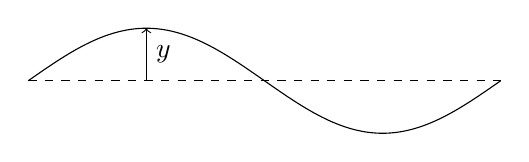
\begin{tikzpicture}
    \draw (0, 0) sin (1.5, 0.667) cos (3, 0) sin (4.5, -0.667) cos (6, 0);
    \draw [dashed] (0, 0) -- (6, 0);
    \draw [->] (1.5, 0) -- (1.5, 0.667) node [pos = 0.5, right] {$y$};
  \end{tikzpicture}
\end{center}
Suppose that $\rho(x)$ is the mass per unit length of a string. Then the restoring force on the string $\displaystyle ma = \rho \frac{\partial ^2 y}{\partial t^2}$ is proportional to the second derivative $\displaystyle\frac{\partial^2 y}{\partial x^2}$. So we obtain this wave equation.

\begin{remark}
  Why the second spatial derivative? The restoring force cannot depend on $y$ itself (translating the whole string causes no force) or on $\partial y/\partial x$ (a uniform slope has balanced forces). Only \emph{curvature}, measured by $\partial^2 y/\partial x^2$, produces a net restoring force.
\end{remark}

\subsubsection*{General solution (d'Alembert)}
Assuming $c$ is constant, we can factor the wave operator:
\begin{align*}
  \frac{\partial ^2 y}{\partial t^2} - c^2 \frac{\partial^2 y}{\partial x^2} &= 0\\
  \left(\frac{\partial}{\partial t} + c\frac{\partial}{\partial x}\right)\left(\frac{\partial}{\partial t} - c\frac{\partial}{\partial x}\right) y &= 0
\end{align*}
If $y = f(x + ct)$, then $(\partial_t - c\partial_x)y = 0$, so the product of operators gives zero. Similarly, $y = g(x - ct)$ satisfies $(\partial_t + c\partial_x)y = 0$. Since the equation is linear:

\begin{prop}[d'Alembert's solution]
  The general solution to the wave equation $y_{tt} = c^2 y_{xx}$ is
  \[
    y = f(x + ct) + g(x - ct),
  \]
  where $f$ and $g$ are arbitrary twice-differentiable functions. This represents a superposition of a wave travelling left (with speed $c$) and a wave travelling right (with speed $c$).
\end{prop}

To verify this is the most general solution, substitute $\xi = x + ct$ and $\eta = x - ct$. The chain rule gives $y_{tt} - c^2 y_{xx} = -4c^2 y_{\xi\eta}$. Thus the wave equation becomes $y_{\xi\eta} = 0$, which integrates to $y = f(\xi) + g(\eta)$.

\begin{remark}
  How many conditions do we need for a unique solution? In ODEs, we simply count the order of the equation. In PDEs, we must count over all variables. For the wave equation (second-order in both $x$ and $t$), we need 2 boundary conditions and 2 initial conditions.
\end{remark}

For example, we can have:
\begin{itemize}
  \item Initial conditions: at $t = 0$,
    \begin{gather*}
      y = \frac{1}{1 + x^2}\\
      \frac{\partial y}{\partial t} = 0
    \end{gather*}
  \item Boundary conditions: $y \to 0$ as $x \to \pm \infty$.
\end{itemize}
We know that the solution has the form
\[
  y = f(x + ct) + g(x - ct).
\]
The first initial condition give
\[
  f(x) + g(x) = \frac{1}{1 + x^2}\tag{1}
\]
The second initial condition gives
\[
  \frac{\partial y}{\partial t} = cf'(x) - cg'(x)\tag{2} = 0
\]
From (2), we know that $f' = g'$. So $f$ and $g$ differ by a constant. wlog, we can assume that they are indeed equal, since if we had, say, $f = g + 2$, then we can let $y = (f(x + ct) + 1) + (g(x - ct) + 1)$ instead, and the new $f$ and $g$ are equal.

From (1), we must have
\[
  f(x) = g(x) = \frac{1}{2(1 + x^2)}
\]
So, overall,
\[
  y = \frac{1}{2}\left[\frac{1}{1 + (x + ct)^2} + \frac{1}{1 + (x - ct)^2}\right]
\]
Where we substituted $x$ for $x +ct$ and $x - ct$ in $f$ and $g$ respectively.

\subsection{The diffusion equation}
The \emph{diffusion equation} (or \emph{heat equation}) models heat conduction in a solid:
\[
  \frac{\partial T}{\partial t} = \kappa \frac{\partial^2 T}{\partial x^2},
\]
where $T(x, t)$ is the temperature and $\kappa > 0$ is the \emph{thermal diffusivity}. This is classified as a \emph{parabolic PDE}.

\begin{remark}
  Unlike the wave equation (where acceleration $\propto$ curvature), here the rate of change $\partial T/\partial t$ is directly proportional to curvature $\partial^2 T/\partial x^2$. This makes the diffusion equation \emph{dissipative}: irregularities smooth out over time rather than propagating as waves.
\end{remark}

\begin{eg}[Semi-infinite heated bar]
  Consider a semi-infinite bar ($x \geq 0$) that is initially at temperature zero, then heated at the end $x = 0$ for $t > 0$:

  Suppose $T(x,0) = 0$, $T(0, t) = H(t) =
  \begin{cases}
    0 & t < 0\\
    1 & t > 0
  \end{cases}$, and $T(x, t)\to 0$ as $x\to \infty$. In words, the bar is initially cold, then suddenly heated at one end.

  We seek a \emph{similarity solution}---a solution where $T$ depends on $x$ and $t$ only through a particular combination. The natural length scale for diffusion over time $t$ is $\sqrt{\kappa t}$, suggesting we try $T(x, t) = \theta(\eta)$ where
  \[
    \eta = \frac{x}{2\sqrt{\kappa t}}
  \]
  is the \emph{similarity variable}.

  Applying the chain rule, we have
  \begin{align*}
    \frac{\partial T}{\partial x} &= \frac{\d \theta}{\d \eta} \frac{\partial \eta}{\partial x}\\
    &= \frac{1}{2\sqrt{\kappa t}} \theta'(\eta)\\
    \frac{\partial^2 T}{\partial x^2} &= \frac{1}{2\sqrt{\kappa t}} \frac{\d\theta'}{\d\eta}\frac{\partial \eta}{\partial x}\\
    &= \frac{1}{4\kappa t}\theta''(\eta)\\
    \frac{\partial T}{\partial t} &= \frac{\d \theta}{\d \eta}\frac{\partial \eta}{\partial t}\\
    &= -\frac{1}{2}\frac{x}{2\sqrt{\kappa}}\frac{1}{t^{3/2}} \theta'(\eta)\\
    &= -\frac{\eta}{2t}\theta'(\eta)
  \end{align*}
  Putting this into the diffusion equation yields
  \begin{align*}
    -\frac{\eta}{2t}\theta' &= \kappa \frac{1}{4\kappa t}\theta''\\
    \theta'' + 2\eta\theta' &= 0
  \end{align*}
  This is an ordinary differential equation for $\theta(\eta)$. This can be seen as a first-order equation for $\theta'$ with non-constant coefficients. Use the integrating factor $\mu = \exp(\int 2\eta \;\d \eta) = e^{\eta^2}$. So
  \begin{align*}
    (e^{\eta^2}\theta')' &= 0\\
    \theta' &= Ae^{-\eta^2}\\
    \theta &= A\int_0^\eta e^{-u^2}\;\d u + B\\
    &= \alpha\erf(\eta) + B
  \end{align*}
  where $\erf(\eta) = \frac{2}{\sqrt{\pi}} \int_0^\eta e^{-u^2}\;\d u$ from statistics, and $\erf(\eta)\to 1$ as $\eta\to \infty$.

  Now look at the boundary and initial conditions, (recall $\eta = x/(2\sqrt{\kappa t})$) and express them in terms of $\eta$. As $x \to 0$, we have $\eta \to 0$. So $\theta = 1$ at $\eta = 0$.

  Also, if $x\to \infty, t\to 0^+$, then $\eta \to \infty$. So $\theta \to 0$ as $\eta \to \infty$.

  From $\theta(0) = 1$, we get $B = 1$. From $\theta \to 0$ as $\eta \to \infty$, we need $\alpha = -1$. Thus $\theta = 1 - \erf(\eta) = \erfc(\eta)$, the \emph{complementary error function}. The solution is
  \[
    T = \erfc\left(\frac{x}{2\sqrt{\kappa t}}\right).
  \]
  At any fixed time $t$, the temperature profile looks like:
  \begin{center}
    \begin{tikzpicture}[xscale=3]
      \draw [->] (0, 0) -- (2.1, 0) node [right] {$x$};
      \draw [->] (0, 0) -- (0, 3) node [above] {$T$};

      %% approximation of error function
      \draw [mblue, semithick, domain=0:2] plot (\x, {2.5 * (1 + 0.278393 * \x + 0.230389*\x*\x + 0.000972*\x*\x*\x + 0.078108 * \x*\x*\x*\x)^(-4)});
    \end{tikzpicture}
  \end{center}
  The heat penetrates a distance of order $\sqrt{\kappa t}$, which grows with time. For a finite bar of length $L$, we can treat it as semi-infinite provided $\sqrt{\kappa t} \ll L$, i.e., $t \ll L^2/\kappa$.
\end{eg}
\end{document}
